\documentclass[supercite]{Experimental_Report}

\title{~~~~~~数据结构实验~~~~~~}
\author{杨明欣}
%\coauthor{张三、李四}
\school{计算机科学与技术学院}
\classnum{CS2106}
\stunum{U202115514}
%\costunum{U202115631、U202115631}
\instructor{周全} % 该系列实验报告模板有华科大计院教师陈加忠制作
\date{2022年6月12日}

\usepackage{algorithm, multirow}
\usepackage{algpseudocode}
\usepackage{amsmath}
\usepackage{amsthm}
\usepackage{framed}
\usepackage{mathtools}
\usepackage{subcaption}
\usepackage{xltxtra} %提供了针对XeTeX的改进并且加入了XeTeX的LOGO, 自动调用xunicode宏包(提供Unicode字符宏)
\usepackage{bm}
\usepackage{tikz}
\usepackage{tikzscale}
\usepackage{pgfplots}
\usepackage{listings}
\usepackage{xcolor}
\usepackage{pifont}
%\usepackage{enumerate}

\pgfplotsset{compat=1.16}

\newcommand{\cfig}[3]{
  \begin{figure}[htb]
    \centering
    \includegraphics[width=#2\textwidth]{images/#1.tikz}
    \caption{#3}
    \label{fig:#1}
  \end{figure}
}

\newcommand{\sfig}[3]{
  \begin{subfigure}[b]{#2\textwidth}
    \includegraphics[width=\textwidth]{images/#1.tikz}
    \caption{#3}
    \label{fig:#1}
  \end{subfigure}
}

\newcommand{\xfig}[3]{
  \begin{figure}[htb]
    \centering
    #3
    \caption{#2}
    \label{fig:#1}
  \end{figure}
}

\lstset{
basicstyle=\small,                 % 设置整体的字体大小
frame=lines,                               % 设置代码块边框
showstringspaces=false,                % 不显示字符串中的空格
numbers=left,                               % 在左侧显示行号
breaklines=true,                           %对过长的代码自动换行
% numberstyle=\scriptsize\color{gray},    % 设置行号格式
%numberstyle=\color{darkgray},               % 设置行号格式
backgroundcolor=\color{white},              % 设置背景颜色
keywordstyle=\color{blue},                  % 设置关键字颜色
commentstyle=\it\color[RGB]{0,100,0},       % 设置代码注释的格式
stringstyle=\sl\color{red},                 % 设置字符串格式
xleftmargin = 2em,
%xrigntmargin = 2em,
}

\newcommand{\whiteding}[1]{\ding{\numexpr171+#1\relax}}

\newcommand{\rfig}[1]{\autoref{fig:#1}}
\newcommand{\ralg}[1]{\autoref{alg:#1}}
\newcommand{\rthm}[1]{\autoref{thm:#1}}
\newcommand{\rlem}[1]{\autoref{lem:#1}}
\newcommand{\reqn}[1]{\autoref{eqn:#1}}
\newcommand{\rtbl}[1]{\autoref{tbl:#1}}

\algnewcommand\Null{\textsc{null }}
\algnewcommand\algorithmicinput{\textbf{Input:}}
\algnewcommand\Input{\item[\algorithmicinput]}
\algnewcommand\algorithmicoutput{\textbf{Output:}}
\algnewcommand\Output{\item[\algorithmicoutput]}
\algnewcommand\algorithmicbreak{\textbf{break}}
\algnewcommand\Break{\algorithmicbreak}
\algnewcommand\algorithmiccontinue{\textbf{continue}}
\algnewcommand\Continue{\algorithmiccontinue}
\algnewcommand{\LeftCom}[1]{\State $\triangleright$ #1}

\newtheorem{thm}{定理}[section]
\newtheorem{lem}{引理}[section]

\colorlet{shadecolor}{black!15}

\theoremstyle{definition}
\newtheorem{alg}{算法}[section]

\def\thmautorefname~#1\null{定理~#1~\null}
\def\lemautorefname~#1\null{引理~#1~\null}
\def\algautorefname~#1\null{算法~#1~\null}

\begin{document}

\maketitle

\clearpage

\pagenumbering{Roman}

\tableofcontents[level=2]

\clearpage

\pagenumbering{arabic}

\section{基于顺序存储结构的线性表实现}

\subsection{问题描述}

线性表是最常用而且最简单的一种数据结构。简言之,一个线性表是n个数据元素的有限序列。线性表的存储结构分为顺序存储和链式存储。线性表的数据集合为\{a1,a2,…,an\},假设每个元素的类型均为ElemType。其中,除第一个元素a1外,每一个元素有且只有一个直接前驱元素,除了最后一个元素an外,每一个元素有且只有一个直接后继元素。数据元素之间的关系是一对一的关系。

在较复杂的线性表中,一个数据元素可以由若干个数据项组成。在这种情况下,常把数据元素称为记录,含有大量记录的线性表又称为文件。

本实验要求构造一个具有菜单的功能演示系统。其中,在主程序中完成函数调用所需实参值的准备以及执行结果的显示,并给出正确的操作提示。程序实现线性表的初始化、销毁线性表、清空线性表、线性表判空、求线性表表长、获得元素等基本功能,以及最大连续子数组和、和为K的子数组、顺序表排序等附加功能。可以选择以文件的形式进行存储和加载,将生成的线性表存入到相应的文件中,也可以从文件中获取线性表进行操作。同时实现多线性表管理,完成多线性表的添加、删除、选择等操作。


 \begin{figure}[H]
 	\centering
 	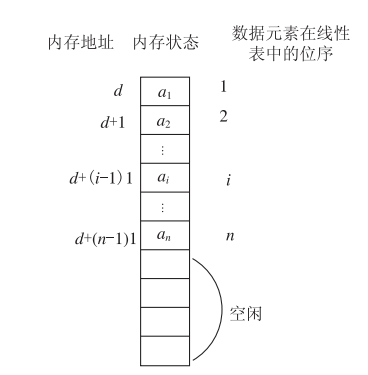
\includegraphics[width=0.6\textwidth]{images/线性表.png}
 	\caption{线性表存储结构}
 	\label{txlab}
 \end{figure}

\subsection{系统设计}

\subsubsection{头文件和预定义}

1、头文件

\begin{lstlisting}[language=c]
#include <stdio.h>
#include <stdlib.h>
#include <string.h>
#include <windows.h>
\end{lstlisting}

2、预定义常量

\begin{lstlisting}[language=c]
#define TRUE 1
#define FALSE 0
#define OK 1
#define ERROR 0
#define INFEASIBLE -1
#define OVERFLOW -2
#define LIST_INIT_SIZE 100
#define LISTINCREMENT  10.
#define MAXlength 10

\end{lstlisting}

3、类型表达式

\begin{lstlisting}[language=c]
typedef int status;
typedef int ElemType; //数据元素类型定义
typedef struct{  //顺序表(顺序结构)的定义
    ElemType * elem;
    int length;
    int listsize;
}SqList;
SqList L;

typedef struct{  //线性表的集合类型定义
    struct { char name[30];
        SqList L;
    } elem[11];
    int length;
}LISTS;
LISTS Lists;      //线性表集合的定义Lists

\end{lstlisting}

\subsubsection{基本功能函数}

 \begin{figure}[H]
 	\centering
 	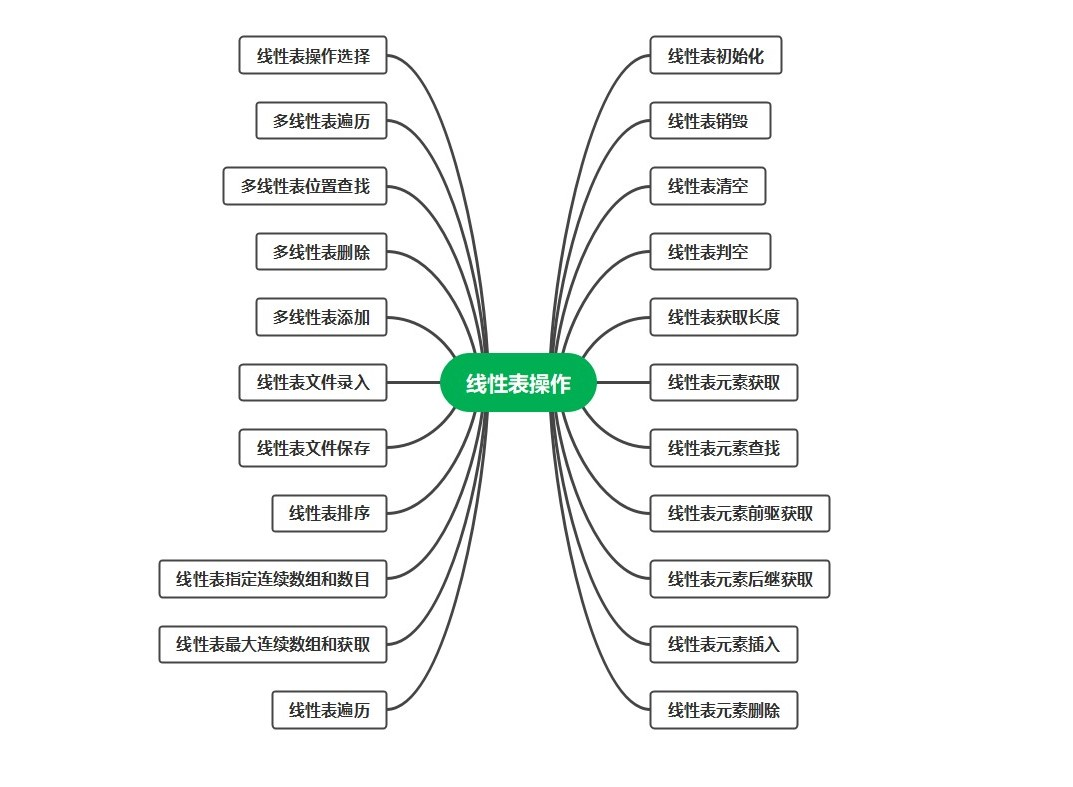
\includegraphics[width=0.9\textwidth]{images/线性表操作.jpg}
 	\caption{系统整体功能设计图}
 	\label{txlab}
 \end{figure}

线性表的逻辑结构定义如下:

ADT List\{

数据对象:D= $\{ a_{i} | a_{i} \in ElemSet,i=1,2,\cdots,n,n≥0\}$

数据关系:R1=$\{ <a_{i-1},a_{i}> | a_{i-1},a_{i}\in D,i=2,\cdots,n\}$

\}

依据最小完备性和常用性相结合的原则,以函数形式定义了线性表的初始化表、销毁表、清空表、判定空表、求表长和获得元素等12种基本运算,具体运算功能定义如下:

\begin{enumerate}
    \item 初始化表:函数名称是InitList(L);初始条件是线性表L不存在;操作结果是构造一个空的线性表;
    \item 销毁表:函数名称是DestroyList(L);初始条件是线性表L已存在;操作结果是销毁线性表L;
    \item 清空表:函数名称是ClearList(L);初始条件是线性表L已存在;操作结果是将L重置为空表;
    \item 判定空表:函数名称是ListEmpty(L);初始条件是线性表L已存在;操作结果是若L为空表则返回TRUE,否则返回FALSE;
    \item 求表长:函数名称是ListLength(L);初始条件是线性表已存在;操作结果是返回L中数据元素的个数;
    \item 获得元素:函数名称是GetElem(L,i,e);初始条件是线性表已存在,同时需要满足1≤i≤ListLength(L);操作结果是用e返回L中第i个数据元素的值;
    \item 查找元素:函数名称是LocateElem(L,e,compare());初始条件是线性表已存在;操作结果是返回L中第1个与e满足关系compare()关系的数据元素的位序,若这样的数据元素不存在,则返回值为0;
	\item 获得前驱:函数名称是PriorElem(L,cur\_e,pre\_e);初始条件是线性表L已存在;操作结果是若cur\_e是L的数据元素,且不是第一个,则用pre\_e返回它的前驱,否则操作失败,pre\_e无定义;
	\item 获得后继:函数名称是NextElem(L,cur\_e,next\_e);初始条件是线性表L已存在;操作结果是若cur\_e是L的数据元素,且不是最后一个,则用next\_e返回它的后继,否则操作失败,next\_e无定义;
	\item 插入元素:函数名称是ListInsert(L,i,e);初始条件是线性表L已存在,同时需要满足1≤i≤ListLength(L)+1;操作结果是在L的第i个位置之前插入新的数据元素e。
	\item 删除元素:函数名称是ListDelete(L,i,e);初始条件是线性表L已存在且非空,1≤i≤ListLength(L);操作结果:删除L的第i个数据元素,用e返回其值;
	\item 遍历表:函数名称是ListTraverse(L,visit()),初始条件是线性表L已存在;操作结果是依次对L的每个数据元素调用函数visit()。
\end{enumerate}

\subsubsection{附加功能函数}

\begin{enumerate}
    \item 最大连续子数组和:函数名称是MaxSubArray(L); 初始条件是线性表L已存在且非空,请找出一个具有最大和的连续子数组(子数组最少包含一个元素),操作结果是其最大和;
    \item 和为K的子数组:函数名称是SubArrayNum(L,k); 初始条件是线性表L已存在且非空, 操作结果是该数组中和为k的连续子数组的个数;
    \item 顺序表排序:函数名称是sortList(L);初始条件是线性表L已存在;操作结果是将L由小到大排序;
    \item 实现线性表的文件形式保存:其中,\whiteding{1}需要设计文件数据记录格式,以高效保存线性表数据逻辑结构(D,{R})的完整信息;\whiteding{2}需要设计线性表文件保存和加载操作合理模式。
	\begin{enumerate}
	\item 文件写入:函数名称是 SaveList(L,FileName);初始条件是线性表L已存在;操作结果是将L的元素写到名称为FileName的文件中。
	\item 文件读出:函数名称是 LoadList(L,FileName);初始条件是线性表 L 不存在;操作结果是将文件 FileName 中的元素读到表 L中。
	\end{enumerate}
    \item 实现多个线性表管理:设计相应的数据结构管理多个线性表的查找、添加、移除等功能。
	\begin{enumerate}
	\item 增加线性表:函数名称是 AddList(Lists, ListName);初始条件是名称为ListName的线性表不存在于线性表集合中;操作结果是在 Lists中创建一个名称为ListName 的初始化好的线性表。
	\item 移除线性表:函数名称是RemoveList(Lists, ListName);初始条件是名称为ListName的线性表存在于线性表集合中;操作结果是将该线性表移除。
	\item 查找线性表:函数名称是LocateList(Lists, ListName);初始条件是名称为ListName的线性表存在于线性表集合中;操作结果是返回该线性表在Lists中的逻辑索引。
	\item 遍历所有表:函数名称是TraverseList(Lists,visit());初始条件是Lists已存在;操作结果是对所有的表遍历并输出。
	\item 选择表:函数名称是 SelectList (Lists, i);初始条件是Lists已存在,1≤i≤Lists.Length+1;操作结果是将Lists中逻辑索引为i的线性表选择为当前处理的线性表,以便后续再调用其他函数对该表进行操作。
	\end{enumerate}
\end{enumerate}

\subsubsection{演示系统}

构造一个具有菜单的功能演示系统。其中,在主程序中完成函数调用所需实参值的准备和函数执行结果的显示,并给出适当的操作提示显示。

该演示系统具有完备性,包含每一功能的中英文说明和注意事项,同时显示当前线性表名称和初始化情况。

输入1$\sim$ 22可以调用上述的22个函数,对线性表或多线性表进行操作;输入0时退出系统。



\subsection{系统实现}

\subsubsection{演示系统框架}

系统主体通过while循环实现多次选择,通过op获取用户的选择,通过switch语句根据用户选择实现具体功能,通过system("cls")语句实现清屏操作,保证界面整洁和满足用户体验感。

具体实现为将菜单和功能实现写入到 while 循环中,用op 获取用户的选择,op初始化为 1,以便第一次能进入循环。进入循环后,用户输入选择 0$\sim$22,其中 1$\sim$22 分别代表线性表的一个基本运算,在主函数中通过 switch语句对应到相应的函数功能,执行完该功能后通过 break 跳出switch 语句,继续执行 while 循环,直至用户输入 0 退出当前演示系统。系统初进入时默认对默认线性表(未创建)进行操作,后续可增加新表并进行选择,实现多线性表操作。

\subsubsection{数据结构设计}

\begin{enumerate}
	\item 线性表:线性表中用数组elem储存数据,定义length变量储存线性表长度,定义listsize变量表示线性表的大小。
	\item 多线性表的管理表:定义length变量表示管理表的长度。定义elem数组顺序储存线性表及其名称。
	\end{enumerate}

\subsubsection{函数思想及实现}

\textbf{说明:无特殊说明情况下,每一函数均需判断线性表是否存在之后,再对线性表进行相应的操作。}

线性表基本功能函数的实现:

\paragraph{ 1.} status InitList (SqList \&L)

输入:线性表(引用参数)

输出:函数运行状态

函数思想描述:将线性表初始化过程写成函数,其中传入函数的参数是全局定义的结构体类型变量L 的引用,在函数中,首先使用 malloc 函数为线性表分配LISTSIZE 大小的连续内存空间,将首地址赋值给 L.elem,由于线性表的长度为 0,将 L.length 初始化为 0,即完成了线性表的初始化。

\paragraph{ 2.} status DestroyList (SqList \&L)

输入:线性表(引用参数)

输出:函数运行状态

函数思想描述:将销毁线性表的过程写成函数,其中将定义的结构体类型变量L的引用作为函数参数。在函数中,首先使用 free 函数释放掉以 L.elem为首地址的连续内存空间,再将L.length重新赋值为0,完成线性表的销毁。


\paragraph{ 3.}status ClearList (SqList \&L)

输入:线性表(引用参数)

输出:函数运行状态

函数思想描述:将清空线性表的过程写成函数,其中将定义的结构体类型变量L的引用作为函数参数。在函数中,无需对于L.elem内的元素进行处理,直接将L.length 赋值为0即可,即完成了线性表的清空。


\paragraph{ 4.}status ListEmpty (SqList L)

输入:线性表(传值调用)

输出:函数运行状态

函数思想描述:将求判断线性表是否为空写成函数,其中将定义的结构体类型变量L的值作为函数的参数,在函数中,如果线性表不存在,返回INFEASIBLE。如果线性表存在,则判断如果L.length为0,返回FALSE,否则返回TRUE。

\paragraph{ 5.}int ListLength (SqList L)

输入:线性表(传值调用)

输出:整型变量(含义为表 L 中元素数目)

函数思想描述:将求表长过程写成函数,其中将定义的结构体类型变量L的引用作为函数的参数,在函数中,直接返回 L.length
即为所求线性表的表长。

\paragraph{ 6.}status GetElem (SqList L, int i, ElemType \&e)

输入:线性表(传值调用),整型变量(元素逻辑索引),类型变量(引用参数,用于存储元素)

输出:函数运行状态

函数思想描述:将获得线性表元素写成函数,其中函数的参数是结构体类型变量L 以及数据元素的逻辑索引i,首先需要判断输入的元素序号i的合法性(1≤i≤L.Length)。因为采取的是线性存储结构,所以直接通过访问数组元素的方式即 L.elem[i-1] 来获取元素存储到元素e中。

\paragraph{ 7.}status LocateElem (SqList L, ElemType e, int (*compare)(SqList, int, ElemType))

输入:线性表(传值调用),类型变量(含义为待查找的元素), 函数指针

输出:函数运行状态

函数思想描述:将查找线性表特定元素写成函数,其中函数的参数是定义的结构体类型变量L以及待查找的数据元素值,通过遍历线性表中的每一个元素查找值为e的元素,即compare(L,i,e)为1,返回该元素的逻辑索引(即位序),如果元素不存在,则返回0。

\paragraph{ 8.}status PriorElem (SqList L, ElemType e, ElemType \&pre)

输入:线性表(传值调用),类型变量(传值调用),类型变量(引用参数,用于存储元素)

输出:函数运行状态

函数思想描述:将获得前驱过程写成函数,函数的参数是结构体类型变量L以及特定数据元素的值,存储前驱元素的变量作为另一个参数。首先调用LocateElem(L, e)函数判断该线性表中特定数据元素的位序并转换为数组下标i,判断数组下标是否合法(1≤i≤L.Length-1),则将元素的前驱赋值给pre变量,返回OK;否则返回ERROR。

\paragraph{ 9.}status NextElem (SqList L, ElemType e, ElemType \&next)

输入:线性表(传值调用),类型变量(传值调用),类型变量(引用参数,用于存储元素)

输出:函数运行状态

函数思想描述:将获得后继过程写成函数,函数的参数是结构体类型变量L以及特定数据元素的值,存储后继元素的变量作为另一个参数。首先调用LocateElem(L, e)函数判断该线性表中特定数据元素的位序并转换为数组下标i,判断数组下标是否合法(0≤i≤L.Length-2),则将元素的后继赋值给pre变量,返回OK;否则返回ERROR。

\paragraph{10.}status ListInsert (SqList L, int i, ElemType e)

输入:线性表(传值调用),整型变量(元素位序),类型变量(含义为待插入的元素值)

输出:函数运行状态

函数思想描述:将插入元素的过程写成函数,函数的参数是结构体类型变量L,插入元素的位序i和待插入的元素的值e。在函数中,首先判断插入位置的合法性(1≤i≤L.Length+1)。其次判断当前线性表存储空间是否已满,即判断L.length和L.listsize,如果线性表已满,则使用 realloc 函数为线性表重新分配空间。插入元素时,先将位序为i后的元素向后移动一个内存单元,然后将e插入进去,返回OK。

\paragraph{11.}status ListDelete (SqList L, int i , ElemType \&e)

输入:线性表(传值调用),整型变量(元素位序),类型变量(引用参数,用于存储被删除元素)

输出:函数运行状态

函数思想描述:将删除线性表中元素写成函数,函数的参数是结构体类型变量L,删除元素的位序i和存储被删除元素的变量。首先判断位序的合法性(1≤i≤L.Length),将被删除的元素赋值给e,然后将位序为i后的元素向后移动一个内存单元,返回OK。

\paragraph{12.}status ListTraverse (SqList L,int (*visit)(SqList,int))

输入:线性表

输出:函数运行状态

函数思想描述:将遍历线性表写成一个函数,函数的参数是结构体类型变量L,遍历数组中的每一个元素并调用visit()函数,如果线性表为空,则输出线性表为空。


附加功能函数的实现:

\paragraph{13.}status MaxSubArray(SqList L)

输入:线性表(传值调用)

输出:整型变量(含义为连续数组和的最大值)

算法描述:函数通过将线性表队列化,用max记录前缀和,通过每次判断前缀是否为负,若为负,则从头开始依次出队列直至前缀为正,保证遍历每一组和为正的连续数组,通过temp记录连续数组和的最大值,最后返回temp。

时间复杂度:O($n^{2}$)

空间复杂度:O(1)

\paragraph{14.}status SubArrayNum(SqList L, int k)

输入:线性表(传值调用)、整型变量(含义为连续数组和)

输出:整型变量(线性表中连续数组和为k的连续数组数目 )

函数思想描述:通过牺牲空间换取时间的算法思想,额外增添一前缀和数组,通过前缀和数组间的差值可以计算连续数组和,使用count计数连续数组和为k的数组数目。此算法可以将时间复杂度降到O($n^{2}$),具体算法流程图如下:

 \begin{figure}[H]
 	\centering
 	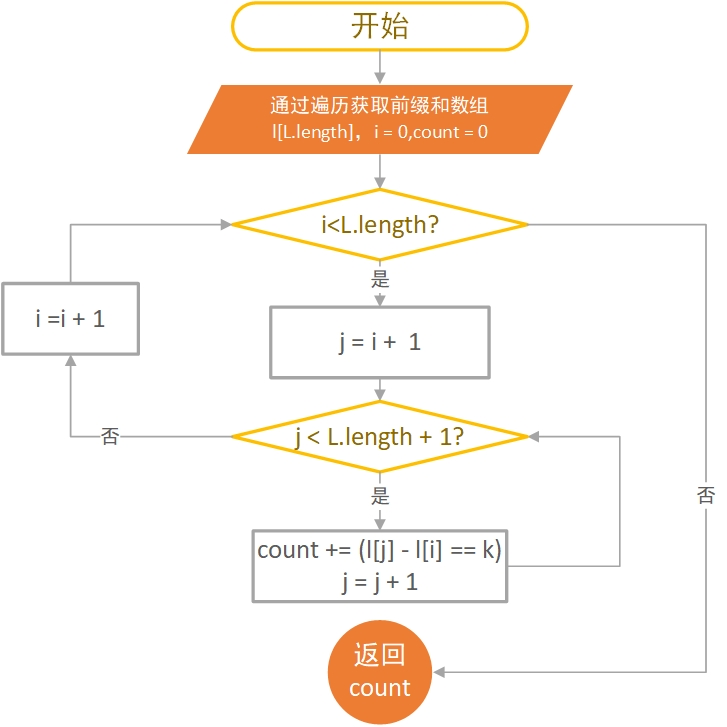
\includegraphics[width=0.6\textwidth]{images/连续数组.jpg}
 	\caption{连续数组和数目程序流程图}
 	\label{txlab}
 \end{figure}

时间复杂度:O($n^{2}$)

空间复杂度:O(n)

\paragraph{15.}status sortList(SqList\& L)

输入:线性表(引用参数)

输出:整型变量(线性表中连续数组和为k的连续数组数目)

函数思想描述:函数实现线性表排序。该函数通过归并排序算法将线性表进行排序。

 \begin{figure}[H]
 	\centering
 	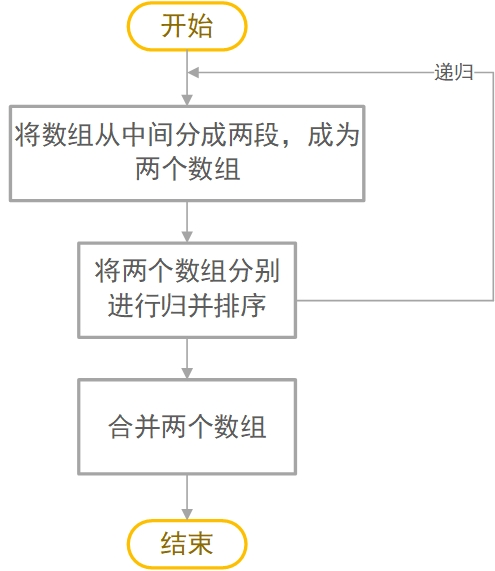
\includegraphics[width=0.5\textwidth]{images/归并排序.jpg}
 	\caption{归并排序文字流程图}
 	\label{txlab}
 \end{figure}


时间复杂度:O($nlogn$)

空间复杂度:O(n)

\paragraph{16.}status SaveList (SqList L, char FileName [])

输入:线性表(传值调用),字符串变量(含义为文件名称)

输出:函数运行状态

函数思想描述:将保存线性表为文件写成函数,函数的参数是结构体类型变量L和文件名称FileName。首先判断线性表是否存在,如果存在,然后判断文件内是否有内容,文件为空或不存在时则打开或创建文件,然后调用fwrite函数将表中的所有元素写入该文件中,之后关闭文件。

\paragraph{17.}status LoadList (SqList L, char FileName [])

输入:线性表(传值调用),字符串变量(含义为文件名称)

输出:函数运行状态

函数思想描述:将读取文件中的线性表写成函数,函数的参数是结构体类型变量L和文件名称FileName。首先判断 L 是否存在,如果线性表 L 存在,表示 L 中已经有数据,读入数据会覆盖原数据造成数据丢失,故只有 L 不存在时才可以继续操作。然后打开文件,调用fread函数将所有元素写入表中,之后关闭文件。

\paragraph{18.}status AddList (LISTS Lists, char ListName [])

输入:顺序表数组,字符串变量(含义为线性表名称)

输出:函数运行状态

函数思想描述:将增加线性表写成函数,函数的参数是 LISTS 结构体类型变量和线性表名称ListName。Lists 是一个以顺序表形式管理的线性表的集合,在集合中增加一个新的空线性表,并将表名称存储在该表的 name 分量当中。在添加线性表之前,应当判断表名是否唯一。

\paragraph{19.}status RemoveList (LISTS List, char ListName [])

输入:顺序表数组,字符串变量(含义为线性表名称)

输出:函数运行状态

函数思想描述:将移除线性表写成函数,函数的参数是 LISTS 结构体类型变量和线性表名称ListName。在 Lists 中查找名称为 ListName 的线性表,如果可以找到,则调用DestroyList函数将其删除。

\paragraph{20.}int LocateList (LISTS Lists, char ListName [])

输入:顺序表数组,字符串变量(含义为线性表名称)

输出:整型变量(线性表的位序)

函数思想描述:将查找线性表写成函数,函数的参数是 LISTS 结构类型变量和线性表名称ListName。在 Lists 中查找名称为 ListName 的线性表,如果可以找到,返回线性表的逻辑索引,否则返回 0。

\paragraph{21.}status TraverseList(LISTS Lists)

输入:顺序表数组

输出:函数运行状态

函数思想描述:函数的参数是 LISTS 结构类型变量。调用TraverseList函数遍历线性表集合中每一个线性表,输出每一个线性表的名称。

时间复杂度:O(mn)

\paragraph{22.}status SelectList(LISTS Lists, int i)

输入:顺序表数组,整型变量(含义为线性表的逻辑索引)

输出:函数运行状态

函数思想描述:将选择线性表写成函数,函数的参数是 LISTS 结构类型变量和逻辑索引。将 Lists 中逻辑索引为i的线性表赋值给L,后续可调用其它函数时将对此表进行操作。

\subsection{系统测试}

系统菜单整体布局如图:

 \begin{figure}[H]
 	\centering
 	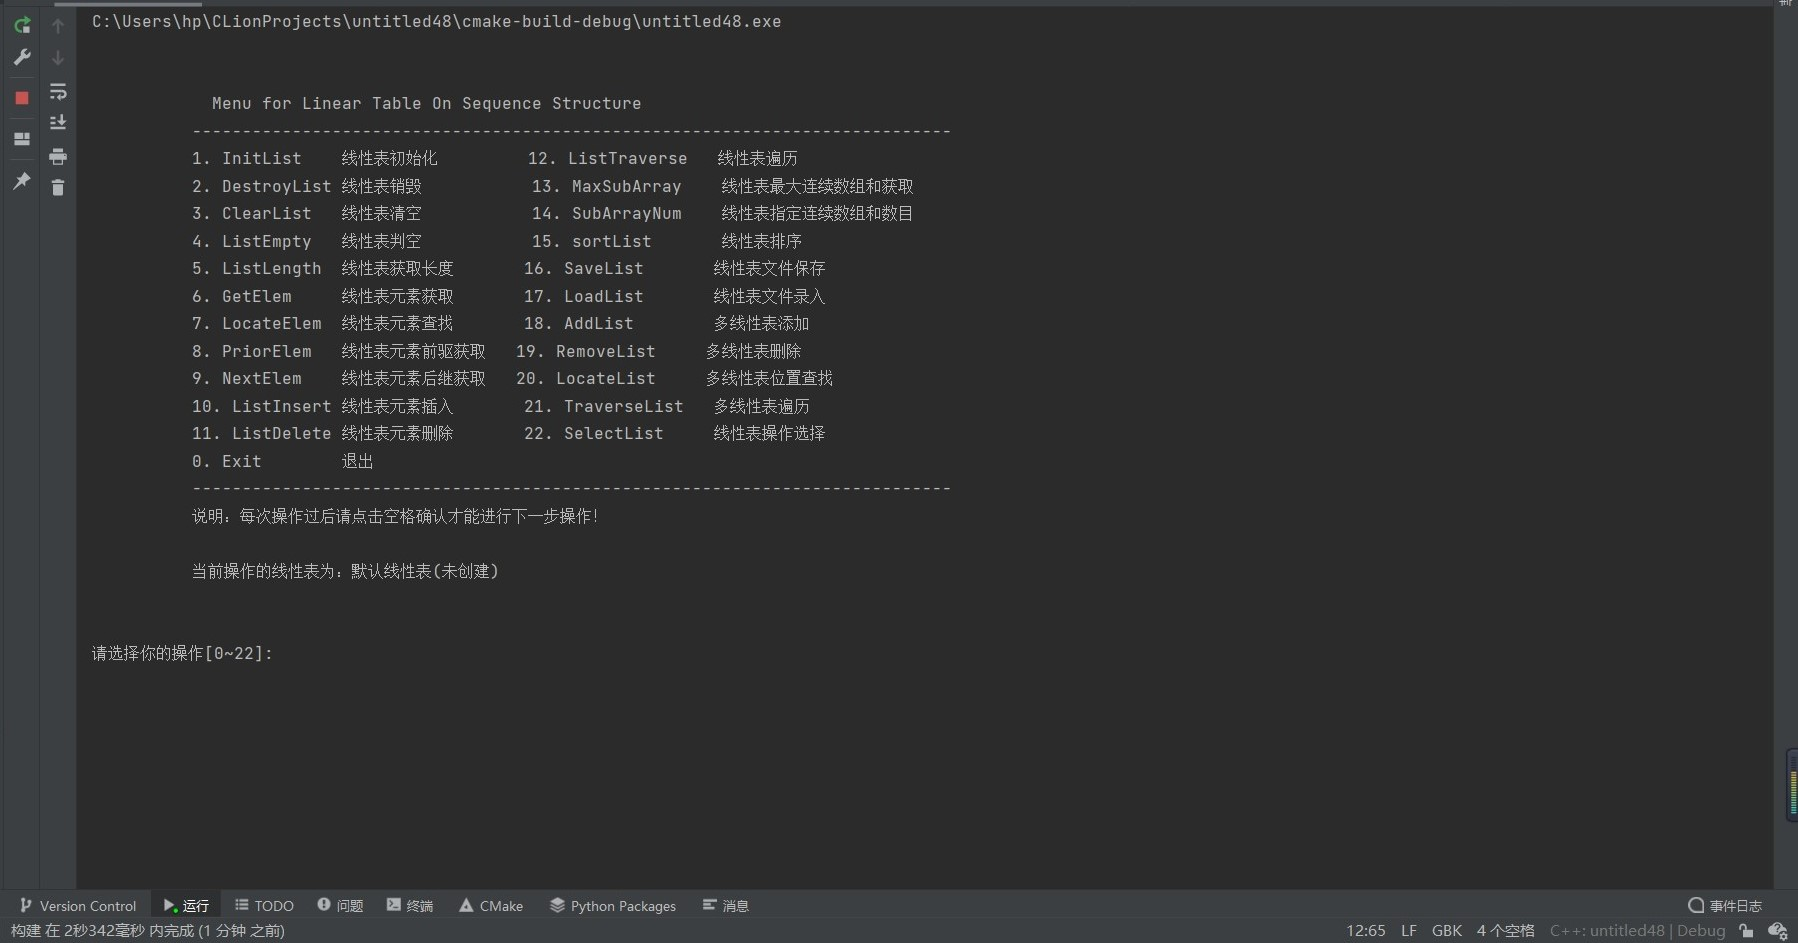
\includegraphics[width=0.8\textwidth]{images/菜单.jpg}
 	\caption{菜单}
 	\label{txlab}
 \end{figure}

测试集如下:

测试集1:线性表中存有元素1 3 5 7 9

测试集2:线性表中存有元素1 2 3 4 5 6 7 8 9 10 11 12 13 14 15 16 17 18 19 20

测试集3:线性表集合中有两个线性表 FirstList: 1 3 5 7 9;SecondList: 2 4 6 8 10

测试集4:线性表中存有元素 -2 1 -3 4 -1 2 1 -5 4

\setcounter{paragraph}{0}

\subsubsection{基本功能函数测试}

\paragraph{ 1.}InitList测试

测试1:测试函数是否能成功创建线性表;

测试2:测试当线性表已经存在时,函数是否能再次创建线性表。

\vspace{0.5em}

\begin{tabular}{|c|l|c|c|c|}
	\hline
	测试编号 & 测试输入 & 预期结果 & 实际运行结果 \\
	\hline
	1 & 1 & 线性表创建成功 & 一致 \\
	\hline
	2 & 1$\rightarrow$1 & 线性表创建失败 & 一致 \\
	\hline
\end{tabular}

~\

 \begin{figure}[H]
 	\centering
 	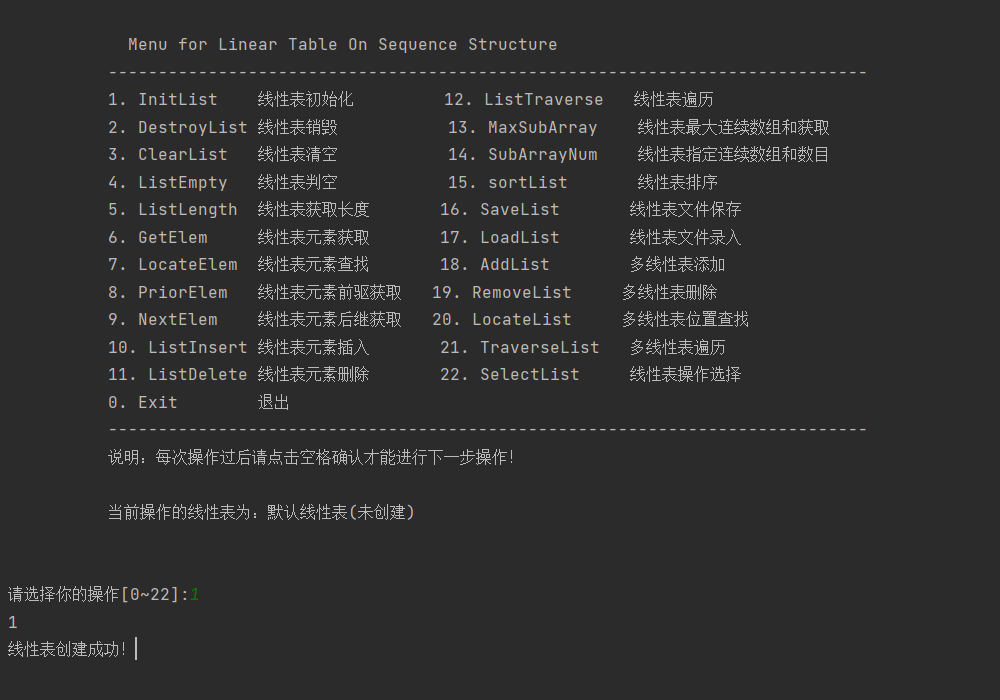
\includegraphics[width=0.6\textwidth]{images/线性表测试1.png}
 	\caption{测试1运行结果}
 	\label{txlab}
 \end{figure}


\paragraph{ 2.}DestroyList测试

测试1:测试函数是否能对不存在的线性表进行销毁;

测试2:测试函数是否能对已经存在的线性表进行销毁;

测试3:将测试在销毁线性表之后检测能否重新创建线性表。

\vspace{0.5em}

\begin{tabular}{|c|l|c|c|c|}
	\hline
	测试编号 & 测试输入 & 预期结果 & 实际运行结果 \\
	\hline
	1 & 2 & 线性表不存在,销毁失败 & 一致 \\
	\hline
	2 & 1$\rightarrow$2 & 线性表销毁成功 & 一致 \\
	\hline
	3 & 1$\rightarrow$2$\rightarrow$1 & 线性表销毁成功;线性表创建成功 & 一致 \\
	\hline
\end{tabular}

~\

 \begin{figure}[H]
 	\centering
 	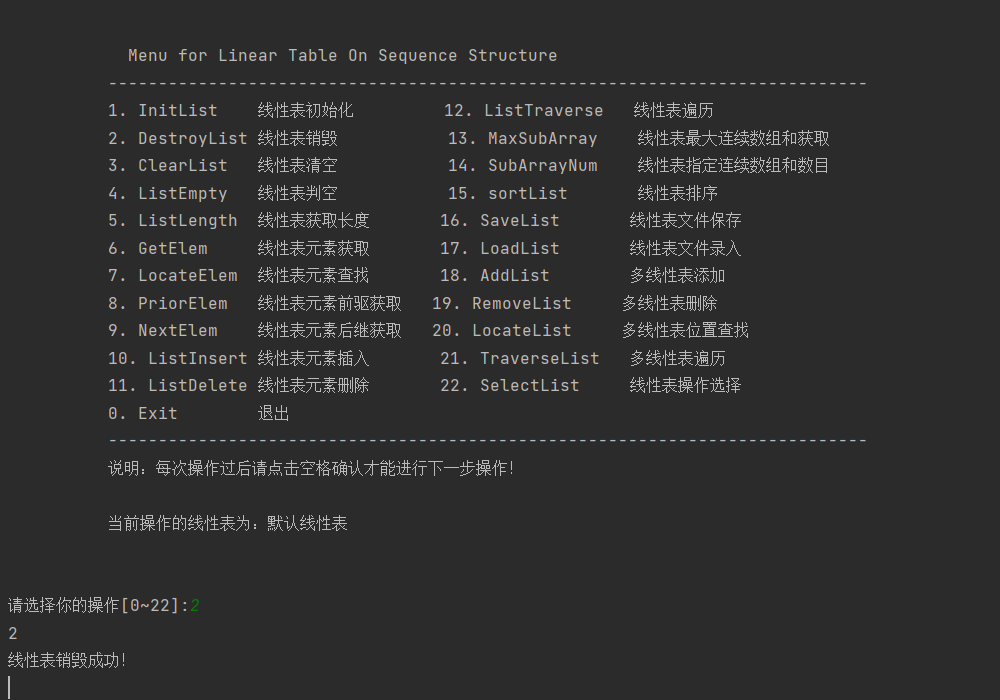
\includegraphics[width=0.6\textwidth]{images/线性表测试2.png}
 	\caption{测试2运行结果}
 	\label{txlab}
 \end{figure}


\paragraph{ 3.}ClearList测试

测试1:测试函数是否能对不存在的线性表进行清空;

测试2:测试函数是否能对已经存在的线性表进行清空;

测试3:在测试集1的情况下进行,在调用ClearList之后,通过求线性表的表长,来判断线性表中的元素是否确实被清空。

\vspace{0.5em}

\begin{tabular}{|c|l|c|c|c|}
	\hline
	测试编号 & 测试输入 & 预期结果 & 实际运行结果 \\
	\hline
	1 & 3 & 线性表不存在,清空失败 & 一致 \\
	\hline
	2 & 1$\rightarrow$3 & 线性表清空成功 & 一致 \\
	\hline
	3 & 1$\rightarrow$测试集1$\rightarrow$3$\rightarrow$5 & 线性表长度为0 & 一致 \\
	\hline
\end{tabular}

~\

 \begin{figure}[H]
 	\centering
 	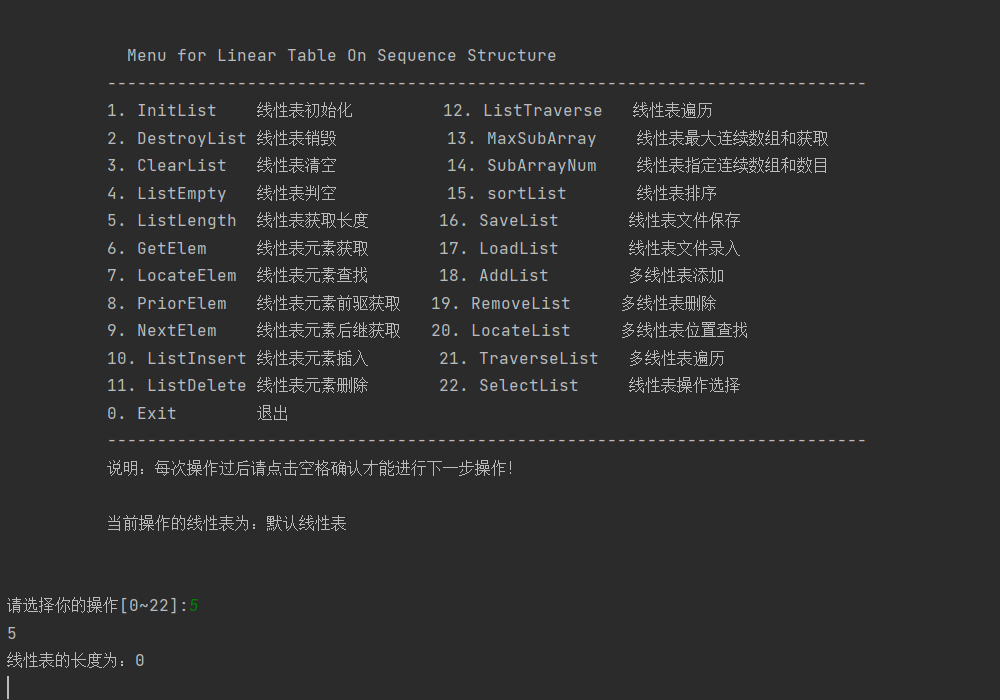
\includegraphics[width=0.6\textwidth]{images/线性表测试3.png}
 	\caption{测试3运行结果}
 	\label{txlab}
 \end{figure}


\paragraph{ 4.}ListEmpty测试

测试1:测试函数能否对不存在的线性表判空;

测试2:测试函数能否正确判断空线性表;

测试3:在测试集1的情况下进行,测试函数能否正确判断空线性表。

\vspace{0.5em}

\begin{tabular}{|c|l|c|c|c|}
	\hline
	测试编号 & 测试输入 & 预期结果 & 实际运行结果 \\
	\hline
	1 & 4 & 线性表不存在,判空失败 & 一致 \\
	\hline
	2 & 1$\rightarrow$4 & 线性表为空 & 一致 \\
	\hline
	3 & 1$\rightarrow$测试集1$\rightarrow$4 & 线性表非空 & 一致 \\
	\hline
\end{tabular}

~\

 \begin{figure}[H]
 	\centering
 	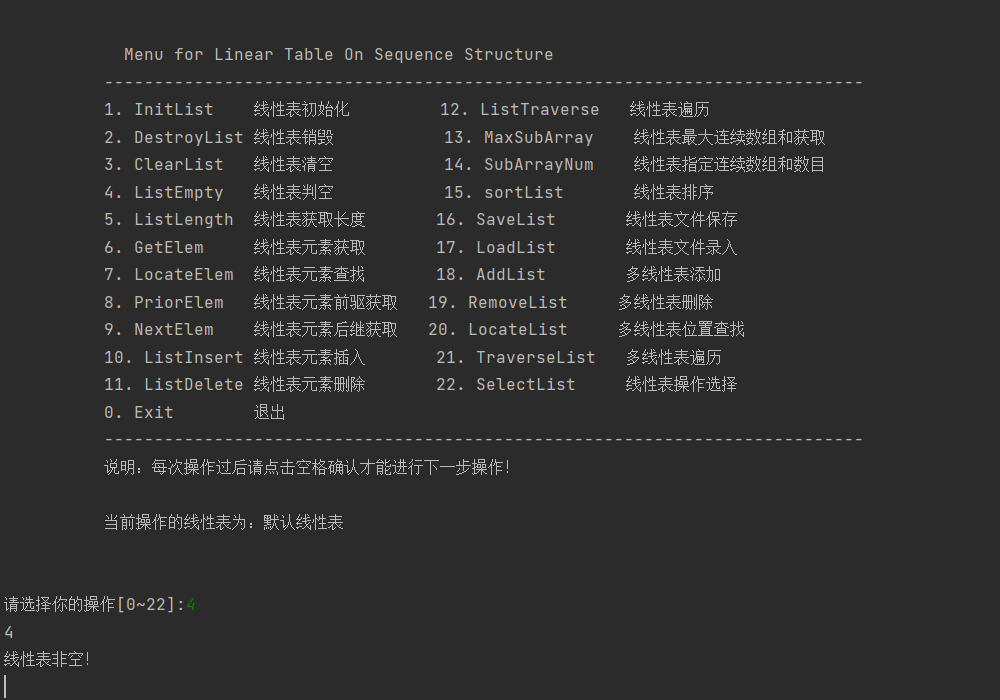
\includegraphics[width=0.6\textwidth]{images/线性表测试4.png}
 	\caption{测试3运行结果}
 	\label{txlab}
 \end{figure}


\paragraph{ 5.}ListLength测试


测试1:测试函数能否对不存在的线性表求长;

测试2:测试函数能否正确求出空线性表的长度;

测试3:在测试集1的情况下进行,测试函数能否正确求出线性表的长度。

\vspace{0.5em}

\begin{tabular}{|c|l|c|c|c|}
	\hline
	测试编号 & 测试输入 & 预期结果 & 实际运行结果 \\
	\hline
	1 & 5 & 线性表不存在,求长失败 & 一致 \\
	\hline
	2 & 1$\rightarrow$5 & 线性表长度为0 & 一致 \\
	\hline
	3 & 1$\rightarrow$测试集1$\rightarrow$5 & 线性表长度为5 & 一致 \\
	\hline
\end{tabular}

~\

 \begin{figure}[H]
 	\centering
 	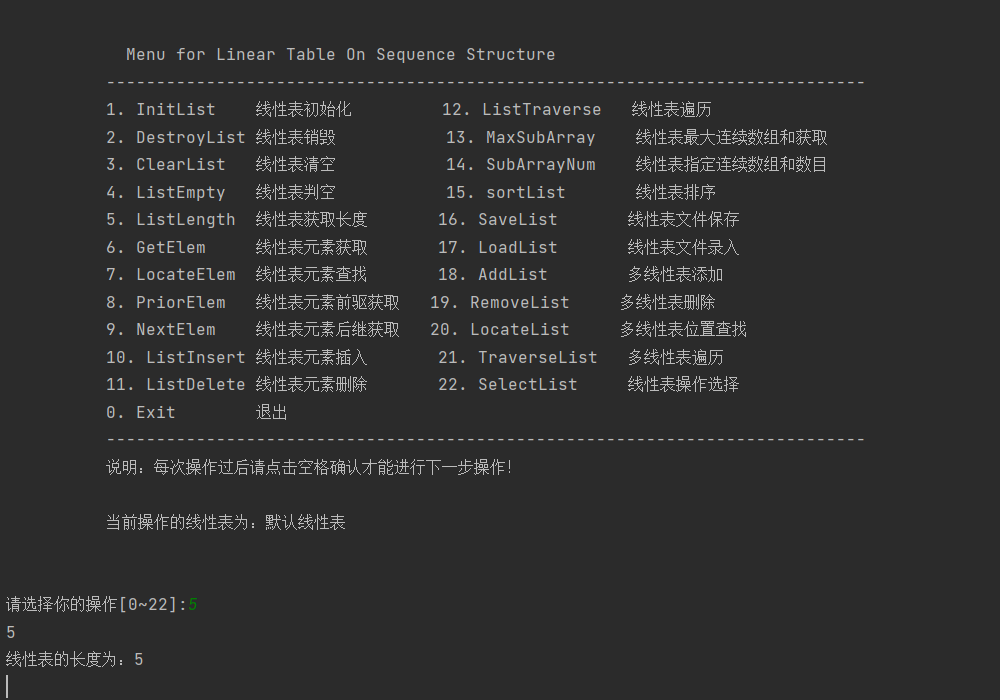
\includegraphics[width=0.6\textwidth]{images/线性表测试5.png}
 	\caption{测试1运行结果}
 	\label{txlab}
 \end{figure}


\paragraph{ 6.}GetElem测试

此函数的所有测试将在测试集1的情况下进行。

测试1,2:将测试函数能否正确找到元素;

测试3,4,5:将测试函数能否正确识别非法的位序。

\vspace{0.5em}

\begin{tabular}{|c|l|c|c|}
	\hline
	测试编号 & 测试输入 & 预期结果 & 实际运行结果 \\
	\hline
	1 & 6$\rightarrow$2 & 线性表中第2个元素为3 & 一致 \\
	\hline
	2 & 6$\rightarrow$5 & 线性表中第5个元素为9 & 一致 \\
	\hline
	3 & 6$\rightarrow$-1 & 输入的逻辑索引不合法! & 一致 \\
	\hline
	4 & 6$\rightarrow$0 & 输入的逻辑索引不合法! & 一致 \\
	\hline
	5 & 6$\rightarrow$6 & 输入的逻辑索引不合法! & 一致 \\
	\hline
\end{tabular}


~\

 \begin{figure}[H]
 	\centering
 	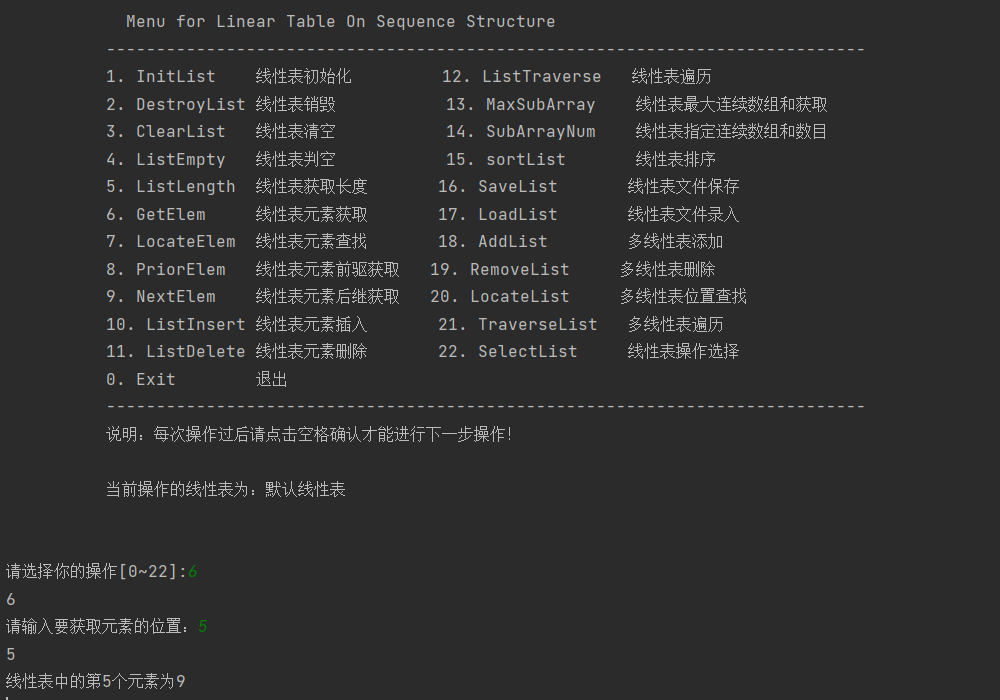
\includegraphics[width=0.6\textwidth]{images/线性表测试6.png}
 	\caption{测试2运行结果}
 	\label{txlab}
 \end{figure}



\paragraph{ 7.}LocateElem测试

此函数的所有测试将在测试集1的情况下进行。

测试1,2:将测试函数能否正确找到位序;

测试3,4:将测试函数能否正确识别不在线性表中的元素。

\vspace{0.5em}

\begin{tabular}{|c|l|c|c|}
	\hline
	测试编号 & 测试输入 & 预期结果 & 实际运行结果 \\
	\hline
	1 & 7$\rightarrow$1 & 该元素存在且元素逻辑索引为:1 & 一致 \\
	\hline
	2 & 7$\rightarrow$9 & 该元素存在且元素逻辑索引为:5 & 一致 \\
	\hline
	3 & 7$\rightarrow$6 & 输入的元素不存在! & 一致 \\
	\hline
	4 & 7$\rightarrow$-1 & 输入的元素不存在! & 一致 \\
	\hline
\end{tabular}

~\

 \begin{figure}[H]
 	\centering
 	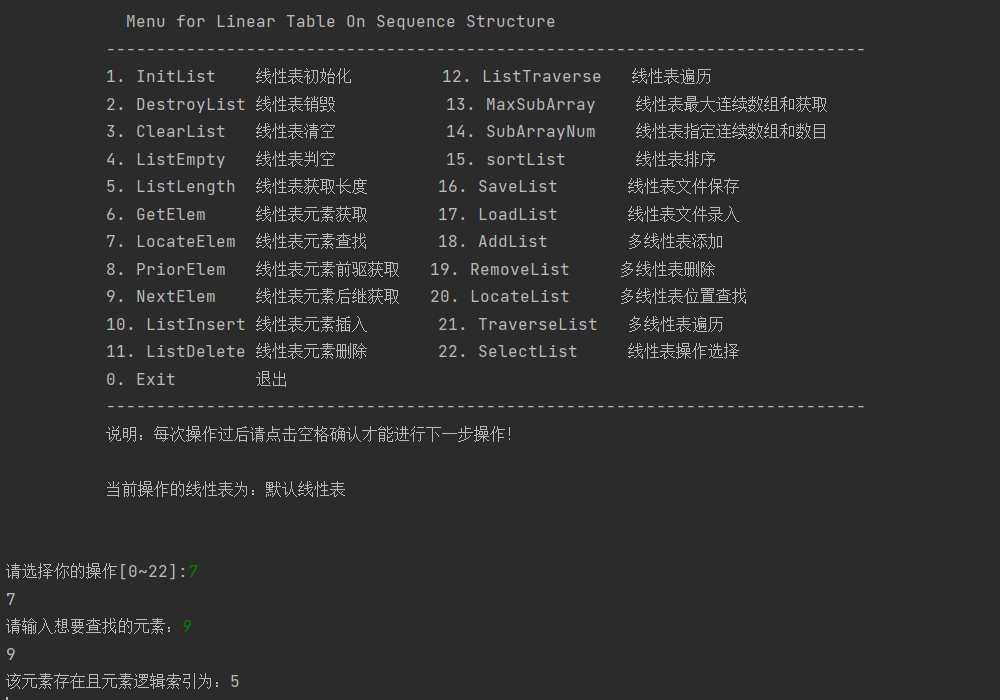
\includegraphics[width=0.6\textwidth]{images/线性表测试7.png}
 	\caption{测试2运行结果}
 	\label{txlab}
 \end{figure}


\paragraph{ 8.}PriorElem测试

    此函数的所有测试将在测试集1的情况下进行。

    测试1,2:将测试函数能否正确找到前驱;

    测试3:将测试函数能否正确判断第一个元素没有前驱;

    测试4:将测试函数能否正确判断不在线性表中的元素没有前驱。

\vspace{0.5em}

\begin{tabular}{|c|l|c|c|}
	\hline
	测试编号 & 测试输入 & 预期结果 & 实际运行结果 \\
	\hline
	1 & 8$\rightarrow$3 & 该元素存在且前驱元素为:1 & 一致 \\
	\hline
	2 & 8$\rightarrow$9 & 该元素存在且前驱元素为:7 & 一致 \\
	\hline
	3 & 8$\rightarrow$1 & 线性表中该元素不存在前驱! & 一致 \\
	\hline
	4 & 8$\rightarrow$6 & 线性表中该元素不存在! & 一致 \\
	\hline
\end{tabular}

~\

 \begin{figure}[H]
 	\centering
 	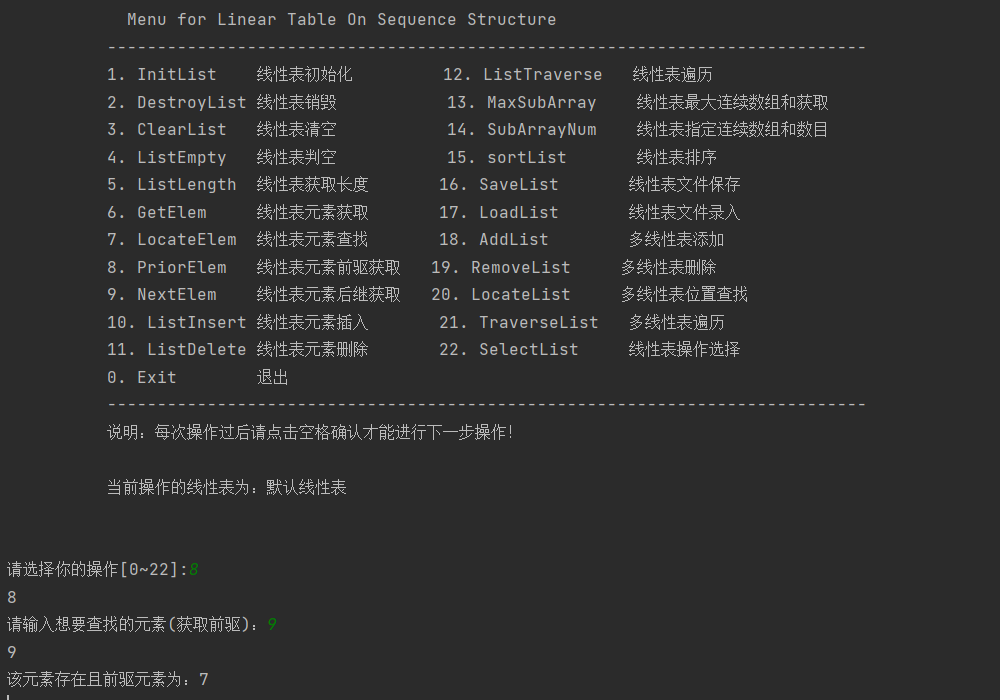
\includegraphics[width=0.6\textwidth]{images/线性表测试8.png}
 	\caption{测试2运行结果}
 	\label{txlab}
 \end{figure}


\paragraph{ 9.}NextElem测试

    此函数的所有测试将在测试集1的情况下进行。

    测试1,2:将测试函数能否正确找到后继;

    测试3:将测试函数能否正确判断最后一个元素没有后继;

    测试4:将测试函数能否正确判断不在线性表中的元素没有后继。

\vspace{0.5em}

\begin{tabular}{|c|l|c|c|}
	\hline
	测试编号 & 测试输入 & 预期结果 & 实际运行结果 \\
	\hline
	1 & 9$\rightarrow$3 & 线性表中该元素的后继为5 & 一致 \\
	\hline
	2 & 9$\rightarrow$7 & 线性表中该元素的后继为9 & 一致 \\
	\hline
	3 & 9$\rightarrow$9 & 线性表中该元素不存在后继! & 一致 \\
	\hline
	4 & 9$\rightarrow$6 & 线性表中该元素不存在! & 一致 \\
	\hline
\end{tabular}

~\

 \begin{figure}[H]
 	\centering
 	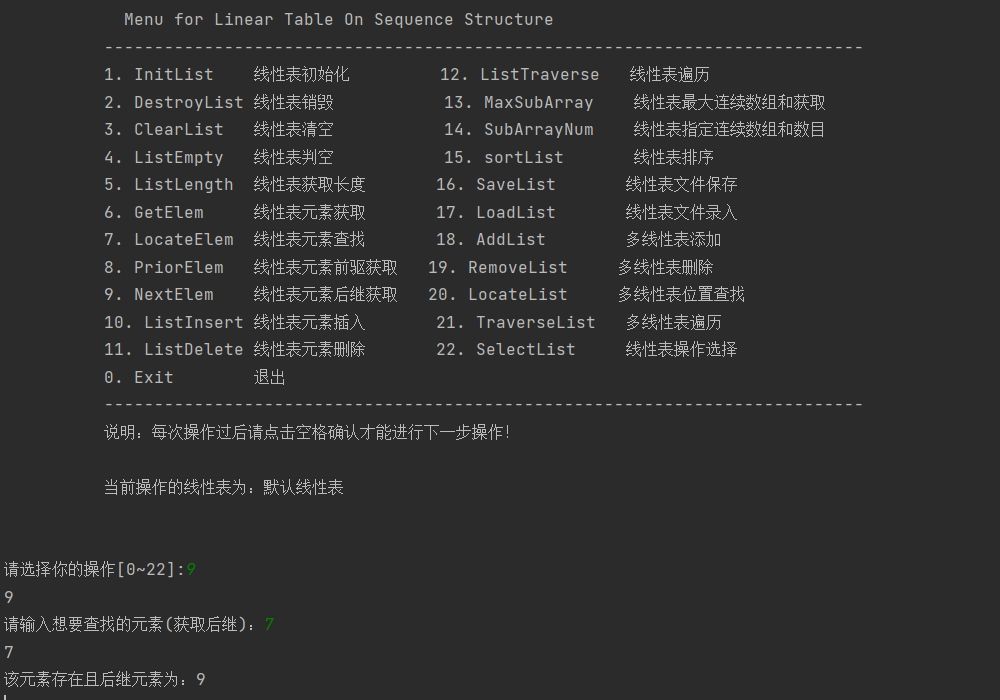
\includegraphics[width=0.6\textwidth]{images/线性表测试9.png}
 	\caption{测试2运行结果}
 	\label{txlab}
 \end{figure}


\paragraph{10.}ListInsert测试

	输入要求:依次输入插入元素位置和插入元素。

	测试1在空线性表的情况下进行,通过反复调用函数来构建测试集1(1 3 5 7 9),将通过遍历线性表和求表长来检验插入是否正确;

	测试2,3将在测试1的基础上进行,测试函数能否正确判断线性表两端非法的插入位置;

	测试4在测试集2的基础上进行,测试当线性表已满状态时,能否正确插入元素;

	测试5将在销毁线性表之后的情况下进行,测试函数能否正确判断线性表的存在性;

	测试6将在清空线性表之后的情况下进行,测试函数能否正确判断非法的插入位置。

\vspace{0.5em}

\begin{tabular}{|c|p{2.8cm}|p{5cm}|c|}
	\hline
	测试编号 & 测试输入 & 预期结果 & 实际运行结果 \\
	\hline
	1 & 10$\rightarrow$1 1$\rightarrow$10$\rightarrow$2 3$\rightarrow$10$\rightarrow$3 5$\rightarrow$10$\rightarrow$4 7$\rightarrow$10$\rightarrow$5 9 & 线性表插入成功! & 一致 \\
	\hline
	2 & 10$\rightarrow$7 & 插入位置不合法,线性表插入失败! & 一致 \\
	\hline
	3 & 10$\rightarrow$0 & 插入位置不合法,线性表插入失败! & 一致 \\
	\hline
	4 & 10$\rightarrow$测试集2$\rightarrow$10$\rightarrow$21 21 & 线性表插入成功! & 一致 \\
	\hline
	5 & 2$\rightarrow$10$\rightarrow$1 1 & 线性表不存在,插入失败! & 一致 \\
	\hline
	6 & 3$\rightarrow$10$\rightarrow$3 1 & 插入位置不合法,线性表插入失败! & 一致 \\
	\hline
\end{tabular}

~\

 \begin{figure}[H]
 	\centering
 	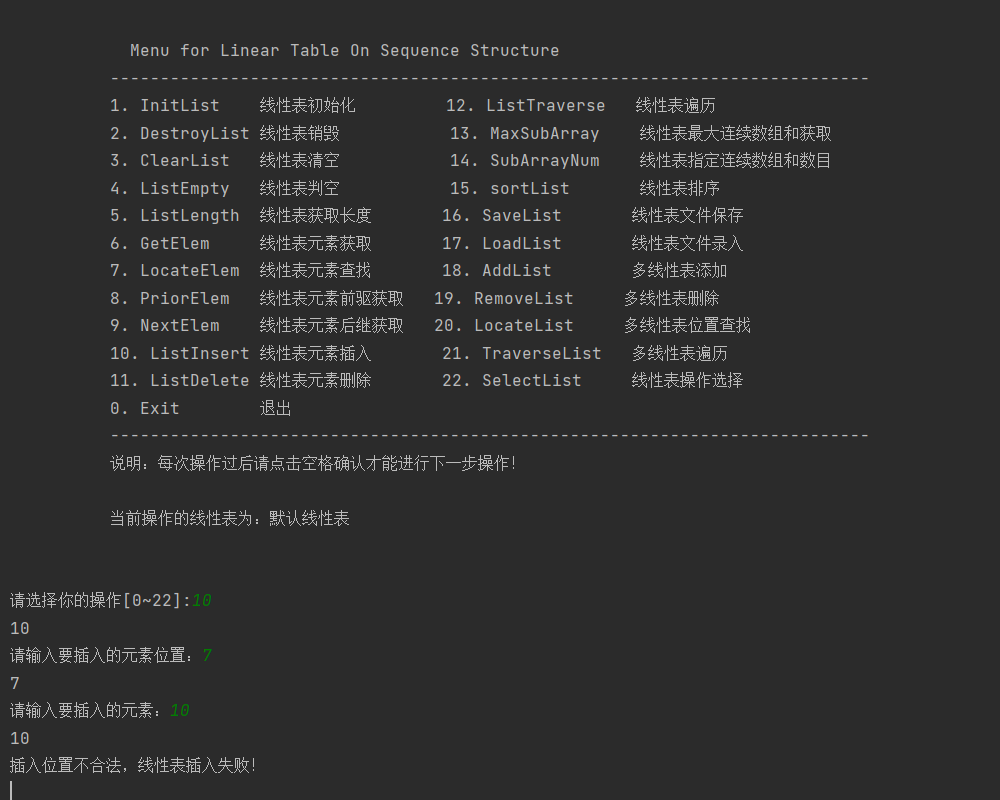
\includegraphics[width=0.6\textwidth]{images/线性表测试10.png}
 	\caption{测试2运行结果}
 	\label{txlab}
 \end{figure}


\paragraph{11.}ListDelete测试

	输入要求:输入删除的序号

	此函数的所有测试将在测试集1的情况下进行,进行一项测试后,不恢复至测试集1的状态。

	测试1:将测试函数能否正确判断非法的序号;

	测试2:将测试函数能否正确删除元素,采用遍历的方式检验正确性;

	测试3:在测试2的基础上完成,将测试函数能否正确删除元素,采用遍历和求表长的方式检验正确性;

\vspace{0.5em}

\begin{tabular}{|c|p{2.7cm}|p{4.5cm}|c|}
	\hline
	测试编号 & 测试输入 & 预期结果 & 实际运行结果 \\
	\hline
	1 & 11$\rightarrow$0 & 删除位置不合法! & 一致 \\
	\hline
	2 & 11$\rightarrow$2$\rightarrow$2 & 元素已删除!遍历后的结果为1 5 7 9 & 一致 \\
	\hline
	3 & 11$\rightarrow$1$\rightarrow$5 & 元素已删除!线性表的长度为3! & 一致 \\
	\hline
\end{tabular}

~\

 \begin{figure}[H]
 	\centering
 	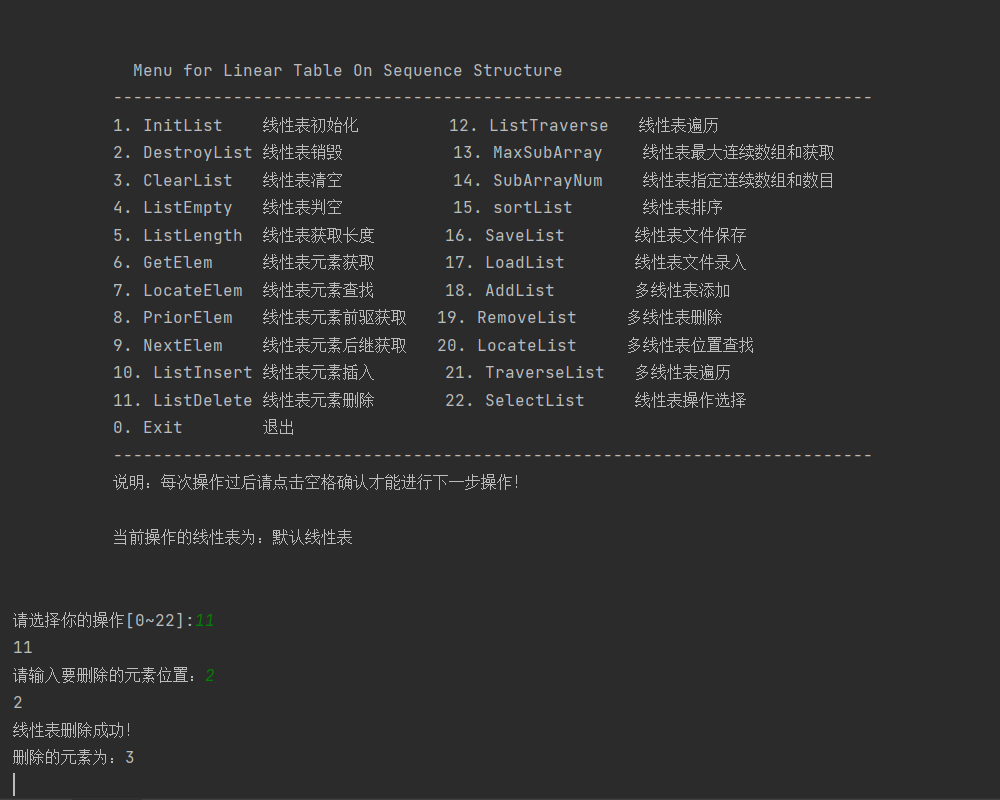
\includegraphics[width=0.6\textwidth]{images/线性表测试11.png}
 	\caption{测试2运行结果}
 	\label{txlab}
 \end{figure}


\paragraph{12.}ListTraverse测试

	测试1在没有创建线性表的情况下进行,测试函数能否正确判断线性表的存在性;

	测试2在线性表是空表的情况下进行,测试函数能否处理空表的情况;

	测试3在测试集1的情况下进行,测试函数能否正确遍历线性表。

\vspace{0.5em}

\begin{tabular}{|c|p{2.7cm}|c|c|}
	\hline
	测试编号 & 测试输入 & 预期结果 & 实际运行结果 \\
	\hline
	1 & 12 & 线性表不存在!不能遍历 & 一致 \\
	\hline
	2 & 3$\rightarrow$12 & 线性表是空表 & 一致 \\
	\hline
	3 & 12 & 1 3 5 7 9 & 一致 \\
	\hline
\end{tabular}

~\

 \begin{figure}[H]
 	\centering
 	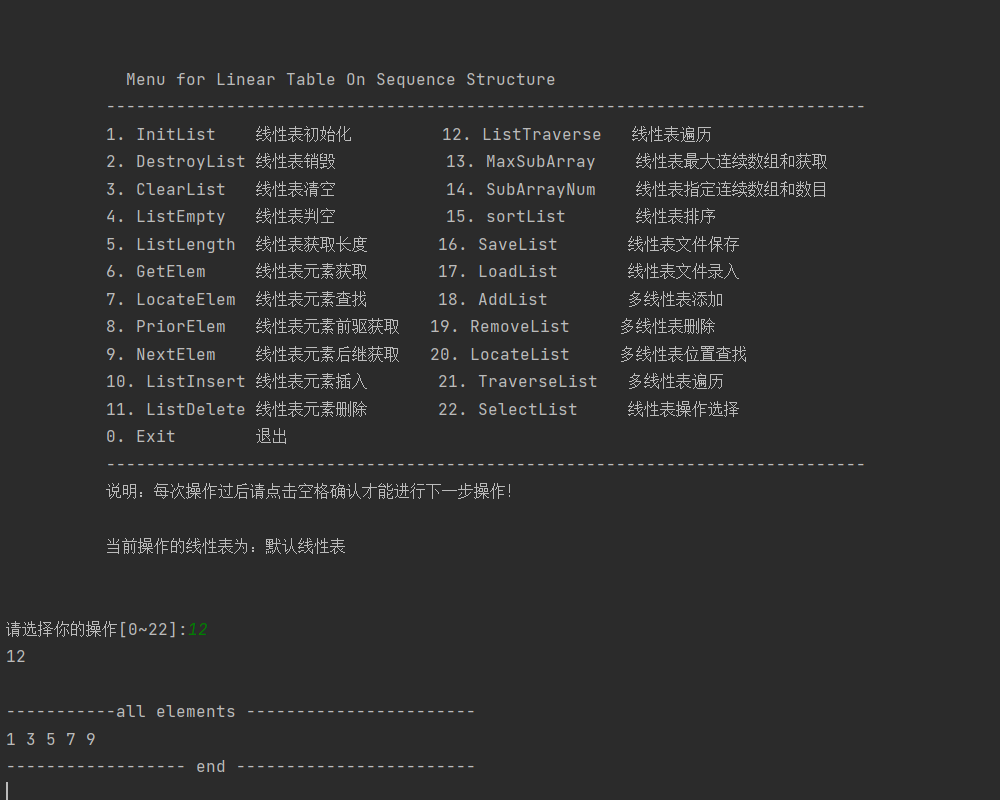
\includegraphics[width=0.6\textwidth]{images/线性表测试12.png}
 	\caption{测试3运行结果}
 	\label{txlab}
 \end{figure}


\subsubsection{附加功能测试}

\paragraph{13.}MaxSubArray测试

测试1:在没有创建线性表的情况下进行,测试函数能否正确判断线性表的存在性;
	
测试2:在测试集4的情况下进行,测试函数能否实现求最大连续子数组和的功能。

\vspace{0.5em}

\begin{tabular}{|c|p{2.7cm}|c|c|}
	\hline
	测试编号 & 测试输入 & 预期结果 & 实际运行结果 \\
	\hline
	1 & 2$\rightarrow$13 & 线性表未创建! & 一致 \\
	\hline
	2 & 13 & 最大子数组之和为: 6& 一致 \\
	\hline
\end{tabular}

~\

\paragraph{14.}SubArrayNum测试
	
测试1:在没有创建线性表的情况下进行,测试函数能否正确判断线性表的存在性;

测试2、3、4:在测试集4的情况下进行,测试函数能否实现计数和为K的子数组的功能。

\vspace{0.5em}

\begin{tabular}{|c|p{2.7cm}|c|c|}
	\hline
	测试编号 & 测试输入 & 预期结果 & 实际运行结果 \\
	\hline
	1 & 2$\rightarrow$14 & 线性表未创建! & 一致 \\
	\hline
	2 & 14$\rightarrow$3 & 和为数3的连续数组数目为:5 & 一致 \\
	\hline
	3 & 14$\rightarrow$5 & 和为数5的连续数组数目为:2 & 一致 \\
	\hline
	4 & 14$\rightarrow$7 & 和为数7的连续数组数目为:0 & 一致 \\
	\hline
\end{tabular}

~\

\paragraph{15.}sortList测试
	
测试1:在线性表为空的情况下进行,测试函数能否正确判断线性表为空;

测试2:在线性表不存在的情况下进行,测试函数能否正确排序。

\vspace{0.5em}

\begin{tabular}{|c|p{2.7cm}|c|c|}
	\hline
	测试编号 & 测试输入 & 预期结果 & 实际运行结果 \\
	\hline
	1 & 3$\rightarrow$15 & 线性表是空表! & 一致 \\
	\hline
	2 & 2$\rightarrow$15$\rightarrow$12 & -5 -3 -2 -1 1 1 2 4 4 & 一致 \\
	\hline
\end{tabular}

~\

\paragraph{16.}SaveList测试
	
测试1:在测试集1的情况下进行,测试函数能否正常进行写文件操作;

测试2:在文件已经有内容时,测试函数是否能够判断文件不能覆盖;

测试3:在线性表不存在的情况下进行,测试函数能否给出正确判断。

\vspace{0.5em}

\begin{tabular}{|c|p{2.7cm}|c|c|}
	\hline
	测试编号 & 测试输入 & 预期结果 & 实际运行结果 \\
	\hline
	1 & 16$\rightarrow$1.txt & 文件保存成功! & 一致 \\
	\hline
	2 & 16$\rightarrow$1.txt & 该文件已有内容,不能读入! & 一致 \\
	\hline
	3 & 2$\rightarrow$16$\rightarrow$1.txt & 线性表不存在!文件保存失败! & 一致 \\
	\hline
\end{tabular}

~\

\paragraph{17.}LoadList测试
	
本函数的测试都在文件1中已存有测试集1的情况下进行。

测试1:在线性表不存在的情况下进行,测试函数能否正确进行读文件操作,采用遍历线性表的方式检验正确性。

测试2:在线性表存在的情况下进行,测试函数能否给出正确判断。

\vspace{0.5em}

\begin{tabular}{|c|p{2.7cm}|c|c|}
	\hline
	测试编号 & 测试输入 & 预期结果 & 实际运行结果 \\
	\hline
	1 & 2$\rightarrow$17$\rightarrow$1.txt & 文件录入成功!遍历:1 3 5 7 9 & 一致 \\
	\hline
	2 & 17$\rightarrow$1.txt & 线性表存在!文件录入失败! & 一致 \\
	\hline
\end{tabular}

~\

\paragraph{18.}AddList测试

测试1:将测试函数能否正确添加线性表;

测试2:在测试1的基础上进行,当线性表表名重复时,测试函数能否给出正确的判断。

测试3:构建测试集3,测试线性表能否正确添加,通过遍历各个表检验正确性。

\vspace{0.5em}

\begin{tabular}{|c|p{2.7cm}|c|c|}
	\hline
	测试编号 & 测试输入 & 预期结果 & 实际运行结果 \\
	\hline
	1 & 18$\rightarrow$FirstList & FirstList已成功添加! & 一致 \\
	\hline
	2 & 18$\rightarrow$FirstList & 该名称的线性表已经存在! & 一致 \\
	\hline
	3 & 21 & FirstList SecondList & 一致 \\
	\hline
\end{tabular}

~\

\paragraph{19.}RemoveList测试

本函数的测试在测试集3的基础上进行。

测试1:将测试函数能否正确删除线性表,采用遍历各线性表的方式判断正确性;

测试2:在测试1的基础上进行,尝试删除一个不在集合中的线性表,测试函数能否给出正确判断。

\vspace{0.5em}

\begin{tabular}{|c|p{2.7cm}|c|c|}
	\hline
	测试编号 & 测试输入 & 预期结果 & 实际运行结果 \\
	\hline
	1 & 19$\rightarrow$FirstList & FirstList已成功删除! & 一致 \\
	\hline
	2 & 19$\rightarrow$ThirdList & 线性表不存在! & 一致 \\
	\hline
\end{tabular}

~\

\paragraph{20.}LocateList测试
	
本函数的测试在测试集3的基础上进行。

测试1:将测试函数能否正确定位线性表;

测试2:将尝试查找一个不在集合中的线性表,测试函数能否给出正确判断。

\vspace{0.5em}

\begin{tabular}{|c|p{2.7cm}|c|c|}
	\hline
	测试编号 & 测试输入 & 预期结果 & 实际运行结果 \\
	\hline
	1 & 20$\rightarrow$FirstList & 该线性表的逻辑索引为:1 & 一致 \\
	\hline
	2 & 20$\rightarrow$ThirdList & 线性表查找失败! & 一致 \\
	\hline
\end{tabular}

~\

\paragraph{21.}TraverseList测试
	
测试1:在测试集3的基础上进行,测试函数能否正确遍历各个线性表;

测试2:在空集合的基础上进行,测试函数能否给出正确判断。

\vspace{0.5em}

\begin{tabular}{|c|p{2.7cm}|c|c|}
	\hline
	测试编号 & 测试输入 & 预期结果 & 实际运行结果 \\
	\hline
	1 & (测试集3)21 & FirstList SecondList & 一致 \\
	\hline
	2 & 21 & 多线性表为空! & 一致 \\
	\hline
\end{tabular}

~\

\paragraph{22.}SelectList测试
	
输入要求:输入线性表集合中线性表对应的逻辑索引。
	
测试1,2:在测试集3的情况下进行,测试函数能否正确判断非法的位序;

测试3:在测试集3的情况下进行,测试函数能否正确地实现选取线性表操作。

\vspace{0.5em}

\begin{tabular}{|c|p{2.7cm}|c|c|}
	\hline
	测试编号 & 测试输入 & 预期结果 & 实际运行结果 \\
	\hline
	1 & 22$\rightarrow$0 & 线性表选取失败! & 一致 \\
	\hline
	1 & 22$\rightarrow$3 & 线性表选取失败! & 一致 \\
	\hline
	2 & 22$\rightarrow$1 & 线性表已选取成功! & 一致 \\
	\hline
\end{tabular}

~\

测试小结

22个函数基本符合了测试要求,在正常和异常用例的条件下均可以正常运行。需要注意的是,在对某些函数进行测试时,出于篇幅限制,没有测试线性表不存在的情况,同时对于附加功能函数没有具体给测试后的控制台界面。

\subsection{实验小结}

本次实验让我加深了对线性表的概念、基本运算的理解,掌握了线性表的基本运算的实现,熟练了线性表的逻辑结构和物理结构的关系。

在编写程序和测试的过程中,遇到了诸多问题,例如如何设计多线性表操作,如何保证能够单独对某一线性表进行基本操作。解决方案是将其完整赋值给主函数中的
全局变量,保证了集合中表的独立性,可以不受主函数中操作的影响,表之间可以分立进行。

在今后的学习过程当中应该更多地从数据结构的角度去分析如何进行数据的存储、读取和处理,如何设计便于存储的数据结构,同时应具有开放性思维,设计高性能的算法,以达到更简便地解决实际问题的目的。同时,以后还需要多加练习,以达到熟能生巧的效果。


\newpage

\section{基于二叉链表的二叉树实现}

\subsection{问题描述}

采用二叉链表作为二叉树的物理结构,实现基本运算。ElemType为数据元素的类型名,具体含义可自行定义,但要求二叉树结点类型为结构型,至少包含二个部分,一个是能唯一标识一个结点的关键字(类似于学号或职工号),另一个是其它部分。其它有关类型和常量的定义和引用详见文献[1]的p10。

要求构造一个具有菜单的功能演示系统。其中,在主程序中完成函数调用所需实参值的准备和函数执行结果的显示,并给出适当的操作提示显示。

演示系统可选择实现二叉树的文件形式保存。其中,\whiteding{1}需要设计文件数据记录格式,以高效保存二叉树数据逻辑结构(D,{R})的完整信息;\whiteding{2}需要设计二叉树文件保存和加载操作合理模式。附录B提供了文件存取的方法。
演示系统可选择实现多个二叉树管理。可采用线性表的方式管理多个二叉树,线性表中的每个数据元素为一个二叉树的基本属性,至少应包含有二叉树的名称。基于顺序表实现的二叉树管理,其物理结构的参考设计如图3-1所示。

\begin{figure}[htbp] % here top bottom
    \vspace{0.8cm}
	\begin{center}
		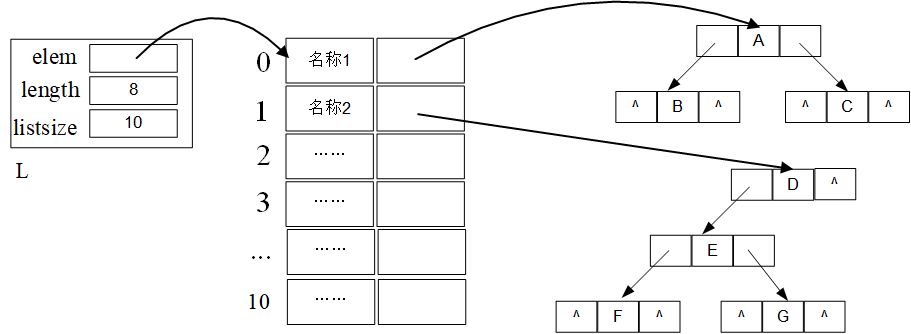
\includegraphics[scale=0.7]{images/二叉树物理结构.png}
		\caption{二叉树物理结构示意图}
		\label{fig1-1}
	\end{center}
\end{figure}

演示系统的源程序应按照代码规范增加注释和排版,目标程序务必是可以独立于IDE运行的EXE文件。

\subsection{系统设计}

\subsubsection{头文件和预定义}

1、头文件

\begin{lstlisting}[language=c]
#include <stdio.h>
#include <stdlib.h>
#include <string.h>
#include <windows.h>
\end{lstlisting}

2、预定义常量

\begin{lstlisting}[language=c]
#define TRUE 1
#define FALSE 0
#define OK 1
#define ERROR 0
#define INFEASIBLE -1
#define OVERFLOW -2
#define MAXlength 10

\end{lstlisting}

3、类型表达式

\begin{lstlisting}[language=c]
typedef int status;
typedef int KeyType;
typedef struct {
    KeyType  key;
    char others[20];
} TElemType; //二叉树结点类型定义

typedef struct BiTNode{  //二叉链表结点的定义
    TElemType  data;
    struct BiTNode *lchild,*rchild;
} BiTNode, *BiTree;

typedef struct{  //线性表的集合类型定义
    struct { char name[30];
        BiTree L;
    } elem[11];
    int length;
}TREES;
TREES trees;      //线性表集合的定义TREES
\end{lstlisting}

\subsubsection{基本功能函数}

 \begin{figure}[H]
 	\centering
 	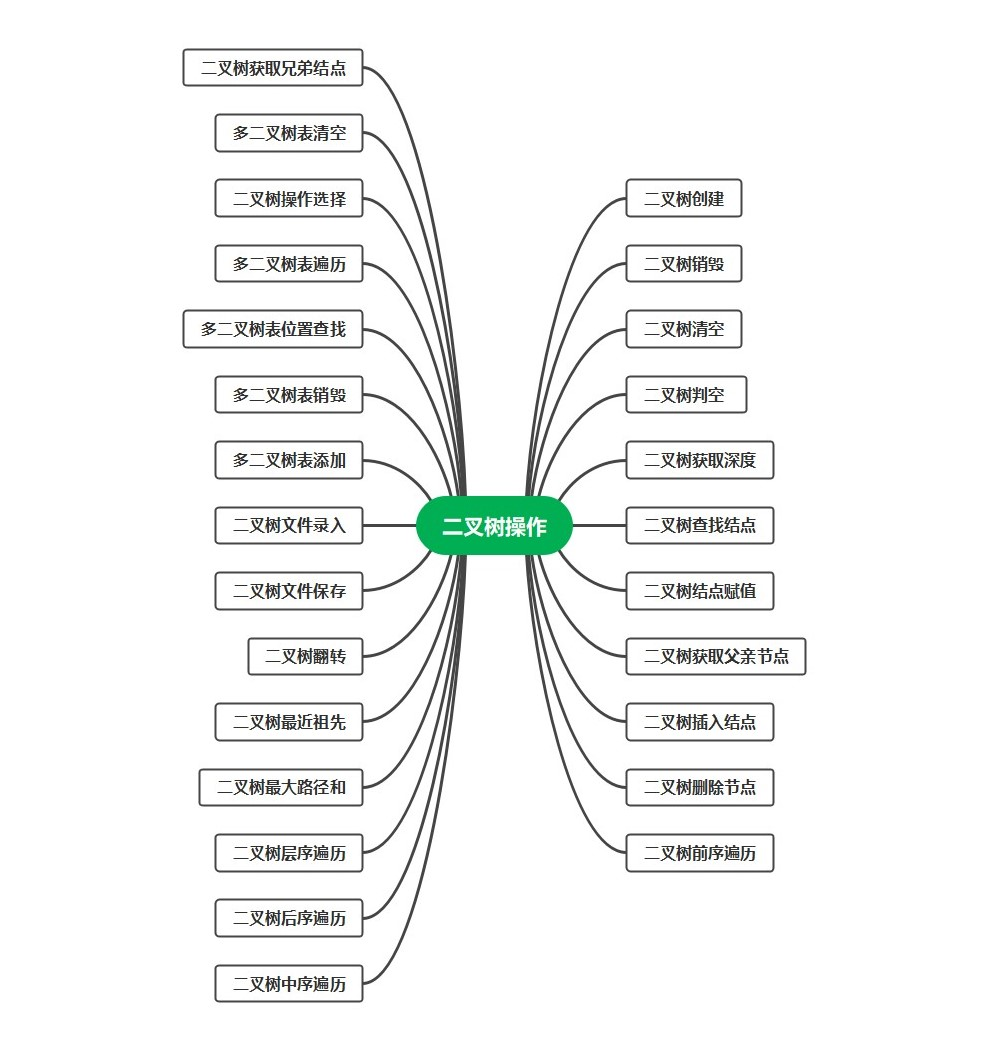
\includegraphics[width=0.9\textwidth]{images/二叉树操作.jpg}
 	\caption{系统整体功能设计图}
 	\label{txlab}
 \end{figure}

二叉树的逻辑结构如下:

ADT Tree \{

数据对象  $\mathrm{D}$: $\mathrm{D}$  是具有相同特性的数据元素的集合。

数据关系  R:  若  D  为空集, 则称为空树;

若  D  仅含一个数据元素, 则  R  为空集, 否则  R=\{H\}, H  是如下二元关系:

(1) 在 D 中存在惟一的称为根的数据元素 root, 它在关系  $\mathrm{H}$  下无前驱;

(2) 若  D - \{root\} $\neq \Phi$ , 则存在   D - \{root\}  的一个划分  $\mathrm{D}_{1}$, $\mathrm{D}_{2}$, $\cdots$, $\mathrm{D}_{m}$ $(\mathrm{m}>0)$ , 对任意  j $\neq$ k (1 $\leq$   j, k $\leq$ m)  有  $\mathrm{D}_{j}$ $\cap$ $\mathrm{D}_{k}$=$\Phi$ , 且对任意的  i (1 $\leq$ i $\leq$ m) , 惟一存在数据元素  $\mathrm{x}_{i}$ $\in$ $\mathrm{D}_{i}$ , 有  <root, $\mathrm{x}_{i}$> $\in$ $\mathrm{H}$ ;

(3) 对应于 D-\{root\}  的划分,  H - <root, $\mathrm{x}_{1}$>,$\cdots$,<root, $\mathrm{x}_{0}$>有惟一的一个划分  $\mathrm{H}_{1}$,$\mathrm{H}_{2}$, $\cdots$, $\mathrm{H}_{m}$ $(\mathrm{m}>0)$ , 对任意  j $\neq$ k (1 $\leq$ j, k $\leq$ m)  有  $\mathrm{H}_{j}$ $\cap$ $\mathrm{H}_{k}$=$\Phi$ , 且对任意  i (1 $\leq$ i $\leq$ m), $\mathrm{H}_{i}$  是  $\mathrm{D}_{i}$  上的二元关系,  $\left(\mathrm{D}_{i},\left\{\mathrm{H}_{i}\right\}\right)$  是一棵符合本定义的树, 称为根 root 的子树。

\}

依据最小完备性和常用性相结合的原则,以函数形式定义了二叉树的创建二叉树、销毁二叉树、清空二叉树、判定空二叉树和求二叉树深度等14种基本运算。具体运算功能定义和说明如下:

\begin{enumerate}
    \item 创建二叉树:函数名称是CreateBiTree(T,definition);初始条件是definition 给出二叉树T的定义,如带空子树的二叉树前序遍历序列、或前序+中序、或后序+中序;操作结果是按definition构造二叉树T;

注:\whiteding{1}要求T中各结点关键字具有唯一性。后面各操作的实现,也都要满足一棵二叉树中关键字的唯一性,不再赘述;\whiteding{2}CreateBiTree中根据definition生成T,不应在CreateBiTree中输入二叉树的定义。
    \item 销毁二叉树:函数名称是DestroyBiTree(T);初始条件是二叉树T已存在;操作结果是销毁二叉树T;
    \item 清空二叉树:函数名称是ClearBiTree (T);初始条件是二叉树T存在;操作结果是将二叉树T清空;
    \item 判定空二叉树:函数名称是BiTreeEmpty(T);初始条件是二叉树T存在;操作结果是若T为空二叉树则返回TRUE,否则返回FALSE;
    \item 求二叉树深度:函数名称是BiTreeDepth(T);初始条件是二叉树T存在;操作结果是返回T的深度;
    \item 查找结点:函数名称是LocateNode(T,e);初始条件是二叉树T已存在,e是和T中结点关键字类型相同的给定值;操作结果是返回查找到的结点指针,如无关键字为e的结点,返回NULL;
    \item 结点赋值:函数名称是Assign(T,e,value);初始条件是二叉树T已存在,e是和T中结点关键字类型相同的给定值;操作结果是关键字为e的结点赋值为value;
	\item 获得兄弟结点:函数名称是GetSibling(T,e);初始条件是二叉树T存在,e是和T中结点关键字类型相同的给定值;操作结果是返回关键字为e的结点的(左或右)兄弟结点指针。若关键字为e的结点无兄弟,则返回NULL;
	\item 插入结点:函数名称是InsertNode(T,e,LR,c);初始条件是二叉树T存在,e是和T中结点关键字类型相同的给定值,LR为0或1,c是待插入结点;操作结果是根据LR为0或者1,插入结点c到T中,作为关键字为e的结点的左或右孩子结点,结点e的原有左子树或右子树则为结点c的右子树;

特殊情况,c插入作为根结点,可以考虑LR为-1时,作为根结点插入,原根结点作为c的右子树。
	\item 删除结点:函数名称是DeleteNode(T,e);初始条件是二叉树T存在,e是和T中结点关键字类型相同的给定值。操作结果是删除T中关键字为e的结点;同时,如果关键字为e的结点度为0,删除即可;如关键字为e的结点度为1,用关键字为e的结点孩子代替被删除的e位置;如关键字为e的结点度为2,用e的左孩子代替被删除的e位置,e的右子树作为e的左子树中最右结点的右子树;
	\item 前序遍历:函数名称是PreOrderTraverse(T,Visit());初始条件是二叉树T存在,Visit是一个函数指针的形参(可使用该函数对结点操作);操作结果:先序遍历,对每个结点调用函数Visit一次且一次,一旦调用失败,则操作失败。

注:前序、中序和后序三种遍历算法,要求至少一个用非递归算法实现。

	\item 中序遍历:函数名称是InOrderTraverse(T,Visit));初始条件是二叉树T存在,Visit是一个函数指针的形参(可使用该函数对结点操作);操作结果是中序遍历t,对每个结点调用函数Visit一次且一次,一旦调用失败,则操作失败;
	\item 后序遍历:函数名称是PostOrderTraverse(T,Visit));初始条件是二叉树T存在,Visit是一个函数指针的形参(可使用该函数对结点操作);操作结果是后序遍历t,对每个结点调用函数Visit一次且一次,一旦调用失败,则操作失败。
	\item 按层遍历:函数名称是LevelOrderTraverse(T,Visit));初始条件是二叉树T存在,Visit是对结点操作的应用函数;操作结果是层序遍历t,对每个结点调用函数Visit一次且一次,一旦调用失败,则操作失败。
\end{enumerate}

\subsubsection{附加功能函数}

\begin{enumerate}
    \item 最大路径和:函数名称是MaxPathSum(T),初始条件是二叉树T存在;操作结果是返回根节点到叶子结点的最大路径和;
    \item 最近公共祖先:函数名称是LowestCommonAncestor(T,e1,e2);初始条件是二叉树T存在;操作结果是该二叉树中e1节点和e2节点的最近公共祖先;
    \item 翻转二叉树:函数名称是InvertTree(T),初始条件是线性表L已存在;操作结果是将T翻转,使其所有节点的左右节点互换;
    \item 实现线性表的文件形式保存:其中,\whiteding{1}需要设计文件数据记录格式,以高效保存线性表数据逻辑结构(D,{R})的完整信息;\whiteding{2}需要设计线性表文件保存和加载操作合理模式。
	\begin{enumerate}
	\item 文件写入:函数名称是 SaveList(T,FileName);初始条件是二叉树T已存在;操作结果是将T的元素写到名称为FileName的文件中。
	\item 文件读出:函数名称是 LoadList(T,FileName);初始条件是二叉树T不存在;操作结果是将文件 FileName 中的元素读到表 T中。
	\end{enumerate}
    \item 实现多个二叉树管理:设计相应的数据结构管理多个二叉树的查找、添加、移除等功能。
	\begin{enumerate}
	\item 增加二叉树:函数名称是 AddList(trees, ListName);初始条件是名称为ListName的二叉树不存在于二叉树集合中;操作结果是在 Lists中创建一个名称为ListName 的初始化好的线性表。
	\item 移除二叉树:函数名称是RemoveList(trees, ListName);初始条件是名称为ListName的二叉树存在于二叉树集合中;操作结果是将该线性表移除。
	\item 查找二叉树:函数名称是LocateList(trees, ListName);初始条件是名称为ListName的二叉树存在于二叉树集合中;操作结果是返回该二叉树在Lists中的逻辑索引。
	\item 遍历所有表:函数名称是TraverseList(trees,visit());初始条件是trees已存在;操作结果是对所有的表遍历并输出。
	\item 选择表:函数名称是 SelectList (trees, i);初始条件是trees已存在,1≤i≤trees.Length+1;操作结果是将treea中逻辑索引为i的二叉树选择为当前处理的二叉树,以便后续再调用其他函数对该树进行操作。
	\end{enumerate}
\end{enumerate}

\subsubsection{演示系统}

构造一个具有菜单的功能演示系统。其中,在主程序中完成函数调用所需实参值的准备和函数执行结果的显示,并给出适当的操作提示显示。演示系统可选择实现二叉树的文件形式保存。其中,\whiteding{1}需要设计文件数据记录格式,以高效保存二叉树数据逻辑结构(D,[R])的完整信息;\whiteding{2}需要设计二叉树文件保存和加载操作合理模式。演示系统实现了多个二叉树管理。
    输入1$\sim$26可以调用上述的26个函数,对二叉树或二叉树集合进行操作;输入0时退出系统。

该演示系统具有完备性,包含每一功能的中英文说明和注意事项,同时显示当前二叉树名称和初始化情况。

输入1$\sim$ 26可以调用上述的26个函数,对线性表或多线性表进行操作;输入0时退出系统。

\subsection{系统实现}

\subsubsection{演示系统框架}

系统主体通过while循环实现多次选择,通过op获取用户的选择,通过switch语句根据用户选择实现具体功能,通过system("cls")语句实现清屏操作,保证界面整洁和满足用户体验感。

具体实现为将菜单和功能实现写入到 while 循环中,用op 获取用户的选择,op初始化为 1,以便第一次能进入循环。进入循环后,用户输入选择 0$\sim$26,其中 1$\sim$26 分别代表二叉树的一个基本运算,在主函数中通过 switch语句对应到相应的函数功能,执行完该功能后通过 break 跳出switch 语句,继续执行 while 循环,直至用户输入 0 退出当前演示系统。系统初进入时默认对默认二叉树(未创建)进行操作,后续可增加新树并进行选择,实现森林的操作。

\subsubsection{数据结构设计}

\begin{enumerate}
	\item 二叉树:二叉树中用特殊类型data储存数据,其中数据包含关键元素key和关键信息others,定义BiTNode类型的lchild用于指向左子树结点,rchild用于指向右子树结点。
	\item 多二叉树的管理表:定义length变量表示管理二叉树表的长度。定义elem数组顺序储存二叉树及其名称。
	\end{enumerate}

\subsubsection{函数思想及实现}

\textbf{说明:无特殊说明情况下,每一函数均需判断二叉树是否存在之后,再对二叉树进行相应的操作。}

\setcounter{paragraph}{0}

二叉树基本功能函数的实现:

\paragraph{ 1.} status CreateBiTree(BiTree \&T, TElemType definition[])

输入:二叉树根结点,TELemType类型数组

输出:函数运行状态

函数思想描述:将创建二叉树写成函数,其中传入函数的参数是二叉树根节点和TELemType类型数组。根据带空枝的二叉树先根
遍历序列definition 构造一棵二叉树,将根节点指针赋值给 T 并返回 OK,若关键字不唯一就返回 ERROR。在函数中,首先调用函数checkKey判断输入的关键字是否唯一。然后对于 definition 中的结点,若关键字为-1 则创建结束;若关键字为 0,则当前子树创建结束;若关键字大于 0,则创建当前结点,并递归调用本函数依次创建本结点的左子树和右子树,最后创建完好的二叉树。

\paragraph{ 2.} status DestroyBiTree(BiTree \&T)
    
输入:二叉树根结点

输出:函数运行状态

函数思想描述:将清空二叉树写成函数,其中传入函数的参数是二叉树根节点指针。将二叉树设置成空,并删除所有结点,释放结点空间。在函数中,如果当前结点有左子树或右子树,则递归调用本函数依次清空当前结点的左子树和右子树;如果当前结点的左右子树都为空指针时释放当前结点的存储空间,并将当前结点的指针设置为 NULL。

\paragraph{ 3.}status ClearBiTree(BiTree \&T)
    
输入:二叉树根结点

输出:函数运行状态

函数思想描述:将销毁二叉树写成函数,其中传入函数的参数是二叉树根节点指针。将二叉树设置成空,并删除所有结点,释放结点空间。在函数中,如果当前结点有左子树或右子树,则递归调用本函数依次清空当前结点的左子树和右子树;如果当前结点的左右子树都为空指针时释放当前结点的存储空间,并将当前结点的指针设置为 NULL,操作基本与销毁相同,除非包含头结点指向二叉树的根。

\paragraph{ 4.}status BiTreeEmpty(BiTree T)

输入:二叉树根结点

输出:函数运行状态

函数思想描述:判断树的根结点是否存在,如果结点为空,则返回FALSE,否则说明树非空,返回TRUE。

\paragraph{ 5.}int BiTreeDepth(BiTree T)

输入:二叉树根结点

输出:整型变量(含义为二叉树深度)

函数思想概述:将求二叉树深度写成函数,其中传入函数的参数是二叉树根节点指针。依次遍历二叉树的左右结点,遇到空结点则返回0,不断比较获取二叉树到叶子结点的长度的最大值,作为二叉树的深度。

\paragraph{ 6.}BiTNode *LocateNode(BiTree T, KeyType e)

输入:二叉树根结点,KeyType类型(查找结点的关键字)

输出:二叉树结点指针

函数思想描述:将查找二叉树中关键字为特定值的结点写成函数,其中传入函数的参数是二叉树根结点指针和查找结点的关键字。该函数使用递归思想,若当前结点为目标结点,则返回当前结点的地址值;若当前结点指针为空,则说明此子树都没有所找结点,返回 NULL 指针;否则依次递归查找左右子树中是否有目标结点,并记录在左右子树查找的返回值。整个函数的返回值若为NULL,则说明整棵树没有目标结点,否则返回目标结点。

\paragraph{ 7.}status Assign(BiTree \&T, KeyType e, TElemType value)

输入:二叉树根结点,KeyType类型(查找结点的关键字),TElemType类型变量(存储要替代的结点信息)

输出:函数运行状态

函数思想描述:将实现结点赋值写成函数,其中传入函数的参数是二叉树根结点指针、查找结点的关键字、用以替换的结点值。在函数中,首先通过 LocateNode 函数查找用以替换的结点的关键字与除被替换结点以外的其他结点的关键字是否有重复,若重复则返回 ERROR。若无重复则调用 LocateNode 函数查找被替换结点,若未找到则返回 ERROR;若找到,则对该结点的关键字和关键信息进行赋值,并返回OK。

\paragraph{ 8.}BiTNode *GetSibling(BiTree T, KeyType e)

输入:二叉树根结点,KeyType类型(查找结点的关键字)

输出:二叉树结点指针

函数思想概述:将获得当前结点的兄弟结点写成函数。该函数使用了递归思想。在函数中,若当前结点为空则说明为空树,若当前结点无左右子树则说明当前结点不符合条件,返回 NULL;若当前结点有左右子树,则若左右子树其一结点关键字为所求,且另一子树存在,则找到兄弟结点,返回兄弟结点指针,若另一子树不存在,则该节点没有兄弟结点,返回 NULL;若当前结点的左右子树都不为指定节点,则递归调用此函数在左右子树中查找,并记录返回结果。整个函数若最终返回值为NULL 则说明该树没有此结点或此结点无兄弟节点;若返回值不为 NULL 则说明在某一子树中找到了指定节点的兄弟结点,返回该结点的值。

\paragraph{ 9.}status InsertNode(BiTree \&T, KeyType e, int LR, TElemType c)

输入:二叉树根结点,KeyType类型(待插入结点的关键字),整型变量(标志插入左子树或右子树),TElemType类型变量(存储要插入的结点信息)

输出:函数运行状态

函数思想概述:将插入结点写成函数。在函数中,首先通过LocateNode 函数判断待插入结点在树中有无关键字重复,若有则返回 ERROR,若无重复则调用 LocateNode 函数查找被插入结点,然后根据 LR 为 0 或者 1,插入结点 c 到 T 中,作为关键字为 e 的结点的左或右孩子结点,结点 e 的原有左子树或右子树则为结点 c 的右子树,返回 OK。如果插入失败,返回 ERROR。特别地,当 LR 为-1 时,作为根结点插入,原根结点作为 c 的右子树,最后返回 OK。

\paragraph{10.}status DeleteNode(BiTree \&T, KeyType e)

输入:二叉树根结点,KeyType类型(待删除结点的关键字)

输出:函数运行状态

函数思想概述:将删除结点写成函数。e 是和 T 中结点关键字类型相同的给定值。删除 T 中关键字为 e 的结点;如果关键字为 e 的结点度为 0,删除即可;如关键字为 e 的结点度为 1,用关键字为 e 的结点孩子代替被删除的 e 位置;如关键字为 e 的结点度为 2,用 e 的左孩子代替被删除的 e 位置,e 的右子树作为 e 的左子树中最右结点的右子树。成功删除结点后返回 OK,否则返回ERROR。

\paragraph{11.}status PreOrderTraverse(BiTree T, void (*visit)(BiTree))

输入:二叉树根结点,函数指针

输出:函数运行状态

函数思想概述:将先序遍历树写成函数。该函数采用了递归思想。在函数中,若当前结点为空,则返回 ERROR;若当前结点不为空,则首先通过visit访问当前结点,然后递归调用本函数先序遍历当前结点的左子树和右子树。

\paragraph{12.}status InOrderTraverse(BiTree T, void (*visit)(BiTree))

输入:二叉树根结点,函数指针

输出:函数运行状态

函数思想概述:将中序遍历树写成函数。该函数用非递归形式实现,调用栈的数据结构和相应操作函数。在函数中,首先定义和初始化栈,并定义 p为根节点指针。然后进行遍历左子树循环:若 p 不为空树,则将根指针进栈,此时若栈满返回 ERROR,若成功进栈则将 t 移向左子树。若该结点为空表示以栈顶元素为根节点的子树的左子树遍历结束。然后,若栈非空,则弹出栈,并访问该指针,再将该指针移向右子树,循环进行上述操作。此项工作一直循环到栈空且指针 p 为空,这表示无父节点未访问且无右子树未遍历。最终返回 OK。

\paragraph{13.}status PostOrderTraverse(BiTree T, void (*visit)(BiTree))

输入:二叉树根结点,函数指针

输出:函数运行状态

函数思想概述:将后序遍历树写成函数。该函数采用了递归思想。在函数中,若当前结点为空,则返回 ERROR;若当前结点不为空,则首先递归调用本函数依次后序遍历当前结点的左子树和右子树,然后访问当前结点。

\paragraph{14.}status LevelOrderTraverse(BiTree T, void (*visit)(BiTree))

输入:二叉树根结点,函数指针

输出:函数运行状态

函数思想概述:将层序遍历树写成函数。该函数用非递归形式实现,调用队列数据结构和相应操作函数。在函数中,首先定义并初始化队列,然后定义 p 为根节点,并将根结点进队列。然后开始循环,该循环在队列为空时结束:首先将根节点出队列,若此节点不为空则访问该结点并依次将该结点的左右子树进队列,该循环结束则说明已经遍历完所有结点。在队列中,根节点下一层的子树先进队列。再依此顺序将左右子树的下一层子树再进队列,以此类推,直到最后一层子树。所以在每一层内的遍历顺序为从左向右。

附加功能函数的实现:

\paragraph{15.}int MaxPathSum(BiTree T)

输入:二叉树根结点

输出:整型变量(含义为最大路径和)

函数思想描述:函数实现返回最大路径和的功能。该函数通过不断递归到叶子节点到空树返回ERROR,然后返回路径上的最大值,程序流程图如下:

 \begin{figure}[H]
 	\centering
 	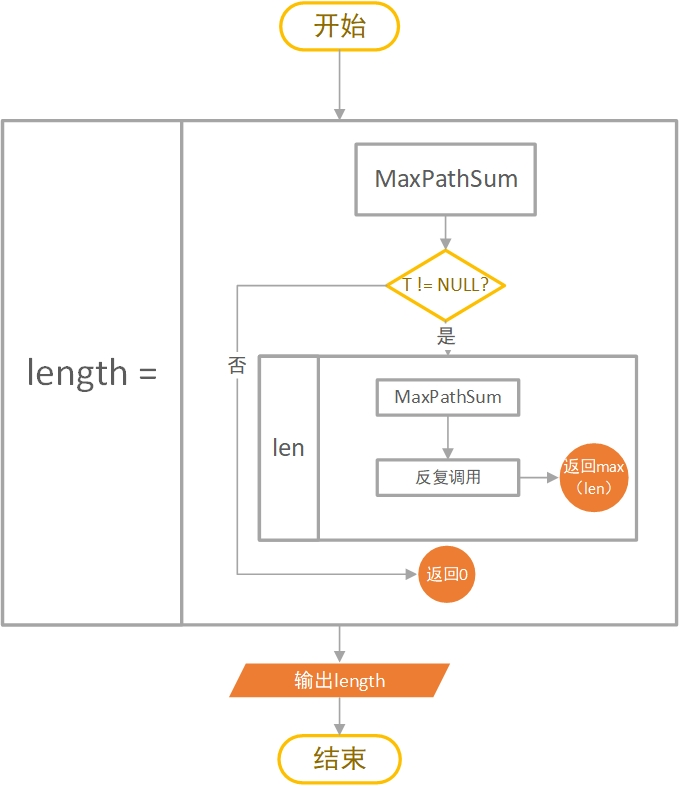
\includegraphics[width=0.7\textwidth]{images/最大流程.jpg}
 	\caption{MaxPathSum函数程序流程图}
 	\label{txlab}
 \end{figure}

时间复杂度:O(nlogn)

空间复杂度:O(n)

\paragraph{16.}BiTree LowestCommonAncestor(BiTree T, int e1, int e2)

输入:二叉树根结点,整型变量1(查找结点的关键字),整型变量2(查找结点的关键字)

输出:二叉树结点指针(含义为最近公共祖先)

函数思想描述:递归查找左子树和右子树,若查找到目标结点,则返回该结点的指针,若查找到空树,则返回NULL。然后判断若左结点的返回值和右节点的返回值均不为NULL,则返回该结点,若左结点和右节点存在一个结点不为空,则返回该结点;否则返回NULL。最终返回的结点为两结点的最近公共祖先。

时间复杂度:O(nlogn)

空间复杂度:O(n)

\paragraph{17.}status InvertTree(BiTree \&T)

输入:二叉树根结点

输出:函数运行状态

函数思想描述:将二叉树翻转写成函数。该函数用非递归形式实现,调用队列数据结构和相应操作函数。在函数中,首先定义并初始化队列,然后定义 p 为根节点,并将根结点进队列。然后开始循环,该循环在队列为空时结束:首先将根节点出队列,若此节点不为空则访问该结点并交换左右子树,然后依次将该结点的左右子树进队列,该循环结束则说明已经遍历完所有结点。最终得到翻转后的二叉树。

时间复杂度:O(n)

空间复杂度:O(n)

\paragraph{18.}status SaveBiTree(BiTree T, char FileName[])

输入:二叉树根结点,字符串变量

输出:函数运行状态

函数思想描述:将把树写入文件写成函数,将二叉树的结点数据写入到文件 FileName 中。该函数采用了非递归思想,通过栈的数据结构模拟先序遍历带空枝遍历,并将遍历结果写入文件中。

\paragraph{19.}status LoadBiTree(BiTree \&T,  char FileName[])

输入:二叉树根结点,字符串变量

输出:函数运行状态

函数思想描述:将从文件中读取树写成函数,将文件 FileName 中的数据读取到空树中,该函数采用了递归思想,该函数是将读取的数据按照先序遍历带空枝遍历对空树进行赋值的。

\paragraph{20.}status AddList(TREES \&trees,char ListName[])

输入:结构体类型变量(森林),字符串类型(含义为待添加树的名称)

输出:函数运行状态

函数思想描述:将增加树写成函数,函数的参数是森林和树名称。trees是一个以数组形式管理的森林,在数组尾部新增树,并将树名称存储在该树结点的 name 分量当中。当然,在添加二叉树之前,应当判断名称是否唯一。

\paragraph{21.}status DestoryList(TREES \&trees,char ListName[])

输入:结构体类型变量(森林),字符串类型(含义为待删除树的名称)

输出:函数运行状态

函数思想描述:将树写销毁树成函数,函数的参数是森林和树名称。在 trees数组中查找名称为 ListName 的树,查找成功则将其删除,否则返回ERROR。

\paragraph{22.}int LocateList(TREES trees,char ListName[])

输入:结构体类型变量(森林),字符串类型(含义为待查找树的名称)

输出:整型变量(二叉树的位序)

函数思想描述:将查找二叉树写成函数,函数的参数是森林和树名称。在 trees数组中查找名称为 ListName 的树,查找成功返回其位序。

\paragraph{23.}status TraverseList(TREES trees)

输入:结构体类型变量(森林)

输出:函数运行状态

函数思想描述:将遍历森林写成函数,函数的参数为森林。顺序遍历森林中各个树即可。

\paragraph{24.}status SelectList(TREES trees, int i)

输入:结构体类型变量(森林),整型变量(含义为逻辑索引)

输出:函数运行状态

函数思想描述:将选择二叉树写成函数,函数的参数为森林和逻辑索引。将Trees中逻辑索引为i的树赋值给主函数中的树T,后续可调用其他函数将对此二叉树进行操作。

\paragraph{25.}status ClearList(BiTree \&T)

输入:二叉树根结点

输出:函数运行状态

函数思想描述:将清空在森林中的二叉树写成函数。直接调用ClearBiTree函数清空二叉树,保留二叉树的位置和名称。

\paragraph{26.}BiTNode* GetFabling(BiTree T,KeyType e)

输入:二叉树根结点,KeyType类型(查找结点的关键字)

输出:二叉树结点指针

函数思想概述:将获得当前结点的父亲结点写成函数。该函数使用了递归思想。在函数中,若当前结点为空则说明为空树,若当前结点无左右子树则说明当前结点不符合条件,返回 NULL;若当前结点有左右子树,则若左右子树其一结点关键字为所求,则找到父亲结点,返回父亲结点指针。若当前结点的左右子树都不为指定节点,则递归调用此函数在左右子树中查找,并记录返回结果。整个函数若最终返回值为NULL,则说明该树没有此结点或此结点无父亲节点;若返回值不为 NULL 则说明在某一子树中找到了指定节点的父亲结点,返回该结点的值。

\subsection{系统测试}

系统菜单整体布局如图:

 \begin{figure}[H]
 	\centering
 	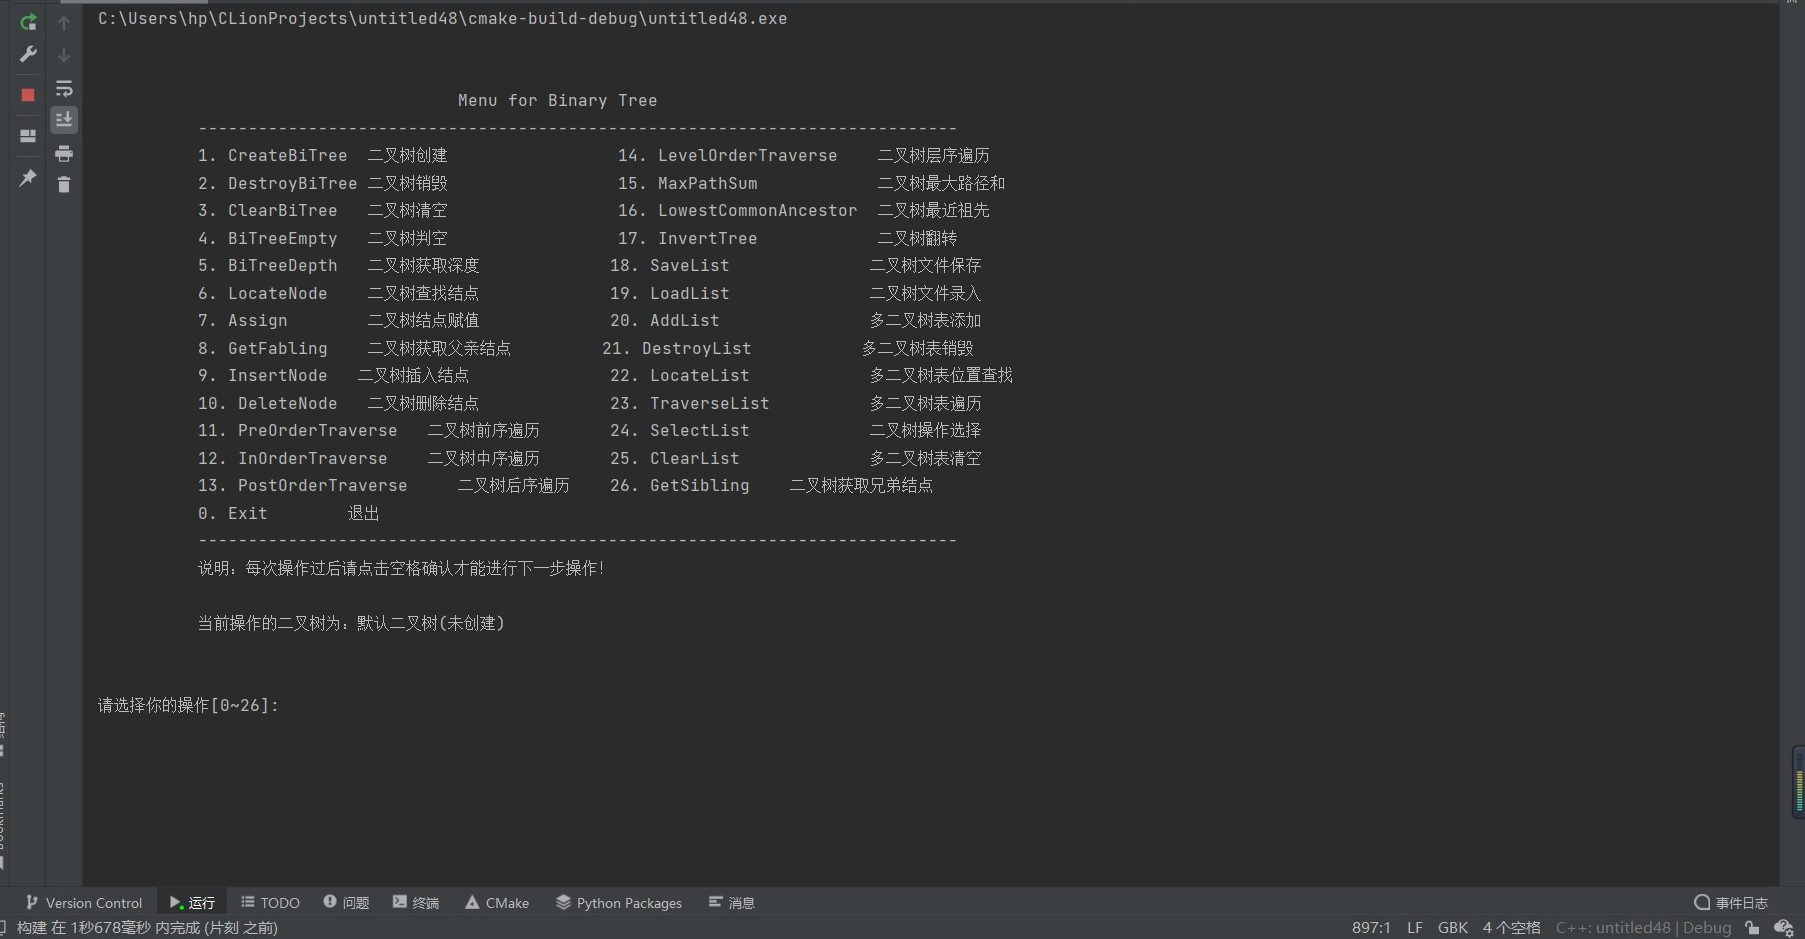
\includegraphics[width=0.8\textwidth]{images/二叉树菜单.jpg}
 	\caption{菜单}
 	\label{txlab}
 \end{figure}

测试集如下:

测试集1:1 a 2 b 0 null  0 null 3 c 4 d  0 null  0 null 5 e  0 null  0 null -1 null

测试集2:森林中创建两个二叉树

FirstTree:1 a 2 b 0 null  0 null 3 c 4 d  0 null  0 null 5 e  0 null  0 null -1 null

SecondTree:1 a 2 b 0 null    3 c 4 d  0 null  5 e  0 null 0 null  0 null   0 null -1 null

\setcounter{paragraph}{0}

\subsubsection{基本功能函数测试}

\paragraph{ 1.}.CreateBiTree测试

测试1:将使用测试集1,测试函数能否正确构造二叉树,通过先序遍历和中序遍历的方法来检验正确性;

测试2:将使用关键字重复的序列1(1 a 2 b 0 null 0 null 3 c 4 d 0 null  0 null 3 e 0 null 0 null -1 null),测试函数能否给出判断;

测试3:将输入根节点为空的序列(0 null -1 null),测试函数能否正确创建二叉树。

测试4在测试集1的基础上测试能否判断已有二叉树。

(注:为了排版方便,测试用例在上文中给出)

\vspace{0.5em}

\begin{tabular}{|c|l|p{6cm}|c|c|}
	\hline
	测试编号 & 测试输入 & 预期结果 & 实际运行结果 \\
	\hline
	1 & 1$\rightarrow$测试集1 & 二叉树创建成功!

先序遍历:1,a 2,b 3,c 4,d 5,e

中序遍历:2,b 1,a 4,d 3,c 5,e & 一致 \\
	\hline
	2 & 1$\rightarrow$序列1 & 关键字不唯一!创建失败! & 一致 \\
	\hline
	3 & 1$\rightarrow$序列2 & 二叉树创建成功! & 一致 \\
	\hline
	4 & 1$\rightarrow$测试集1 & 该二叉树已存在! & 一致 \\
	\hline
\end{tabular}

~\

 \begin{figure}[H]
 	\centering
 	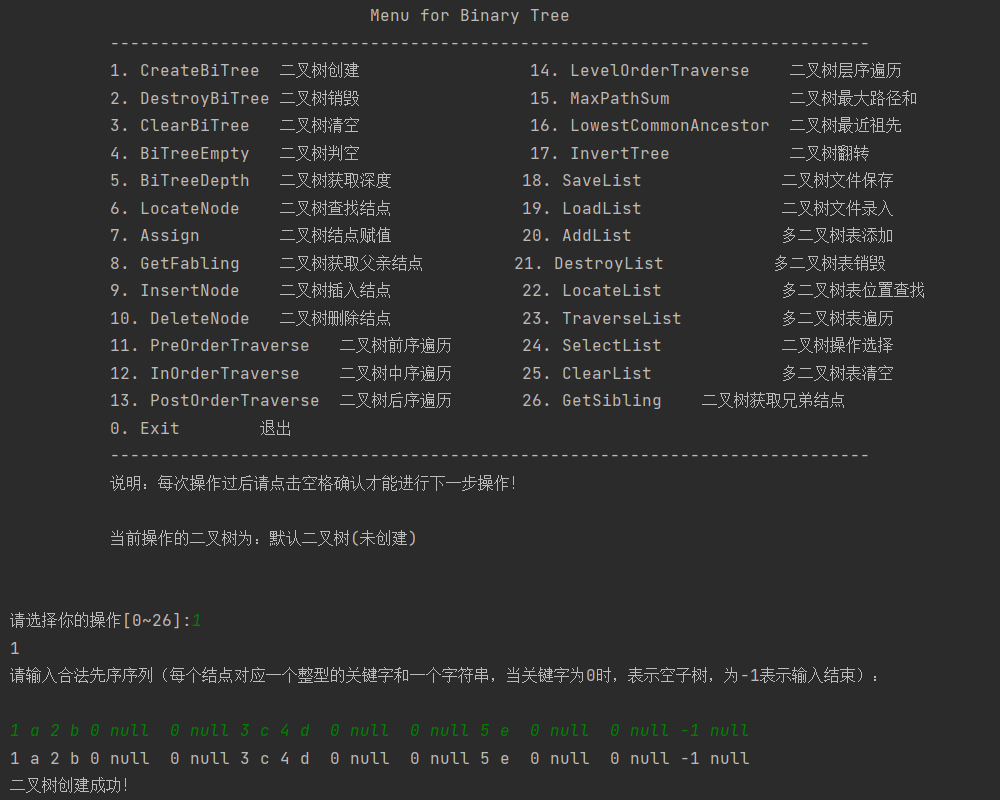
\includegraphics[width=0.6\textwidth]{images/二叉树测试1.png}
 	\caption{测试3运行结果}
 	\label{txlab}
 \end{figure}

\paragraph{ 2.}DestroyBiTree测试

测试1:将测试函数能否销毁不存在的二叉树;

测试2:在测试集1的情况下进行,测试函数能否销毁已存在的二叉树。

\vspace{0.5em}

\begin{tabular}{|c|l|c|c|c|}
	\hline
	测试编号 & 测试输入 & 预期结果 & 实际运行结果 \\
	\hline
	1 & 2 & 二叉树为空! & 一致 \\
	\hline
	2 & 1$\rightarrow$2 & 二叉树销毁成功! & 一致 \\
	\hline
\end{tabular}

~\

\begin{figure}[H]
 	\centering
 	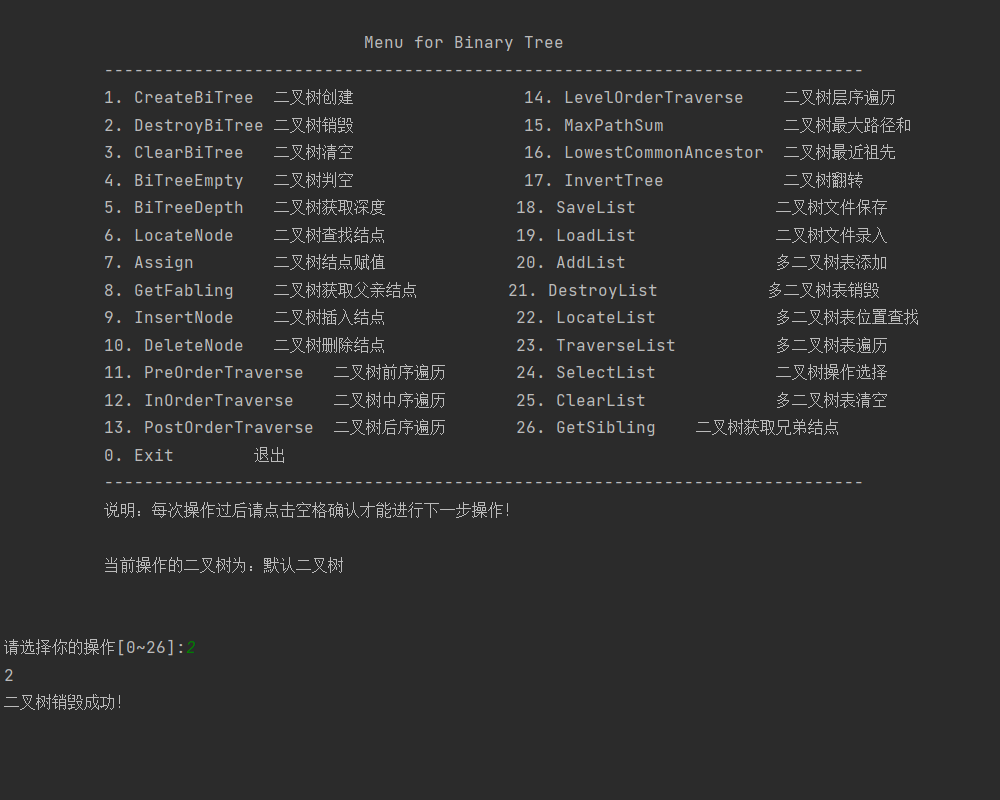
\includegraphics[width=0.6\textwidth]{images/二叉树测试2.png}
 	\caption{测试2运行结果}
 	\label{txlab}
 \end{figure}

\paragraph{ 3.}ClearBiTree测试

测试1:将测试函数能否清空不存在的二叉树;

测试2:在测试集1的情况下进行,测试函数能否清空已存在的二叉树。

\vspace{0.5em}

\begin{tabular}{|c|l|c|c|c|}
	\hline
	测试编号 & 测试输入 & 预期结果 & 实际运行结果 \\
	\hline
	1 & 3 & 二叉树为空! & 一致 \\
	\hline
	2 & 1$\rightarrow$3 & 二叉树清空成功! & 一致 \\
	\hline
\end{tabular}

~\

\begin{figure}[H]
 	\centering
 	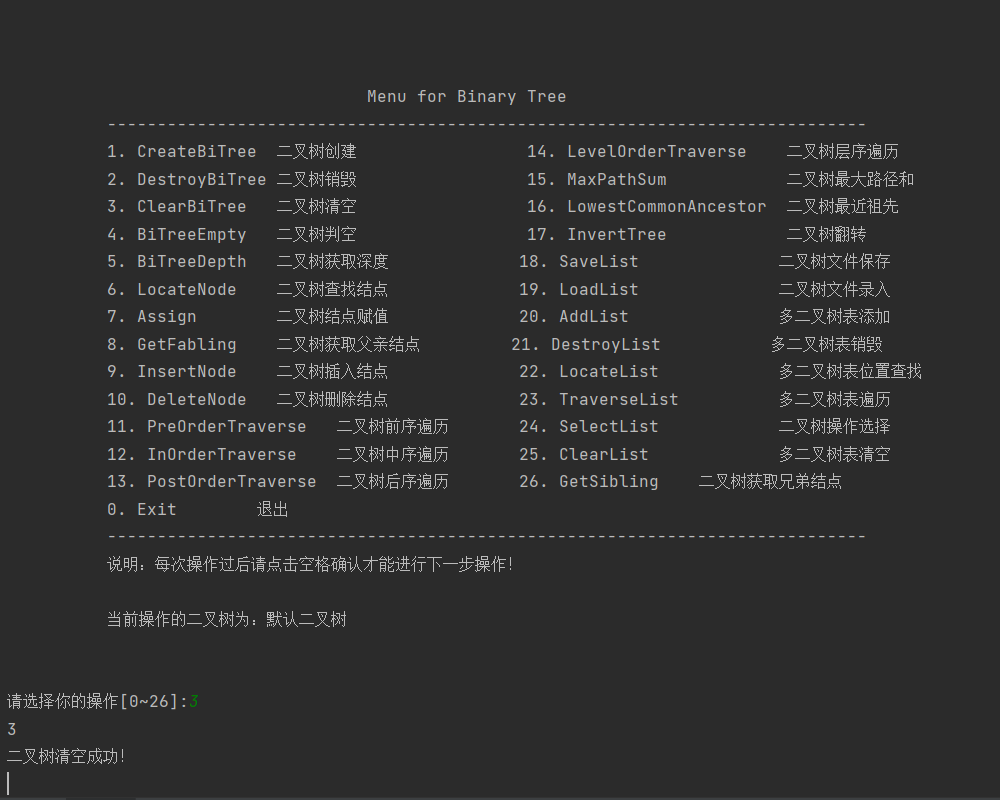
\includegraphics[width=0.6\textwidth]{images/二叉树测试3.png}
 	\caption{测试2运行结果}
 	\label{txlab}
 \end{figure}

\paragraph{ 4.}BiTreeEmpty测试

测试1:测试函数是否能对空二叉树进行判空;

测试2:在测试集1的基础上,测试函数是否能对非空二叉树进行判空。

\vspace{0.5em}

\begin{tabular}{|c|l|c|c|c|}
	\hline
	测试编号 & 测试输入 & 预期结果 & 实际运行结果 \\
	\hline
	1 & 4 & 二叉树为空! & 一致 \\
	\hline
	2 & 1$\rightarrow$4 & 二叉树不为空! & 一致 \\
	\hline
\end{tabular}

~\

\begin{figure}[H]
 	\centering
 	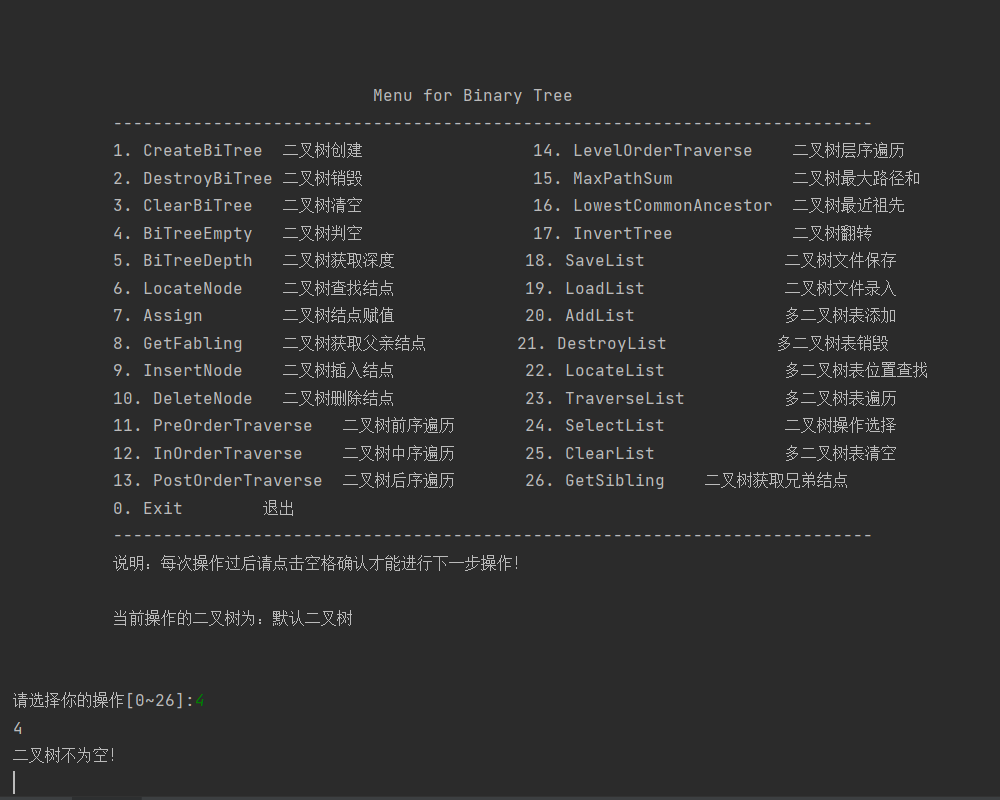
\includegraphics[width=0.6\textwidth]{images/二叉树测试4.png}
 	\caption{测试2运行结果}
 	\label{txlab}
 \end{figure}

\paragraph{ 5.}BiTreeDepth测试

测试1:测试函数能否对空二叉树求深度;

测试2:在测试集1的基础上,测试函数能否正确求得二叉树的深度。

\vspace{0.5em}

\begin{tabular}{|c|l|c|c|c|}
	\hline
	测试编号 & 测试输入 & 预期结果 & 实际运行结果 \\
	\hline
	1 & 5 & 二叉树为空! & 一致 \\
	\hline
	2 & 1$\rightarrow$5 & 该二叉树的深度为3! & 一致 \\
	\hline
\end{tabular}

~\

\begin{figure}[H]
 	\centering
 	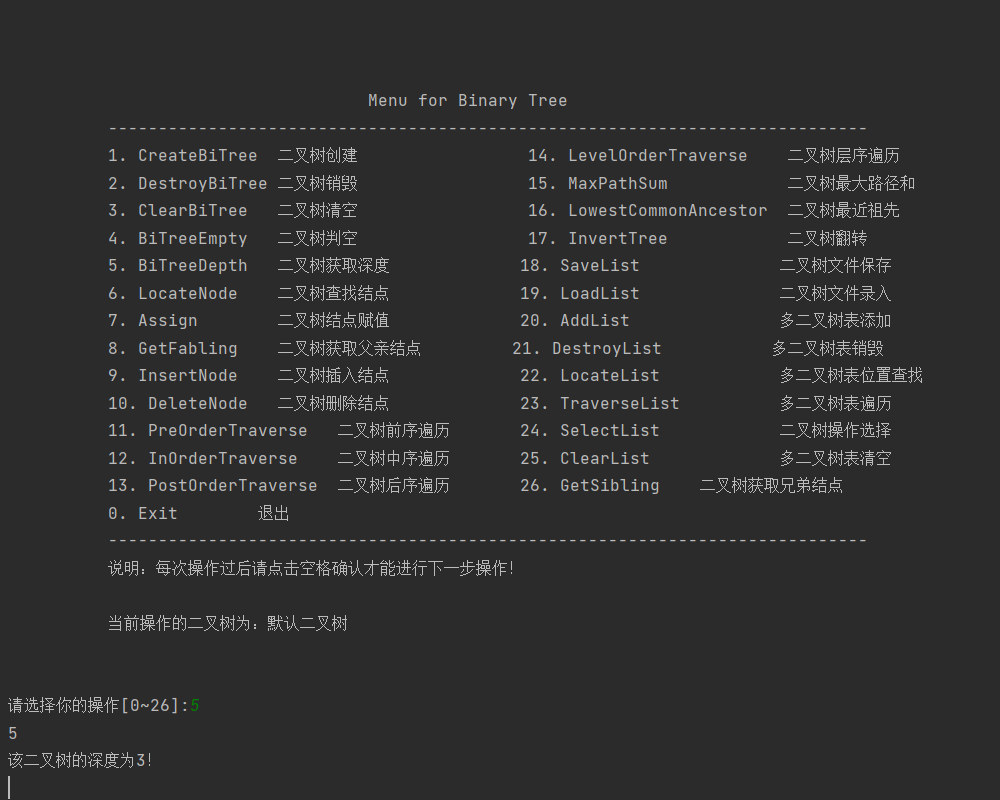
\includegraphics[width=0.6\textwidth]{images/二叉树测试5.png}
 	\caption{测试2运行结果}
 	\label{txlab}
 \end{figure}

\paragraph{ 6.}LocateNode测试

本函数的测试在测试集1的情况下进行。

测试1:将测试函数能否正确找到头结点并输出其值;

测试2:将测试函数能否正确找到一般结点并输出其值;

测试3:将测试函数能否正确判断结点关键字不在二叉树中。

\vspace{0.5em}

\begin{tabular}{|c|l|c|c|c|}
	\hline
	测试编号 & 测试输入 & 预期结果 & 实际运行结果 \\
	\hline
	1 & 6$\rightarrow$1 & 该节点存在!结点信息为:a & 一致 \\
	\hline
	2 & 6$\rightarrow$3 & 该节点存在!结点信息为:c & 一致 \\
	\hline
	3 & 6$\rightarrow$6 & 该节点不存在! & 一致 \\
	\hline
\end{tabular}

~\

\begin{figure}[H]
 	\centering
 	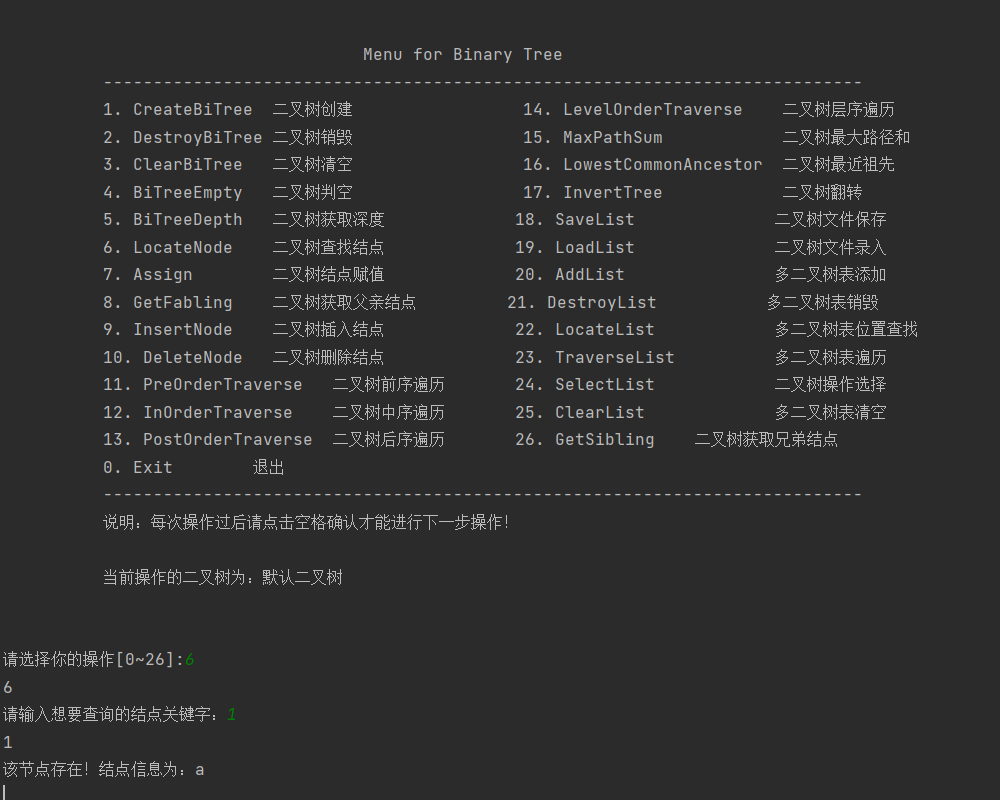
\includegraphics[width=0.6\textwidth]{images/二叉树测试6.png}
 	\caption{测试1运行结果}
 	\label{txlab}
 \end{figure}

\paragraph{ 7.}Assign测试

本函数的测试在测试集1的情况下进行。

输入要求:先输入想要修改的结点关键字,再输入修改后的值,同时测试为顺序进行。

测试1:将测试在修改结点值时,函数能否输出正确结果(通过先序遍历结果判断);

测试2:将测试在修改结点值,但修改后关键字重复的情况下,函数能否给出判断;

测试3:将测试所修改结点不在二叉树中的情况下,函数能否给出判断。

\vspace{0.5em}

\begin{tabular}{|c|l|p{6cm}|c|}
	\hline
	测试编号 & 测试输入 & 预期结果 & 实际运行结果 \\
	\hline
	1 & 7$\rightarrow$5$\rightarrow$6 f & 结点赋值成功!

先序遍历:1,a 2,b 3,c 4,d 6,f & 一致 \\
	\hline
	2 & 7$\rightarrow$1$\rightarrow$2 g & 结点复制失败(请检查该关键字是否存在或者赋值关键字是否重复) & 一致 \\
	\hline
	3 & 7$\rightarrow$7$\rightarrow$8 h & 结点复制失败(请检查该关键字是否存在或者赋值关键字是否重复) & 一致 \\
	\hline
\end{tabular}

~\

\begin{figure}[H]
 	\centering
 	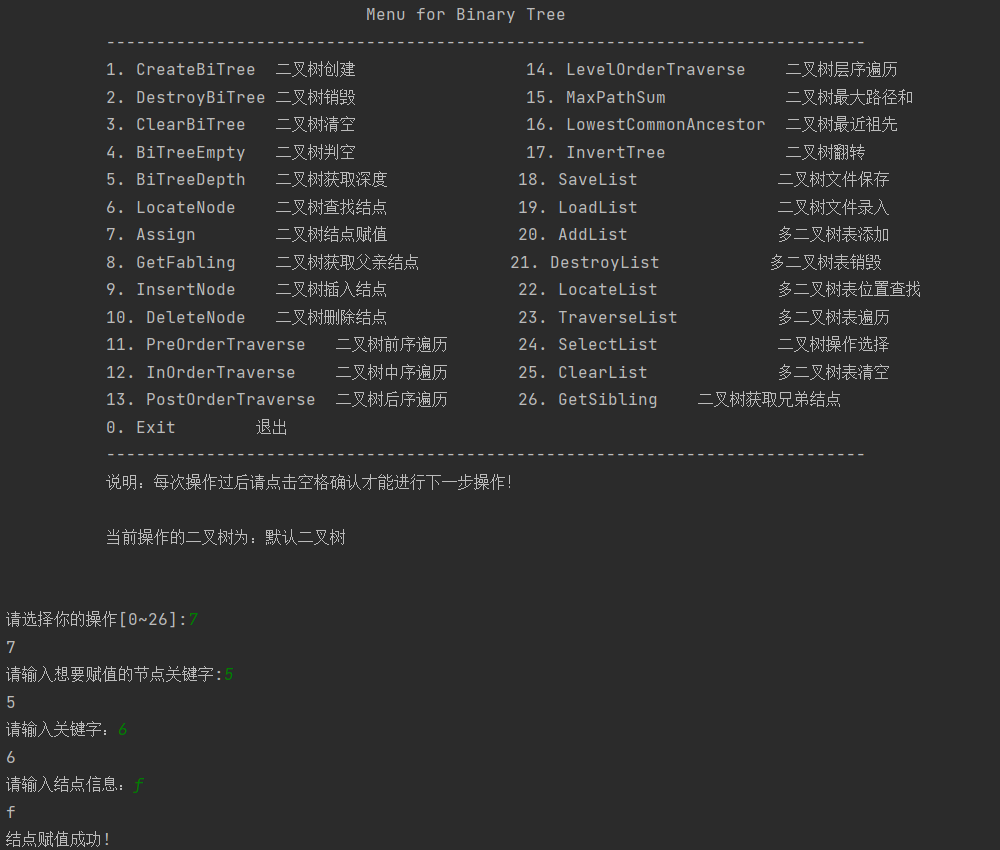
\includegraphics[width=0.6\textwidth]{images/二叉树测试7.png}
 	\caption{测试1运行结果}
 	\label{txlab}
 \end{figure}

\paragraph{ 8.}GetSibling测试

本函数的测试在测试集1的情况下进行。

测试1,2:将输入一组互为兄弟的结点,测试函数能否输出正确结果;

测试3:将输入没有兄弟结点的结点,测试函数能否输出正确结果;

测试4:将输入一个不在二叉树中的结点,测试函数能否给出判断。

\vspace{0.5em}

\begin{tabular}{|c|l|p{7cm}|c|}
	\hline
	测试编号 & 测试输入 & 预期结果 & 实际运行结果 \\
	\hline
	1 & 8$\rightarrow$5 & 该元素兄弟结点获取成功!

该结点的兄弟结点关键字为 4 结点信息为: d & 一致 \\
	\hline
	2 & 8$\rightarrow$4 & 该元素兄弟结点获取成功!

该结点的兄弟结点关键字为 5 结点信息为: e & 一致 \\
	\hline
	3 & 8$\rightarrow$1 & 该结点不存在或不存在兄弟结点! & 一致 \\
	\hline
	4 & 8$\rightarrow$6 & 该结点不存在或不存在兄弟结点! & 一致 \\
	\hline
\end{tabular}

~\

\begin{figure}[H]
 	\centering
 	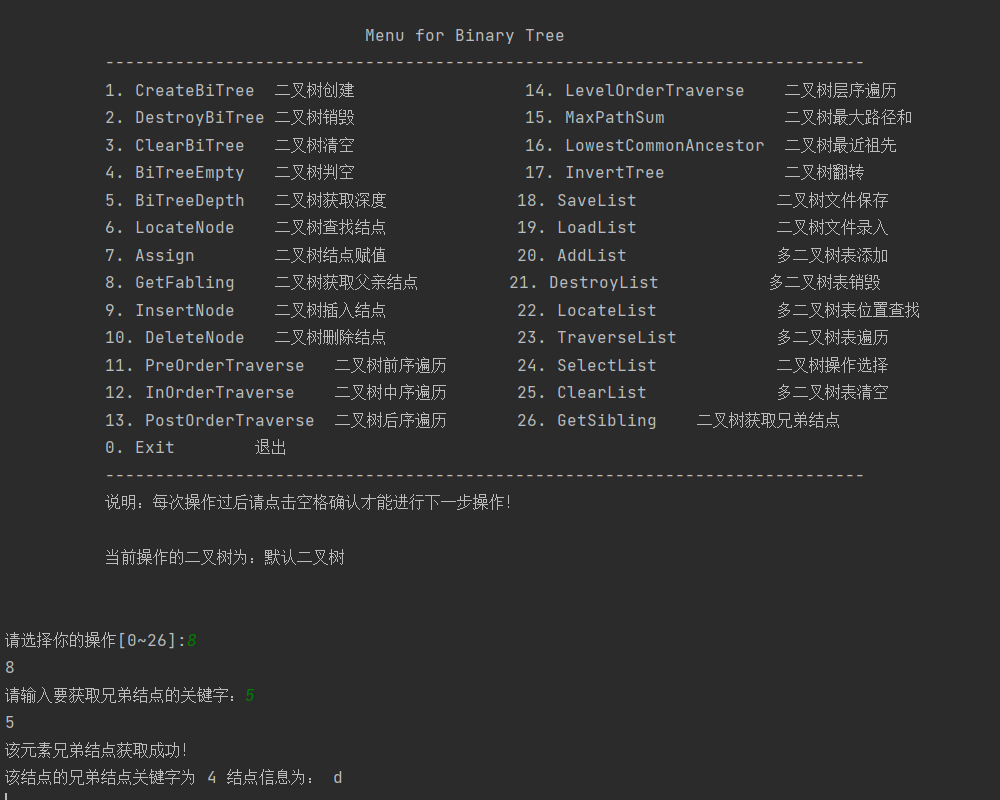
\includegraphics[width=0.6\textwidth]{images/二叉树测试8.png}
 	\caption{测试1运行结果}
 	\label{txlab}
 \end{figure}

\paragraph{ 9.}InsertNode测试

输入要求:首先输入结点父亲的关键字,再输入插入要求(左孩子(0)/右孩子(1)/根节点(-1),如插入结点作为根节点,则无需考虑结点父亲的值),最后输入插入结点的值。

测试1:在测试集1的情况下进行,将新插入结点(6 f)作为根节点(-1),测试函数能否输出正确结果,通过前序遍历检验正确性;

测试2:在测试集1的情况下进行,在根节点(1 a)的左孩子插入结点(6 f),测试函数能否输出正确结果,通过前序遍历检验正确性;

测试3:在测试集1的情况下进行,在根节点(1 a)的右孩子插入结点(6 f),测试函数能否输出正确结果,通过前序遍历检验正确性;

测试4:在测试集1的情况下进行,尝试在根节点处插入一个关键字重复的结点(2 b),测试函数能否给出正确判断;

测试5:在测试集1的情况下进行,尝试插入一个结点(6 f),测试当输入的父亲结点(6)不存在于二叉树中时,函数能否给出正确的判断。

\vspace{0.5em}

\begin{tabular}{|c|l|p{6cm}|c|}
	\hline
	测试编号 & 测试输入 & 预期结果 & 实际运行结果 \\
	\hline
	1 & 9$\rightarrow$1$\rightarrow$6 f -1 & 结点插入成功!

前序遍历: 6,f 1,a 2,b 3,c 4,d 5,e & 一致 \\
	\hline
	2 & 9$\rightarrow$1$\rightarrow$6 f 0 & 结点插入成功!

前序遍历:  1,a 6,f 2,b 3,c 4,d 5,e & 一致 \\
	\hline
	3 & 9$\rightarrow$1$\rightarrow$2 b 1 & 结点插入失败(请检查该关键字是否存在或者插入关键字是否重复)! & 一致 \\
	\hline
	3 & 9$\rightarrow$6$\rightarrow$6 f 1 & 结点插入失败(请检查该关键字是否存在或者插入关键字是否重复)! & 一致 \\
	\hline
\end{tabular}

~\

\begin{figure}[H]
 	\centering
 	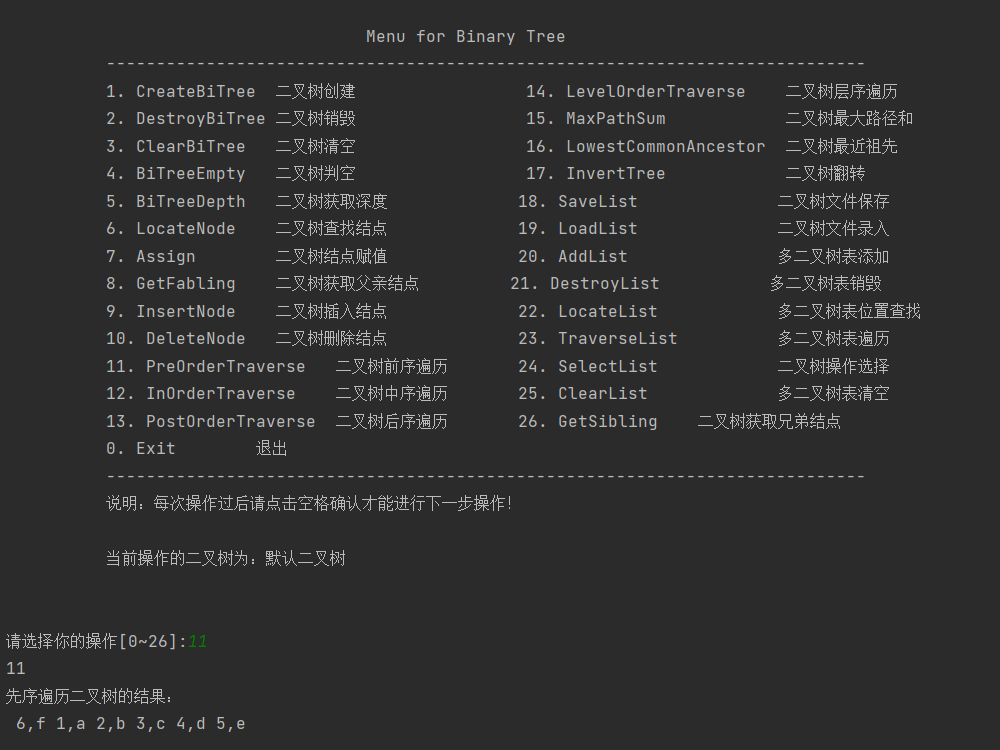
\includegraphics[width=0.6\textwidth]{images/二叉树测试9.png}
 	\caption{测试1运行结果}
 	\label{txlab}
 \end{figure}

\paragraph{10.}DeleteNode测试

测试1:在测试集1的情况下进行,测试函数能否正确删除度为2的根结点,通过层序遍历的方式来检验正确性;

测试2:在测试1的基础上进行,测试函数能否正确删除度为0的叶子结点,通过层序遍历的方式来检验正确性;

测试3:在测试2的基础上进行,测试函数能否正确删除度为1的结点,通过层序遍历的方式来检验正确性。

\vspace{0.5em}

\begin{tabular}{|c|l|l|c|}
	\hline
	测试编号 & 测试输入 & 预期结果 & 实际运行结果 \\
	\hline
	1 & 10$\rightarrow$3& 结点删除成功!

层序遍历: 1,a 2,b 4,d 5,e & 一致 \\
	\hline
	2 & 10$\rightarrow$2& 结点删除成功!

层序遍历: 1,a 4,d 5,e & 一致 \\
	\hline
	3 & 10$\rightarrow$4 & 结点删除成功!

层序遍历:1,a 5,e & 一致 \\
	\hline
\end{tabular}

~\

\begin{figure}[H]
 	\centering
 	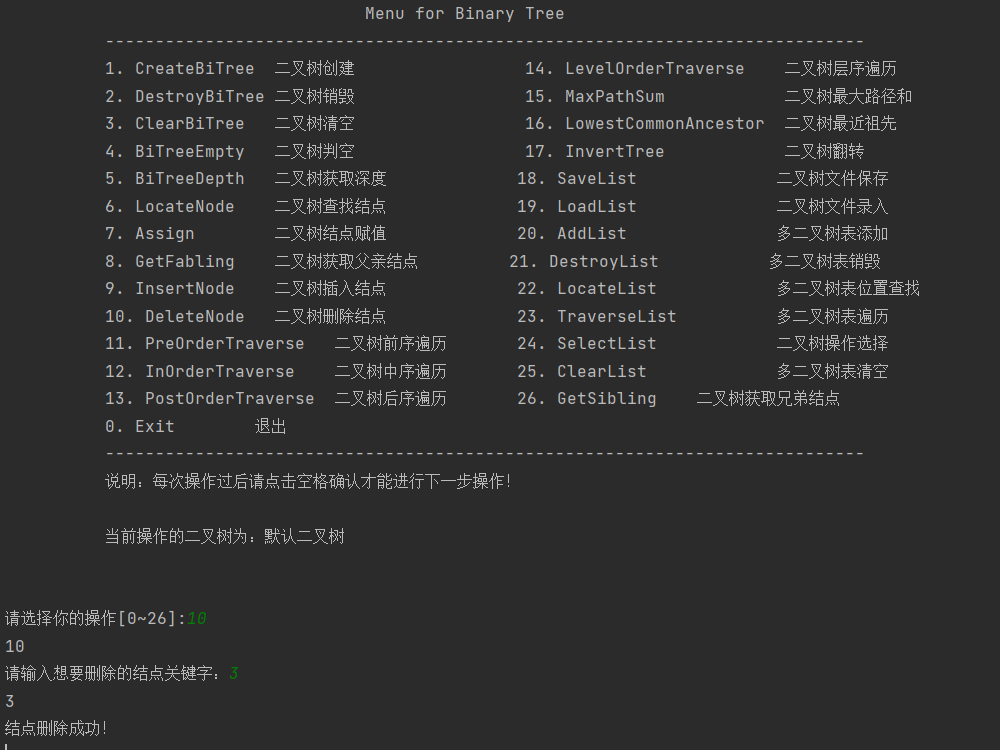
\includegraphics[width=0.6\textwidth]{images/二叉树测试10.png}
 	\caption{测试1运行结果}
 	\label{txlab}
 \end{figure}

\paragraph{11.}PreOrderTraverse测试

测试1:将测试函数是否能对空树做出判断;

测试2:在测试集1的情况下进行,测试函数能否输出正确结果。

\vspace{0.5em}

\begin{tabular}{|c|p{2.7cm}|p{4.5cm}|c|}
	\hline
	测试编号 & 测试输入 & 预期结果 & 实际运行结果 \\
	\hline
	1 & 11 & 二叉树为空! & 一致 \\
	\hline
	2 & 11 & 先序遍历二叉树的结果:
 
1,a 2,b 3,c 4,d 5,e & 一致 \\
	\hline
\end{tabular}

~\

\begin{figure}[H]
 	\centering
 	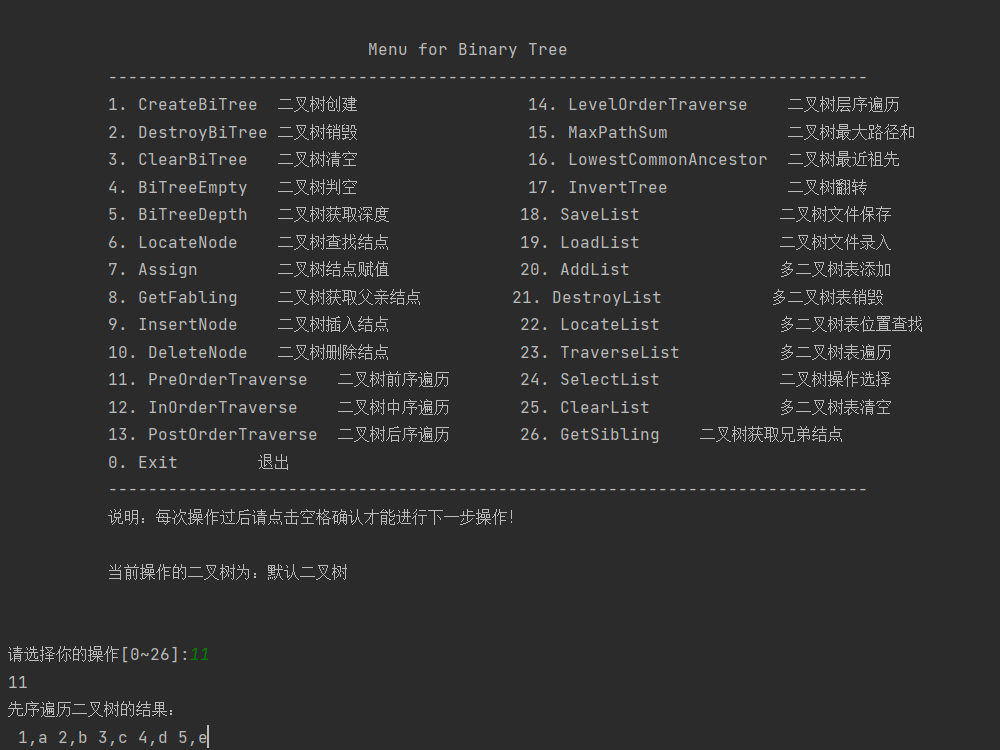
\includegraphics[width=0.6\textwidth]{images/二叉树测试11.png}
 	\caption{测试2运行结果}
 	\label{txlab}
 \end{figure}

\paragraph{12.}InOrderTraverse测试

测试1:将测试函数是否能对空树做出判断;

测试2:在测试集1的情况下进行,测试函数能否输出正确结果。

\vspace{0.5em}

\begin{tabular}{|c|p{2.7cm}|p{4.5cm}|c|}
	\hline
	测试编号 & 测试输入 & 预期结果 & 实际运行结果 \\
	\hline
	1 & 12 & 二叉树为空! & 一致 \\
	\hline
	2 & 12 & 中序遍历二叉树的结果:
 
2,b 1,a 4,d 3,c 5,e & 一致 \\
	\hline
\end{tabular}

~\

\begin{figure}[H]
 	\centering
 	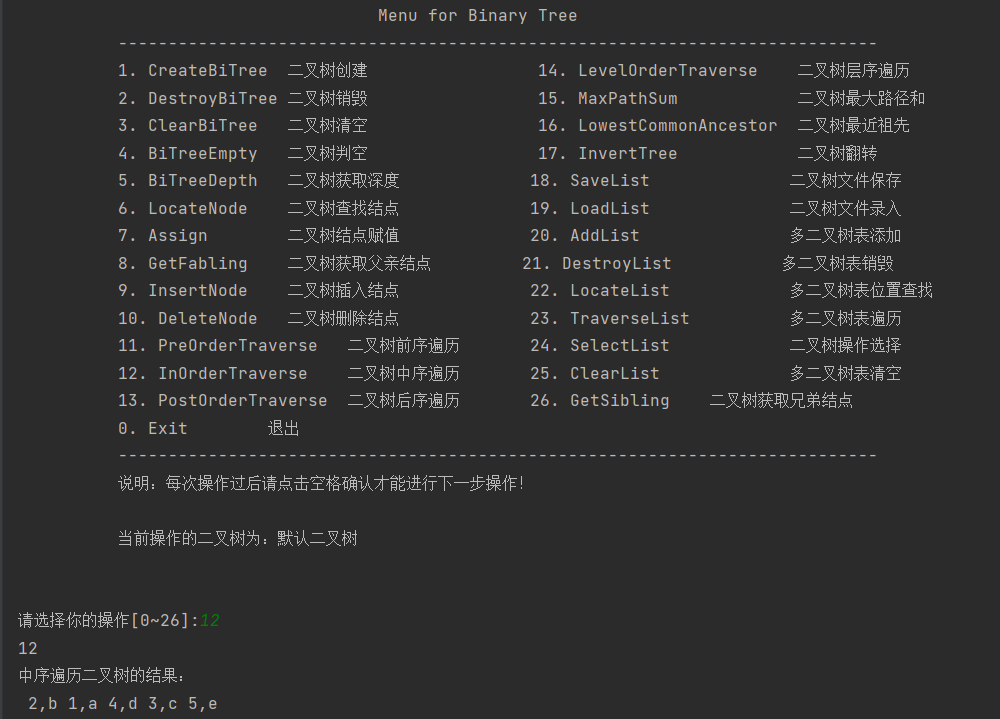
\includegraphics[width=0.6\textwidth]{images/二叉树测试12.png}
 	\caption{测试2运行结果}
 	\label{txlab}
 \end{figure}

\paragraph{13.}PostOrderTraverse测试

测试1:将测试函数是否能对空树做出判断;

测试2:在测试集1的情况下进行,测试函数能否输出正确结果。

\vspace{0.5em}

\begin{tabular}{|c|p{2.7cm}|p{4.5cm}|c|}
	\hline
	测试编号 & 测试输入 & 预期结果 & 实际运行结果 \\
	\hline
	1 & 13 & 二叉树为空! & 一致 \\
	\hline
	2 & 13 & 后序遍历二叉树的结果:
 
2,b 4,d 5,e 3,c 1,a & 一致 \\
	\hline
\end{tabular}

~\

\begin{figure}[H]
 	\centering
 	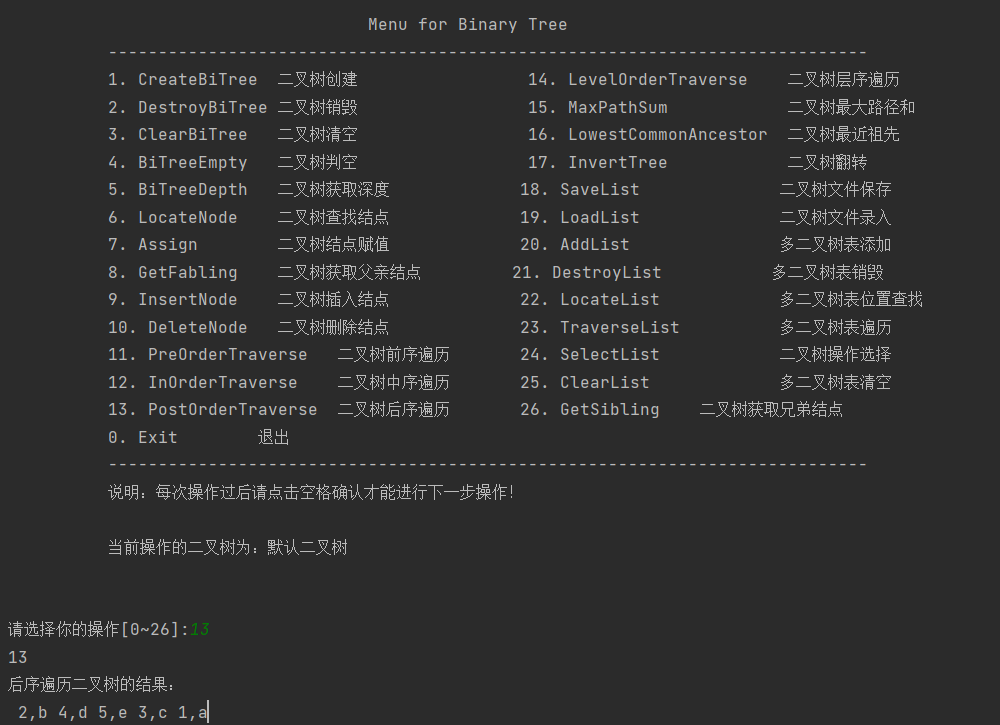
\includegraphics[width=0.6\textwidth]{images/二叉树测试13.png}
 	\caption{测试2运行结果}
 	\label{txlab}
 \end{figure}

\paragraph{14.}LevelOrderTraverse测试

测试1:将测试函数是否能对空树做出判断;

测试2:在测试集1的情况下进行,测试函数能否输出正确结果。

\vspace{0.5em}

\begin{tabular}{|c|p{2.7cm}|p{4.5cm}|c|}
	\hline
	测试编号 & 测试输入 & 预期结果 & 实际运行结果 \\
	\hline
	1 & 14 & 二叉树为空! & 一致 \\
	\hline
	2 & 14 & 层序遍历二叉树的结果:

 1,a 2,b 3,c 4,d 5,e & 一致 \\
	\hline
\end{tabular}

~\

\begin{figure}[H]
 	\centering
 	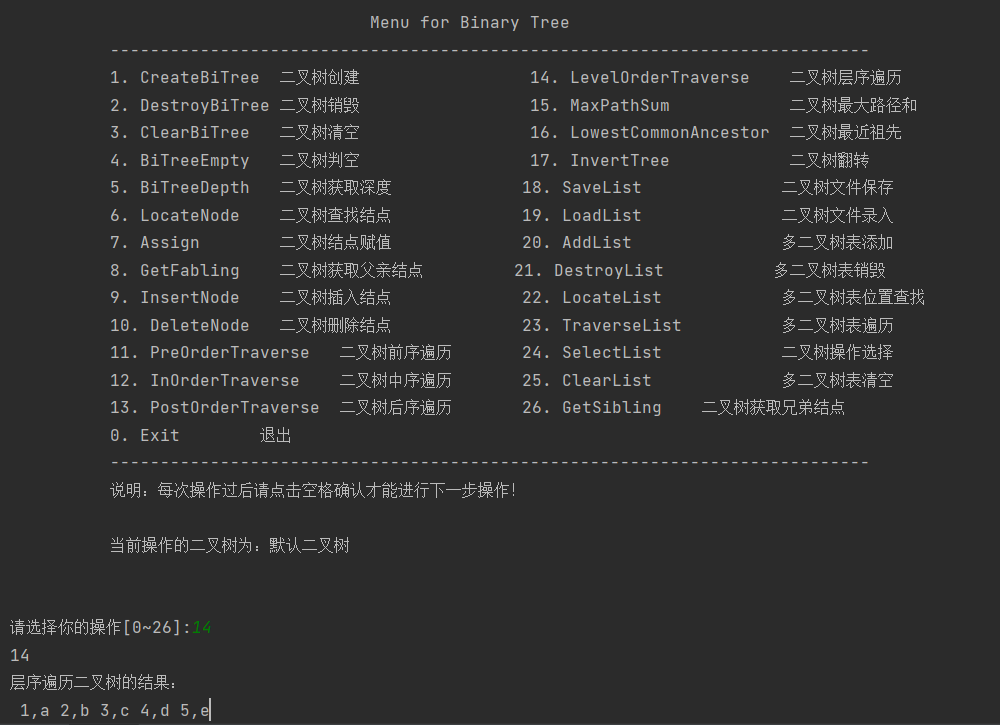
\includegraphics[width=0.6\textwidth]{images/二叉树测试14.png}
 	\caption{测试2运行结果}
 	\label{txlab}
 \end{figure}

\subsubsection{附加功能测试}

\paragraph{15.}MaxPathSum测试
	
测试1:在二叉树为空的情况下进行,测试函数能否给出正确判断;

测试2:在测试集1的情况下进行,测试函数能否正常返回最大路径和。

\vspace{0.5em}

\begin{tabular}{|c|p{2.7cm}|p{6cm}|c|}
	\hline
	测试编号 & 测试输入 & 预期结果 & 实际运行结果 \\
	\hline
	1 & 15 & 二叉树为空! & 一致 \\
	\hline
	2 & 15 & 根节点到叶子结点的最大路径和为:9 & 一致 \\
	\hline
\end{tabular}

~\

\paragraph{16.}LowestCommonAncestor测试
	
测试1:在二叉树为空的情况下进行,测试函数能否给出正确判断;

测试2:在测试集1的情况下进行,两结点均存在测试能否给出根结点;

测试3:在测试集1的情况下进行,测试第一个结点不存在时能否给出正确的判断;

测试4:在测试集1的情况下进行,测试第二个结点不存在时能否给出正确的判断。

\vspace{0.5em}

\begin{tabular}{|c|p{2.7cm}|p{6cm}|c|}
	\hline
	测试编号 & 测试输入 & 预期结果 & 实际运行结果 \\
	\hline
	1 & 16 & 二叉树为空! & 一致 \\
	\hline
	2 & 16$\rightarrow$2 4 & 两结点最近公共祖先的关键字为:1,结点信息为:a & 一致 \\
	\hline
	3 & 16$\rightarrow$6 4 & 第一个结点不存在!& 一致 \\
	\hline
	4 & 16$\rightarrow$2 6 & 第二个结点不存在! & 一致 \\
	\hline
\end{tabular}

~\

\paragraph{17.}InvertTree测试

测试1:在二叉树为空的情况下进行,测试函数能否给出正确判断;

测试2:在测试集1的情况下,测试函数能否正确反转二叉树,通过层序遍历测试函数实现正确性。

\vspace{0.5em}

\begin{tabular}{|c|p{2.7cm}|p{6cm}|c|}
	\hline
	测试编号 & 测试输入 & 预期结果 & 实际运行结果 \\
	\hline
	1 & 17 & 二叉树为空! & 一致 \\
	\hline
	2 & 17$\rightarrow$14 & 二叉树翻转成功!

层序遍历二叉树的结果:1,a 3,c 2,b 5,e 4,d & 一致 \\
	\hline
\end{tabular}

~\

\paragraph{18.}SaveList测试

测试1:在测试集1的情况下进行,测试函数能否正常进行写文件操作;

测试2:在文件已经有内容时,测试函数是否能够判断文件不能覆盖;

测试3:在二叉树为空的情况下进行,测试函数能否给出正确判断。

\vspace{0.5em}

\begin{tabular}{|c|p{2.7cm}|c|c|}
	\hline
	测试编号 & 测试输入 & 预期结果 & 实际运行结果 \\
	\hline
	1 & 18$\rightarrow$1.txt & 文件保存成功! & 一致 \\
	\hline
	2 & 18$\rightarrow$1.txt & 该文件已有内容,不能读入! & 一致 \\
	\hline
	3 & 2$\rightarrow$18$\rightarrow$1.txt & 二叉树不存在!文件保存失败! & 一致 \\
	\hline
\end{tabular}

~\

\paragraph{19.}LoadList测试
	
本函数的测试都在文件1中已存有测试集1的情况下进行。

测试1:在二叉树不存在的情况下进行,测试函数能否正确进行读文件操作,采用遍历二叉树的方式检验正确性。

测试2:在线性表存在的情况下进行,测试函数能否给出正确判断。

\vspace{0.5em}

\begin{tabular}{|c|p{2.7cm}|c|c|}
	\hline
	测试编号 & 测试输入 & 预期结果 & 实际运行结果 \\
	\hline
	1 & 2$\rightarrow$19$\rightarrow$1.txt & 文件录入成功! & 一致 \\
	\hline
	2 & 19$\rightarrow$1.txt & 二叉树存在!文件录入失败 & 一致 \\
	\hline
\end{tabular}

~\

\paragraph{20.}AddList测试

测试1:将测试函数能否正确添加二叉树;

测试2:在测试1的基础上进行,当二叉树名称重复时,测试函数能否给出正确的判断。

测试3:构建测试集3,测试二叉树能否正确添加,通过遍历森林检验正确性。

\vspace{0.5em}

\begin{tabular}{|c|p{2.7cm}|c|c|}
	\hline
	测试编号 & 测试输入 & 预期结果 & 实际运行结果 \\
	\hline
	1 & 20$\rightarrow$FirstTree & FirstTree已成功添加! & 一致 \\
	\hline
	2 & 20$\rightarrow$FirstTree & 该名称的线性表已经存在! & 一致 \\
	\hline
	3 & 213& FirstTree SecondTree & 一致 \\
	\hline
\end{tabular}

~\

\paragraph{21.}DestoryList测试

本函数的测试在测试集2的基础上进行。

测试1:将测试函数能否正确销毁二叉树,采用遍历森林的方式判断正确性;

测试2:在测试集2的情况下进行,尝试销毁一个不在集合中的二叉树,测试函数能否给出正确判断。

\vspace{0.5em}

\begin{tabular}{|c|p{2.7cm}|c|c|}
	\hline
	测试编号 & 测试输入 & 预期结果 & 实际运行结果 \\
	\hline
	1 & 21$\rightarrow$FirstTree & FirstTree已成功销毁! & 一致 \\
	\hline
	2 & 21$\rightarrow$ThirdTree & 二叉树不存在! & 一致 \\
	\hline
\end{tabular}

~\

\paragraph{22.}LocateList测试
	
本函数的测试在测试集2的基础上进行。

测试1:将测试函数能否正确定位二叉树;

测试2:将尝试查找一个不在集合中的二叉树,测试函数能否给出正确判断。

\vspace{0.5em}

\begin{tabular}{|c|p{2.7cm}|c|c|}
	\hline
	测试编号 & 测试输入 & 预期结果 & 实际运行结果 \\
	\hline
	1 & 22$\rightarrow$FirstTree & 该二叉树的逻辑索引为:1 & 一致 \\
	\hline
	2 & 22$\rightarrow$ThirdTree & 二叉树查找失败! & 一致 \\
	\hline
\end{tabular}

~\

\paragraph{23.}TraverseList测试
	
测试1:在测试集3的基础上进行,测试函数能否正确遍历各个线性表;

测试2:在空集合的基础上进行,测试函数能否给出正确判断。

\vspace{0.5em}

\begin{tabular}{|c|p{2.7cm}|c|c|}
	\hline
	测试编号 & 测试输入 & 预期结果 & 实际运行结果 \\
	\hline
	1 & (测试集2)23 & FirstList SecondList & 一致 \\
	\hline
	2 & 23 & 多二叉树表为空! & 一致 \\
	\hline
\end{tabular}

~\

\paragraph{24.}SelectList测试
	
输入要求:输入线性表集合中线性表对应的逻辑索引。
	
测试1,2:在测试集3的情况下进行,测试函数能否正确判断非法的位序;

测试3:在测试集3的情况下进行,测试函数能否正确地实现选取线性表操作。

\vspace{0.5em}

\begin{tabular}{|c|p{2.7cm}|c|c|}
	\hline
	测试编号 & 测试输入 & 预期结果 & 实际运行结果 \\
	\hline
	1 & 24$\rightarrow$0 & 二叉树选取失败! & 一致 \\
	\hline
	1 & 24$\rightarrow$3 & 二叉树选取失败! & 一致 \\
	\hline
	2 & 24$\rightarrow$1 & 二叉树已选取成功! & 一致 \\
	\hline
\end{tabular}

~\

测试小结

24个函数基本符合了测试要求,在正常和异常用例的条件下均可以正常运行。需要注意的是,在对某些函数进行测试时,出于篇幅限制,没有测试二叉树不存在的情况,同时对于附加功能函数没有具体给测试后的控制台界面。(25,26函数属于辅助函数,对于测试不做要求。)

\subsection{实验小结}

这次实验使用链式存储结构实现二叉树,让我更加清楚了二叉树的物理结构、数据结构类型、基本操作及实现。认识到二叉树的存储结构与线性存储结构的不同。这次实验中使用顺序表来管理多树(森林),提高了本次实验的程序的功能性。

在本次实验过程中,多个函数使用递归调用自身的形式编写函数,同时通过设置全局变量的方式解决递归过程中变量的初始化和迭代问题。

除此以外,在用非递归方式实现遍历时,使用了栈的存储结构和相应操作,在实现层序遍历时,使用了队列的存储结构和相应操作。通过不同数据结构的运用,使得问题的解决更加便利。

同时,基于二叉链表的二叉树的实验的难度较前两次都有所提升,极大地提升了我的编程水平。

本次实验使我加深了对二叉树的概念、基本运算的理解,掌握了二叉树的基本运算的实现。熟练了二叉树的逻辑结构和物理结构的关系。在今后的学习过程当中应该更多地从数据结构的角度去分析如何进行数据的存储、读取和处理,以达到更简便地解决实际问题的目的。


\newpage

\section{课程的收获和建议}

通过本学期的数据结构实验课,我收获了很多知识,非常感谢老师和助教的帮助,同时包括我自己的努力,让我在数据结构方面收获很多,编程能力和思维能力有了很大的提高。

\subsection{基于顺序存储结构的线性表实现}

通过实验达到:(1)加深对线性表的概念、基本运算的理解;(2)熟练掌握线性表的逻辑结构与物理结构的关系;(3)物理结构采用顺序表,熟练掌握顺序表基本运算的实现。在实验过程中,对于线性表的本质有了更加深入的思考与理解,提升了思维能力。

\subsection{基于链式存储结构的线性表实现}

通过实验达到:(1)加深对线性表的概念、基本运算的理解;(2)熟练掌握线性表的逻辑结构与物理结构的关系;(3)物理结构采用单链表,熟练掌握线性表的基本运算的实现。在实验过程中,清晰了顺序存储结构和单链表存储结构之间的区别与联系,对于线性表有了深刻的体会,同时能够灵活应用。

\subsection{基于二叉链表的二叉树实现}

通过实验达到:(1)加深对二叉树的概念、基本运算的理解;(2)熟练掌握二叉树的逻辑结构与物理结构的关系;(3)以二叉链表作为物理结构,熟练掌握二叉树基本运算的实现。在实验过程中,对于二叉树特殊的存储结构能够很好地应用,同时对于递归操作有了更加深刻的理解。

\subsection{基于邻接表的图实现}

通过实验达到:(1)加深对图的概念、基本运算的理解;(2)熟练掌握图的逻辑结构与物理结构的关系;(3)以邻接表作为物理结构,熟练掌握图基本运算的实现。在实验过程中,学会使用图的邻接表创建无向图,同时由于图的复杂性,对于心理素质的锻炼起到了很大的效果。

\addcontentsline{toc}{section}{参考文献}
\nocite{*} %% 作用是不对文献进行引用,但可以生成文献列表
\bibliographystyle{HustGraduPaper}
\begin{thebibliography}{}
\bibitem[]{1}严蔚敏等.数据结构(C语言版).清华大学出版社
\bibitem[] {2}Larry Nyhoff. ADTs, Data Structures, and Problem Solving with C++.  Second Edition,Calvin College,2005
\bibitem[] {3}殷立峰. Qt C++跨平台图形界面程序设计基础. 清华大学出版社,2014:192~197
\bibitem[] {4}严蔚敏等.数据结构题集(C语言版).清华大学出版社
\end{thebibliography}

\section{附录A 基于顺序存储结构线性表实现的源程序}

\begin{lstlisting}[language=c]
#include <stdio.h>
#include <stdlib.h>
#include <string.h>
#include <windows.h>

#define TRUE 1
#define FALSE 0
#define OK 1
#define ERROR 0
#define INFEASIBLE -1
#define OVERFLOW -2
typedef int status;
typedef int ElemType; //数据元素类型定义
#define LIST_INIT_SIZE 100
#define LISTINCREMENT  10
#define MAXlength 10
typedef struct{  //顺序表(顺序结构)的定义
    ElemType * elem;
    int length;
    int listsize;
}SqList;
SqList L;

typedef struct{  //线性表的集合类型定义
    struct { char name[30];
        SqList L;
    } elem[11];
    int length;
}LISTS;
LISTS Lists;      //线性表集合的定义Lists

status InitList(SqList& L)
// 线性表L不存在,构造一个空的线性表,返回OK,否则返回INFEASIBLE。
{
    if(L.elem) return INFEASIBLE;
    L.elem = (ElemType *)malloc(LIST_INIT_SIZE * sizeof(ElemType));
    if(!L.elem)
        exit(OVERFLOW);
    L.length = 0;
    L.listsize = LIST_INIT_SIZE;
    return OK;

}

status DestroyList(SqList& L)
// 如果线性表L存在,销毁线性表L,释放数据元素的空间,返回OK,否则返回INFEASIBLE。
{
    if(!L.elem) return INFEASIBLE;
    free(L.elem);
    L.elem = NULL;
    return OK;

}

status ClearList(SqList& L)
// 如果线性表L存在,删除线性表L中的所有元素,返回OK,否则返回INFEASIBLE。
{
    if(!L.elem) return INFEASIBLE;
    L.length = 0;
    return OK;

}

status ListEmpty(SqList L)
// 如果线性表L存在,判断线性表L是否为空,空就返回TRUE,否则返回FALSE;如果线性表L不存在,返回INFEASIBLE。
{
    if(!L.elem) return INFEASIBLE;
    if(!L.length) return TRUE;
    else return FALSE;

}

status ListLength(SqList L)
// 如果线性表L存在,返回线性表L的长度,否则返回INFEASIBLE。
{
    if(!L.elem) return INFEASIBLE;
    return L.length;
}

status GetElem(SqList L,int i,ElemType &e)
// 如果线性表L存在,获取线性表L的第i个元素,保存在e中,返回OK;如果i不合法,返回ERROR;如果线性表L不存在,返回INFEASIBLE。
{
    if(!L.elem) return INFEASIBLE;
    if(i < 1 || i > L.length) return ERROR;
    e = L.elem[i - 1];
    return OK;

}

int compare(SqList L, int i, ElemType e){
	if(L.elem[i] == e) return 1;
	return 0;
}

int LocateElem(SqList L,ElemType e, int (*compare)(SqList, int, ElemType))
// 如果线性表L存在,查找元素e在线性表L中的位置序号并返回该序号;如果e不存在,返回0;当线性表L不存在时,返回INFEASIBLE(即-1)。
{
    if(!L.elem) return INFEASIBLE;
    for(int i = 0; i < L.length; i++){
        if(compare(L, i, e)) return i + 1;
    }
    return 0;

}

status PriorElem(SqList L,ElemType e,ElemType &pre)
// 如果线性表L存在,获取线性表L中元素e的前驱,保存在pre中,返回OK;如果没有前驱,返回ERROR;如果线性表L不存在,返回INFEASIBLE。
{
    if(!L.elem) return INFEASIBLE;
    int i = LocateElem(L, e, compare) - 1;
    if(i <= 0 || i == L.length) return ERROR;
    else {
        pre = L.elem[i - 1];
        return OK;
    }

}

status NextElem(SqList L,ElemType e,ElemType &next)
// 如果线性表L存在,获取线性表L元素e的后继,保存在next中,返回OK;如果没有后继,返回ERROR;如果线性表L不存在,返回INFEASIBLE。
{
    if(!L.elem) return INFEASIBLE;
    int i = LocateElem(L, e, compare) - 1;
    if(i >= L.length - 1) return ERROR;
    else {
        next = L.elem[i + 1];
        return OK;
    }

}

status ListInsert(SqList &L,int i,ElemType e)
// 如果线性表L存在,将元素e插入到线性表L的第i个元素之前,返回OK;当插入位置不正确时,返回ERROR;如果线性表L不存在,返回INFEASIBLE。
{
    if(!L.elem) return INFEASIBLE;
    if(i < 1 || i > L.length + 1) return ERROR;
    if(L.length == L.listsize){
        ElemType* newbase = (ElemType *)realloc(L.elem, (L.listsize + LISTINCREMENT) * sizeof(ElemType));
        L.elem = newbase;
        L.listsize += LISTINCREMENT;
    }
    int j;
    for(j = L.length; j >= i - 1; j--)
        L.elem[j + 1] = L.elem[j];
    L.elem[j + 1] = e;
    L.length++;
    return OK;

}

status ListDelete(SqList &L,int i,ElemType &e)
// 如果线性表L存在,删除线性表L的第i个元素,并保存在e中,返回OK;当删除位置不正确时,返回ERROR;如果线性表L不存在,返回INFEASIBLE。
{
    if(!L.elem) return INFEASIBLE;
    if(i < 1 || i > L.length) return ERROR;
    int j;
    e = L.elem[i - 1];
    for(j = i - 1; j <= L.length ; j++)
        L.elem[j] = L.elem[j + 1];
    L.length--;
    return OK;

}

int visit(SqList L, int i){
	printf("%d", L.elem[i]);
}

status ListTraverse(SqList L, int (*visit)(SqList, int))
// 如果线性表L存在,依次显示线性表中的元素,每个元素间空一格,返回OK;如果线性表L不存在,返回INFEASIBLE。
{
    if(!L.elem) {
        printf("线性表未创建!\n");
        return INFEASIBLE;
    }
    printf("\n-----------all elements -----------------------\n");
    for(int i = 0; i < L.length; i++){
        visit(L, i);
        if(i != L.length - 1) printf(" ");
    }
    printf("\n------------------ end ------------------------\n");
    return L.length;

}


status MaxSubArray(SqList L){
// 返回线性表中的连续数组和的最大值 
    int l = 0, r, max = 0, temp = L.elem[0];
    for(r = 0; r < L.length; r++){
        while(max < 0 && l <= r){
            max -= L.elem[l++];
        }
        max += L.elem[r];
        if(max > temp) temp = max;
    }
    return temp;

}

status SubArrayNum(SqList L, int k){
// 返回线性表中连续数组和为k的连续数组数目 	
    int sum = 0, count = 0;
    int *l = (int *)malloc(sizeof(int) * (L.length + 1));
    l[0] = 0;
    //获取前缀和 
    for(int i = 0; i < L.length; i++){
        sum += L.elem[i];
        l[i + 1] = sum;
    }
    //通过前缀和之间的差值计算连续数组和 
    for(int i = 0; i < L.length; i++)
        for(int j = i + 1; j < L.length + 1; j++)
            count += (l[j] - l[i] == k);
    return count;

}

void merge(int *elem, int l, int r){
	if(r - l <= 1){
		if(elem[l] > elem[r]){
			int t = elem[l];
			elem[l] = elem[r];
			elem[r] = t;
		}
		return; 
	}	
	int mid = (l + r) >> 1;
	merge(elem, l, mid);
	merge(elem, mid + 1, r);
	int p1 = l, p2 = mid + 1, k = 0;
	int *temp = (int *)malloc(sizeof(int)*(r - l + 1));
	while(p1 <= mid || p2 <= r){
		if(p2 > r || (p1 <= mid && elem[p1] < elem[p2]))
		temp[k++] = elem[p1++];
		else
		temp[k++] = elem[p2++];
	}
	memcpy(elem + l, temp, sizeof(int) * (r - l + 1));
	free(temp);
	return;
}

status sortList(SqList& L){
// 如果线性表L存在,将线性表中的元素排序;如果线性表L不存在,返回INFEASIBLE。	
    if(!L.elem) {
        printf("线性表未创建!\n");
        return INFEASIBLE;
    }
    merge(L.elem, 0, L.length - 1);
    return L.length;
}

status SaveList(SqList L,char FileName[])
// 如果线性表L存在,将线性表L的的元素写到FileName文件中,返回OK,否则返回INFEASIBLE。
{
    if(!L.elem) return INFEASIBLE;
    FILE *fp;
    char ch;
    if ((fp = fopen(FileName,"rb")) == NULL){
        printf("File open error\n ");
        exit(-1);
    } 
	ch = fgetc(fp); 
    if(ch != EOF){
    	printf("该文件已有内容,不能读入!\n");
    	return ERROR;
	} 
    if ((fp = fopen(FileName,"wb")) == NULL){
        printf("File open error\n ");
        exit(-1);
    } 
   
    fwrite(L.elem, sizeof(ElemType), L.length, fp);
    fclose(fp);
    return OK;

}

status  LoadList(SqList &L,char FileName[])
// 如果线性表L不存在,将FileName文件中的数据读入到线性表L中,返回OK,否则返回INFEASIBLE。
{
    if(L.elem) return INFEASIBLE;
    FILE *fp;
    if ((fp = fopen(FileName,"rb")) == NULL){
        printf("File open error\n ");
        exit(-1);
    }
    L.elem = (ElemType *)malloc(LIST_INIT_SIZE * sizeof(ElemType));
    L.length = 0;
    L.listsize = LIST_INIT_SIZE;
    while(fread(&L.elem[L.length], sizeof(ElemType), 1, fp))
        L.length++;
    fclose(fp);
    return OK;

}

status AddList(LISTS &Lists,char ListName[])
// 只需要在Lists中增加一个名称为ListName的空线性表,线性表数据又后台测试程序插入。
{
	for(int i = 0; i < Lists.length; i++){
		if(!strcmp(Lists.elem[i].name,ListName)) return INFEASIBLE;
	}
    strcpy(Lists.elem[Lists.length].name,ListName);
    Lists.elem[Lists.length].L.length=0;
    Lists.elem[Lists.length].L.elem=(ElemType *)malloc(sizeof(ElemType)*LIST_INIT_SIZE);
    Lists.elem[Lists.length].L.listsize=LIST_INIT_SIZE;
    Lists.length++;
    return OK;
}

status RemoveList(LISTS &Lists,char ListName[])
// Lists中删除一个名称为ListName的线性表
{
    for(int i = 0; i < Lists.length; i++)
        if(!strcmp(ListName, Lists.elem[i].name)){
        	if(Lists.elem[i].L.elem)
            	DestroyList(Lists.elem[i].L);
            for (int j = i; j < Lists.length - 1; j++)
                Lists.elem[j] = Lists.elem[j + 1];
            Lists.length--;
            return OK;
        }
    return ERROR;

}

int LocateList(LISTS Lists,char ListName[])
// 在Lists中查找一个名称为ListName的线性表,成功返回逻辑序号,否则返回0
{
    if(!Lists.elem) return INFEASIBLE;//疑问未解决
    for(int i = 0; i < Lists.length; i++)
        if(!strcmp(ListName, Lists.elem[i].name))
            return i + 1;
    return 0;

}

status TraverseList(LISTS Lists){
// 如果多线性表不为空,依次显示多线性表的名称,每个名称间空一格,返回OK;如果多线性表为空,返回INFEASIBLE。
    if(Lists.length == 0) return INFEASIBLE;
    printf("\n-----------all names -----------------------\n");
    for(int i = 0; i < Lists.length; i++){
        printf("%s",Lists.elem[i].name);
        if(i != Lists.length - 1) printf(" ");
    }
    printf("\n------------------ end ------------------------\n");
    return OK;
}

status SelectList(LISTS Lists, int i){
// 进行线性表的选择
    if(Lists.length == 0) return INFEASIBLE;
    if(i < 1 || i > Lists.length) return ERROR;
    L = Lists.elem[i - 1].L;
    return OK;
}

int main(){
    int op=1;
    int length, flag, temp, num = 0;
    char FileName[100];
    char Name[20];
    Lists.length = 0;
    while(op){
        system("cls");
        printf("\n\n");
        printf("            Menu for Linear Table On Sequence Structure \n");
        printf("          -------------------------------------
---------------------------------------\n");
        printf("    	  1. InitList    线性表初始化         12. ListTraverse   线性表遍历\n");
        printf("    	  2. DestroyList 线性表销毁           13. MaxSubArray    线性表最大连续数组和获取\n");
        printf("    	  3. ClearList   线性表清空           14. SubArrayNum    线性表指定连续数组和数目\n");
        printf("    	  4. ListEmpty   线性表判空           15. sortList       线性表排序\n");
        printf("    	  5. ListLength  线性表获取长度       16. SaveList       线性表文件保存\n");
        printf("    	  6. GetElem     线性表元素获取       17. LoadList       线性表文件录入\n");
        printf("          7. LocateElem  线性表元素查找       18. AddList        多线性表添加\n");
        printf("          8. PriorElem   线性表元素前驱获取   19. RemoveList     多线性表删除\n");
        printf("          9. NextElem    线性表元素后继获取   20. LocateList     多线性表位置查找\n");
        printf("          10. ListInsert 线性表元素插入       21. TraverseList   多线性表遍历\n");
        printf("          11. ListDelete 线性表元素删除       22. SelectList     线性表操作选择\n");
        printf("    	  0. Exit        退出\n");
        printf("          ----------------------------------------
------------------------------------\n");
		printf("          说明:每次操作过后请点击空格确认才能进行下一步操作!\n");
		printf("\n          当前操作的线性表为:");
		if(num < 1|| num > Lists.length){
			if(num > Lists.length){
				L.elem = NULL;
				L.length = 0; 
				num = 0;
			}
			printf("默认线性表");
			if(!L.elem)
				printf("(未创建)");
			printf("\n\n\n");	
		}
		else
			printf("%s\n\n\n",Lists.elem[num - 1].name); 
		if(op > 22 || op < 0)
        	printf("上一步命令出错!请根据菜单正确输入!\n\n\n");
        printf("请选择你的操作[0~22]:");
        scanf("%d",&op);
        
        switch(op){
            case 1:
                //printf("\n----IntiList功能待实现!\n");
                if(InitList(L) == OK) printf("线性表创建成功!\n");
                else printf("线性表创建失败!\n");
                getchar();getchar();
                break;
            case 2:
                //printf("\n----DestroyList功能待实现!\n");
                if(DestroyList(L) == OK) printf("线性表销毁成功!\n");
                else printf("线性表销毁失败!\n");
                getchar();getchar();
                break;
            case 3:
                //printf("\n----ClearList功能待实现!\n");
                if(ClearList(L) == OK) printf("线性表清空成功!\n");
                else printf("线性表清空失败!\n");
                getchar();getchar();
                break;
            case 4:
                //printf("\n----ListEmpty功能待实现!\n");
                if(ListEmpty(L) == OK) printf("线性表为空!\n");
                else printf("线性表非空!\n");
                getchar();getchar();
                break;
            case 5:
                //printf("\n----ListLength功能待实现!\n");
                length = ListLength(L);
                if(length != INFEASIBLE) printf("线性表的长度为:%d\n", length);
                else printf("线性表未创建!\n");
                getchar();getchar();
                break;
            case 6:
                //printf("\n----GetElem功能待实现!\n");
                int x, y;
                printf("请输入要获取元素的位置:");
                scanf("%d",&x);
                flag = GetElem(L, x, y);
                if(flag == INFEASIBLE) printf("线性表未创建!\n");
                else if(flag == OK) printf("线性表中的第%d个元素为%d\n", x, y);
                else printf("输入的逻辑索引不合法!\n");
                getchar();getchar();
                break;
            case 7:
                //printf("\n----LocateElem功能待实现!\n");
                int a;
                printf("请输入想要查找的元素:");
                scanf("%d",&a);
                flag = LocateElem(L, a, compare);
                if(flag == INFEASIBLE) printf("线性表未创建!\n");
                else if(flag) printf("该元素存在且元素逻辑索引为:%d\n", flag);
                else printf("该元素不存在!\n");
                getchar();getchar();
                break;
            case 8:
                //printf("\n----PriorElem功能待实现!\n");
                printf("请输入想要查找的元素(获取前驱):");
                scanf("%d",&a);
                flag = PriorElem(L, a, temp);
                if(flag == INFEASIBLE) printf("线性表未创建!\n");
                else if(flag == OK) printf("该元素存在且前驱元素为:%d\n", temp);
                else printf("该元素不存在或不存在前驱!\n");
                getchar();getchar();
                break;
            case 9:
                //printf("\n----NextElem功能待实现!\n");
                printf("请输入想要查找的元素(获取后继):");
                scanf("%d",&a);
                flag = NextElem(L, a, temp);
                if(flag == INFEASIBLE) printf("线性表未创建!\n");
                else if(flag == OK) printf("该元素存在且后继元素为:%d\n", temp);
                else printf("该元素不存在或不存在后继!\n");
                getchar();getchar();
                break;
            case 10:
                //printf("\n----ListInsert功能待实现!\n");
                int i, e;
                printf("请输入要插入的元素位置:");
                scanf("%d",&i);
                printf("请输入要插入的元素:");
                scanf("%d",&e);
                flag = ListInsert(L, i, e);
                if(flag == OK) printf("线性表插入成功!\n");
                else if(flag == INFEASIBLE) printf("线性表不存在,插入失败!\n"); 
				else printf("插入位置不合法,线性表插入失败!\n");
                getchar();getchar();
                break;
            case 11:
                //printf("\n----ListDelete功能待实现!\n");
                printf("请输入要删除的元素位置:");
                scanf("%d",&i);
                if(ListDelete(L, i, e) == OK){
                	printf("线性表删除成功!\n");
                	printf("删除的元素为:%d\n",e); 
				} 
                else printf("线性表删除失败!\n");
                getchar();getchar();
                break;
            case 12:
                //printf("\n----ListTraverse功能待实现!\n");
                if(!ListTraverse(L, visit)) printf("线性表是空表!\n");
                getchar();getchar();
                break;
                //-2 1 -3 4 -1 2 1 -5 4 
            case 13:
                //printf("\n----MaxSubArray功能待实现!\n");
                if(!L.elem) printf("线性表未创建!\n");
                else if (ListEmpty(L)) printf("线性表为空!\n");
                else printf("最大子数组之和为:%d\n",MaxSubArray(L));
                getchar();getchar();
                break;
                //6 
            case 14:
                //printf("\n----SubArrayNum功能待实现!\n");
                if(!L.elem){printf("线性表未创建!\n");getchar();getchar();break;}
                else if (ListEmpty(L)) {printf("线性表为空!\n");getchar();getchar();break;}
                printf("请输入寻找的连续数组的和:");
                scanf("%d",&flag);
                printf("和为数%d的连续数组数目为:%d\n",flag,SubArrayNum(L,flag));
                getchar();getchar();
                break;
                //3 5
                //5 2
                //15 0
            case 15:
                //printf("\n----sortList功能待实现!\n");
                flag = sortList(L);
                if(!flag) printf("线性表是空表!\n");
                else if(flag != INFEASIBLE) printf("线性表排序成功!\n");
                getchar();getchar();
                break;
            case 16:
                //printf("\n----SaveList功能待实现!\n");
                printf("请输入要保存的文件名称:");
                scanf("%s",FileName);
                flag = SaveList(L, FileName);
                if(flag == INFEASIBLE) printf("线性表不存在!文件保存失败!\n");
                else if(flag == ERROR);
                else printf("文件保存成功!\n");
                getchar();getchar();
                break;
            case 17:
                //printf("\n----LoadList功能待实现!\n");
                printf("请输入要录入的文件名称:");
                scanf("%s",FileName);
                if(LoadList(L, FileName) == INFEASIBLE) printf("线性表存在!文件录入失败!\n");
                else printf("文件录入成功!\n");
                getchar();getchar();
                break;
            case 18:
                //printf("\n----AddList功能待实现!\n");
                if(Lists.length == MAXlength) {
                	printf("多线性表管理已满,请清除某些线性表后再操作!\n");
                	getchar();getchar();
                	break;
				}
                printf("请输入新增线性表的名称:");
                scanf("%s",Name);
                flag = AddList(Lists, Name);
                if(flag == INFEASIBLE) printf("该名称的线性表已经存在!\n");
                else printf("%s已成功添加!\n",Name);
                getchar();getchar();
                break;
            case 19:
                //printf("\n---RemoveList功能待实现!\n");
                if(Lists.length == 0) {
					printf("多线性表管理已空,请添加某些线性表后再操作!\n");
					getchar();getchar();
                	break;
				}
				printf("请输入删除线性表的名称:");
                scanf("%s",Name);
                flag = RemoveList(Lists, Name);
                if(flag == OK)printf("%s已成功删除!\n",Name);
                else printf("线性表不存在!\n"); 
                getchar();getchar();
                break;
            case 20:
                //printf("\n---LocateList功能待实现!\n");
                printf("请输入查找线性表的名称:");
                scanf("%s",Name);
                if(LocateList(Lists, Name)) printf("该线性表的逻辑索引为:%d\n", LocateList(Lists, Name));
                else printf("线性表查找失败!\n");
                getchar();getchar();
                break;
            case 21:
                //printf("\n----TraverseList功能待实现!\n");
                if(TraverseList(Lists) == INFEASIBLE) printf("多线性表为空!\n");
                getchar();getchar();
                break;
            case 22:
                //printf("\n----SelectList功能待实现!\n");
                printf("请选择要处理的线性表的逻辑索引:");
                scanf("%d",&flag);
                if(SelectList(Lists, flag) == OK) {
                	printf("线性表已选取成功!\n");
                	num = flag;
				}
                else printf("线性表选取失败!\n");
                getchar();getchar();
                break;
            case 0: 
                break;
        }//end of switch
    }//end of while
    printf("欢迎下次再使用本系统!\n");
    return 0;
}//end of main()

\end{lstlisting}

\newpage
\section{附录B 基于链式存储结构线性表实现的源程序}

\begin{lstlisting}[language=c]
#include <stdio.h>
#include <malloc.h>
#include <stdlib.h>
#include <string.h>
#include <windows.h>

#define TRUE 1
#define FALSE 0
#define OK 1
#define ERROR 0
#define error -3
#define INFEASIBLE -1
#define OVERFLOW -2
typedef int status;
typedef int ElemType; //数据元素类型定义
#define LIST_INIT_SIZE 100
#define LISTINCREMENT  10
#define MAXlength 10
typedef struct LNode{  //单链表(链式结构)结点的定义
    ElemType data;
    struct LNode *next;
}LNode,*LinkList;

LinkList L;

typedef struct{  //线性表的集合类型定义
    struct { char name[30];
        LinkList L;
    } elem[11];
    int length;
}LISTS;
LISTS Lists;      //线性表集合的定义Lists

status InitList(LinkList &L)
// 线性表L不存在,构造一个空的线性表,返回OK,否则返回INFEASIBLE。
{
    if(L) return INFEASIBLE;
    L = (LinkList)malloc(sizeof(LinkList));
    L->next = NULL;
    return OK;

}

status DestroyList(LinkList &L)
// 如果线性表L存在,销毁线性表L,释放数据元素的空间,返回OK,否则返回INFEASIBLE。
{
    if(!L) return INFEASIBLE;
    LinkList p = L, q = L->next;
    while(q != NULL){
        free(p);
        p = q;
        q = q->next;
    }
    free(p);
    L = NULL;
    return OK;
}


status ClearList(LinkList &L)
// 如果线性表L存在,删除线性表L中的所有元素,返回OK,否则返回INFEASIBLE。
{
    if(!L) return INFEASIBLE;
    if(!L->next) return ERROR;
    LinkList p = L->next, q = p->next;
    while(q != NULL){
        free(p);
        p = q;
        q = q->next;
    }
    if(p) free(p);
    L->next = NULL;
    return OK;

}


status ListEmpty(LinkList L)
// 如果线性表L存在,判断线性表L是否为空,空就返回TRUE,否则返回FALSE;如果线性表L不存在,返回INFEASIBLE。
{
    if(!L) return INFEASIBLE;
    if(L->next) return FALSE;
    else return TRUE;

}


int ListLength(LinkList L)
// 如果线性表L存在,返回线性表L的长度,否则返回INFEASIBLE。
{
    if(!L) return INFEASIBLE;
    int length = 0;
    LinkList t = L->next;
    while(t) {
        length++;
        t = t->next;
    }
    return length;
}


status GetElem(LinkList L,int i,ElemType &e)
// 如果线性表L存在,获取线性表L的第i个元素,保存在e中,返回OK;如果i不合法,返回ERROR;如果线性表L不存在,返回INFEASIBLE。
{
    if(!L) return INFEASIBLE;
    LinkList p = L->next;
    int j = 1;
    while(p && j < i){
        p = p->next;
        j++;
    }
    if(!p || j > i) return ERROR;
    e = p->data;
    return OK;

}


status LocateElem(LinkList L,ElemType e)
// 如果线性表L存在,查找元素e在线性表L中的位置序号;如果e不存在,返回ERROR;当线性表L不存在时,返回INFEASIBLE。
{
    if(!L) return INFEASIBLE;
    int j = 1, flag = 0;
    LinkList p = L->next;
    while(p){
        if(p->data == e){
            flag = 1;
            break;
        }
        p = p->next;
        j++;
    }
    if(flag) return j;
    else return ERROR;

}


status PriorElem(LinkList L,ElemType e,ElemType &pre)
// 如果线性表L存在,获取线性表L中元素e的前驱,保存在pre中,返回OK;如果没有前驱,返回ERROR;如果线性表L不存在,返回INFEASIBLE。
{
    if(!L) return INFEASIBLE;
    LinkList p = L, q = L->next;
    int flag = 0;
    while(q != NULL){
        if(q->data == e){
            flag = 1;
            pre = p->data;
            break;
        }
        p = q;
        q = q->next;
    }
    if(flag && p != L)
        return OK;
    if(!flag) return ERROR;
    if(p == L) return error;

}

status NextElem(LinkList L,ElemType e,ElemType &next)
// 如果线性表L存在,获取线性表L元素e的后继,保存在next中,返回OK;如果没有后继,返回ERROR;如果线性表L不存在,返回INFEASIBLE。
{
    if(!L) return INFEASIBLE;
    LinkList q = L->next;
    while(q != NULL){
        if(q->data == e){
            break;
        }
        q = q->next;
    }
    if(q && q->next){
        next = q->next->data;
        return OK;
    }
    if(!q) return ERROR;
    if(!q->next) return error;

}


status ListInsert(LinkList &L,int i,ElemType e)
// 如果线性表L存在,将元素e插入到线性表L的第i个元素之前,返回OK;当插入位置不正确时,返回ERROR;如果线性表L不存在,返回INFEASIBLE。
{
    if(!L) return INFEASIBLE;
    LinkList p = L;
    int j = 1;
    while(p && j < i){
        p = p->next;
        ++j;
    }
    if(!p || j > i) return ERROR;
    LinkList s = (LinkList)malloc(sizeof(LinkList));
    s->data = e;
    s->next = p->next;
    p->next = s;
    return OK;

}


status ListDelete(LinkList &L,int i,ElemType &e)
// 如果线性表L存在,删除线性表L的第i个元素,并保存在e中,返回OK;当删除位置不正确时,返回ERROR;如果线性表L不存在,返回INFEASIBLE。
{
    if(!L) return INFEASIBLE;
    LinkList p = L;
    int j = 1;
    while(p && j < i){
        p = p->next;
        ++j;
    }
    if(!p || !p->next || j > i) return ERROR;
    LinkList s = p->next;
    e = s->data;
    p->next = p->next->next;
    free(s);
    return OK;

}


status ListTraverse(LinkList L)
// 如果线性表L存在,依次显示线性表中的元素,每个元素间空一格,返回OK;如果线性表L不存在,返回INFEASIBLE。
{
    if(!L) return INFEASIBLE;
    LinkList p = L;
    while(p->next){
        printf("%d",p->next->data);
        if(p->next->next != NULL)
            printf(" ");
        p = p->next;
    }
    return OK;

}


status MaxSubArray(LinkList L){
// 返回线性表中的连续数组和的最大值
    LinkList p = L->next;
    int i = 0;
    int elem[LIST_INIT_SIZE];
    for( ; p; p = p->next, i++){
        elem[i] = p->data;
    }
    int l = 0, r, max = 0, temp = elem[0];
    for(r = 0; r < i; r++){
        while(max < 0 && l <= r){
            max -= elem[l++];
        }
        max += elem[r];
        if(max > temp) temp = max;
    }
    return temp;

}

status SubArrayNum(LinkList L, int k){
// 返回线性表中连续数组和为k的连续数组数目
    int sum = 0, count = 0;
    int l[LIST_INIT_SIZE];
    l[0] = 0;
    int h;
    LinkList p = L->next;
    //获取前缀和
    for(h = 0; p; p = p->next, h++){
        sum += p->data;
        l[h + 1] = sum;
    }
    //通过前缀和之间的差值计算连续数组和
    for(int i = 0; i < h; i++)
        for(int j = i + 1; j < h + 1; j++)
            if(l[j] - l[i] == k)
                count++;
    return count;

}

status sortList(LinkList &L){
//冒泡法进行单链表排序
    if(!L) return INFEASIBLE;
    if(!L->next) return ERROR;
    LinkList pre = NULL, cur = NULL, next = NULL, end = NULL, temp = NULL;
    while(L->next != end){
        for(pre = L, cur = L->next, next = L->next->next; next != end ; pre = pre->next, cur = cur->next, next = next->next){
            if(cur->data > next->data){
                cur->next = next->next;
                pre->next = next;
                next->next = cur;
                temp = cur;
                cur = next;
                next = temp;
            }
        }
        end = cur;
    }
    return OK;
}

status SaveList(LinkList L,char FileName[])
// 如果线性表L存在,将线性表L的的元素写到FileName文件中,返回OK,否则返回INFEASIBLE。
{
    if(!L) return INFEASIBLE;
    FILE  *fp;
    int i;
    char ch;
    if ((fp = fopen(FileName,"wb")) == NULL){
        printf("File open error\n ");
        exit(-1);
    }
    ch = fgetc(fp);
    if(ch != EOF){
        printf("该文件不能读入!\n");
        return ERROR;
    }
    if ((fp = fopen(FileName, "wb")) == NULL) {
        printf("File open error\n ");
        exit(-1);
    }
    LinkList p;
    p = L->next;
    while (p)
    {
        fwrite(&p->data,sizeof(ElemType), 1, fp);
        p = p->next;
    }
    fclose(fp);
    return OK;

}

status LoadList(LinkList &L,char FileName[])
// 如果线性表L不存在,将FileName文件中的数据读入到线性表L中,返回OK,否则返回INFEASIBLE。
{
    if(L) return INFEASIBLE;
    FILE  *fp;
    L=(LinkList)malloc(sizeof(LNode));
    int temp;
    if ((fp = fopen(FileName, "rb")) == NULL){
        printf("File open error\n ");
        exit(-1);
    }
    LinkList t=L;
    while (fread(&temp, sizeof(ElemType), 1, fp))
    {
        LinkList n = (LinkList)malloc(sizeof(LNode));
        n->data = temp;
        t->next = n;
        t = n;
        t->next = NULL;
    }
    fclose(fp);
    return OK;

}

status AddList(LISTS &Lists,char ListName[])
// 只需要在Lists中增加一个名称为ListName的空线性表,线性表数据又后台测试程序插入。
{
	for(int i = 0; i < Lists.length; i++){
		if(!strcmp(Lists.elem[i].name,ListName)) return INFEASIBLE;
	}
    strcpy(Lists.elem[Lists.length].name,ListName);
    Lists.elem[Lists.length].L = NULL;
    Lists.length++;
    return OK;
}

status RemoveList(LISTS &Lists,char ListName[])
// Lists中删除一个名称为ListName的线性表
{
    for(int i = 0; i < Lists.length; i++)
        if(!strcmp(ListName, Lists.elem[i].name)){
        	if(Lists.elem[i].L)
            	DestroyList(Lists.elem[i].L);
            for (int j = i; j < Lists.length - 1; j++)
                Lists.elem[j] = Lists.elem[j + 1];
            Lists.length--;
            return OK;
        }
    return ERROR;

}

int LocateList(LISTS Lists,char ListName[])
// 在Lists中查找一个名称为ListName的线性表,成功返回逻辑序号,否则返回0
{
    if(!Lists.elem) return INFEASIBLE;//疑问未解决
    for(int i = 0; i < Lists.length; i++)
        if(!strcmp(ListName, Lists.elem[i].name))
            return i + 1;
    return 0;

}

status TraverseList(LISTS Lists){
// 如果多线性表不为空,依次显示多线性表的名称,每个名称间空一格,返回OK;如果多线性表为空,返回INFEASIBLE。
    if(Lists.length == 0) return INFEASIBLE;
    printf("\n-----------all names -----------------------\n");
    for(int i = 0; i < Lists.length; i++){
        printf("%s",Lists.elem[i].name);
        if(i != Lists.length - 1) printf(" ");
    }
    printf("\n------------------ end ------------------------\n");
    return OK;
}

status SelectList(LISTS Lists, int i){
// 进行线性表的选择
    if(Lists.length == 0) return INFEASIBLE;
    if(i < 1 || i > Lists.length) return ERROR;
    L = Lists.elem[i - 1].L;
    return OK;
}

status reverseList(LinkList &L){
//迭代反转思想从头开始依次反转链表
    if(!L) return INFEASIBLE;
    if(!L->next) return ERROR;
    LinkList p = NULL, q = L->next, r = L->next->next;
    while(1){
        q->next = p;
        if(!r) break;
        p = q;
        q = r;
        r = r->next;
    }
    L->next = q;
    return OK;
}

status RemoveNthFromEnd(LinkList L, int n){
//移除倒数第n个元素 
    if(!L) return INFEASIBLE;
    int length = ListLength(L);
    if(n < 1 || n > length) return ERROR;
    int pre = length - n + 1;
    LinkList p = L, tmp = NULL;
    while(--pre){
        p = p->next;
    }
    tmp = p->next;
    p->next = tmp->next;
    free(tmp);
    return OK;
}

status CreatList(LinkList L){
	LinkList p = L;
	while(1){
		LinkList s= (LinkList)malloc(sizeof(LinkList));
		scanf("%d", &s->data);
		if(s->data == 0)
			break; 
		p->next = s;
		p = s;
		s->next = NULL;
	}
	return OK;
}

int main(){
    int op=1;
    int length, flag, temp, num = 0;
    char FileName[100];
    char Name[20];
    Lists.length = 0;
    while(op){
        system("cls");
        printf("\n\n");
        printf("            Menu for Linear Table On Chain Structure \n");
        printf("          -----------------------------
-----------------------------------------------\n");
        printf("    	  1. InitList    线性表初始化         13. MaxSubArray      线性表最大连续数组和获取\n");
        printf("    	  2. DestroyList 线性表销毁           14. SubArrayNum      线性表指定连续数组和数目\n");
        printf("    	  3. ClearList   线性表清空           15. sortList         线性表排序\n");
        printf("    	  4. ListEmpty   线性表判空           16. SaveList         线性表文件保存\n");
        printf("    	  5. ListLength  线性表获取长度       17. LoadList         线性表文件录入\n");
        printf("    	  6. GetElem     线性表元素获取       18. AddList          多线性表添加\n");
        printf("          7. LocateElem  线性表元素查找       19. RemoveList       多线性表删除\n");
        printf("          8. PriorElem   线性表元素前驱获取   20. LocateList       多线性表位置查找\n");
        printf("          9. NextElem    线性表元素后继获取   21. TraverseList     多线性表遍历\n");
        printf("          10. ListInsert 线性表元素插入       22. SelectList       线性表操作选择\n");
        printf("          11. ListDelete 线性表元素删除       23. reverseList      线性表翻转\n");
        printf("          12. ListTraverse   线性表遍历       24. RemoveNthFromEnd 移除倒数元素\n");
        printf("    	  0. Exit        退出\n");
        printf("          附加功能:25. 线性表迅速输入!\n");
        printf("          ---------------------------------
-------------------------------------------\n");
        printf("          说明:每次操作过后请点击空格确认才能进行下一步操作!\n");
        printf("\n          当前操作的线性表为:");
        if(num < 1|| num > Lists.length){
            if(num > Lists.length){
                L = NULL;
                num = 0;
            }
            printf("默认线性表");
            if(!L)
                printf("(未创建)");
            printf("\n\n\n");
        }
        else{
        	printf("%s",Lists.elem[num - 1].name);
        	if(!L)
                printf("(未创建)");
            printf("\n\n\n");
		}
            
        if(op > 25 || op < 0)
            printf("上一步命令出错!请根据菜单正确输入!\n\n\n");
        printf("请选择你的操作[0~22]:");
        scanf("%d",&op);
        switch(op){
        	case 25:
				if(!L) {
					printf("线性表未创建!\n"); 
					getchar();getchar();
                	break;
				}
				printf("请输入:"); 
				CreatList(L);
				getchar();getchar();
                break;
            case 1:
                //printf("\n----IntiList功能待实现!\n");
                if(InitList(L) == OK) printf("线性表创建成功!\n");
                else printf("线性表创建失败!\n");
                getchar();getchar();
                break;
            case 2:
                //printf("\n----DestroyList功能待实现!\n");
                if(DestroyList(L) == OK) printf("线性表销毁成功!\n");
                else printf("线性表销毁失败!\n");
                getchar();getchar();
                break;
            case 3:
                //printf("\n----ClearList功能待实现!\n");
                flag = ClearList(L); 
                if(flag == OK) printf("线性表清空成功!\n");
                else if (flag == ERROR) printf("线性表清空失败!\n");
                else printf("线性表未创建!\n");
                getchar();getchar();
                break;
            case 4:
                //printf("\n----ListEmpty功能待实现!\n");
                if(ListEmpty(L) == OK) printf("线性表为空!\n");
                else if(ListEmpty(L) == INFEASIBLE) printf("线性表未创建!\n");
				else printf("线性表非空!\n");
                getchar();getchar();
                break;
            case 5:
                //printf("\n----ListLength功能待实现!\n");
                length = ListLength(L);
                if(length != INFEASIBLE) printf("线性表的长度为:%d\n", length);
                else printf("线性表未创建!\n");
                getchar();getchar();
                break;
            case 6:
                //printf("\n----GetElem功能待实现!\n");
                int x, y;
                printf("请输入要获取元素的位置:");
                scanf("%d",&x);
                flag = GetElem(L, x, y);
                if(flag == INFEASIBLE) printf("线性表未创建!\n");
                else if(flag == OK) printf("该元素为:%d\n", y);
                else printf("位置不合法!\n");
                getchar();getchar();
                break;
            case 7:
                //printf("\n----LocateElem功能待实现!\n");
                int a;
                printf("请输入想要查找的元素:");
                scanf("%d",&a);
                flag = LocateElem(L, a);
                if(flag == INFEASIBLE) printf("线性表未创建!\n");
                else if(flag) printf("该元素存在且元素逻辑索引为:%d\n", flag);
                else printf("该元素不存在!\n");
                getchar();getchar();
                break;
            case 8:
                //printf("\n----PriorElem功能待实现!\n");
                printf("请输入想要查找的元素(获取前驱):");
                scanf("%d",&a);
                flag = PriorElem(L, a, temp);
                if(flag == INFEASIBLE) printf("线性表未创建!\n");
                else if(flag == OK) printf("该元素存在且前驱元素为:%d\n", temp);
                else if(flag == ERROR)printf("该元素不存在!\n");
                else printf("该元素不存在前驱!\n");
                getchar();getchar();
                break;
            case 9:
                //printf("\n----NextElem功能待实现!\n");
                printf("请输入想要查找的元素(获取后继):");
                scanf("%d",&a);
                flag = NextElem(L, a, temp);
                if(flag == INFEASIBLE) printf("线性表未创建!\n");
                else if(flag == OK) printf("该元素存在且后继元素为:%d\n", temp);
                else if(flag == ERROR) printf("该元素不存在!\n");
                else printf("该元素不存在后继!\n");
                getchar();getchar();
                break;
            case 10:
                //printf("\n----ListInsert功能待实现!\n");
                int i, e;
                printf("请输入要插入的元素位置:");
                scanf("%d",&i);
                printf("请输入要插入的元素:");
                scanf("%d",&e);
                if(ListInsert(L, i, e) == OK) printf("线性表插入成功!\n");
                else printf("线性表插入失败!\n");
                getchar();getchar();
                break;
            case 11:
                //printf("\n----ListDelete功能待实现!\n");
                printf("请输入要删除的元素位置:");
                scanf("%d",&i);
                if(ListDelete(L, i, e) == OK){
                    printf("线性表删除成功!\n");
                    printf("删除的元素为:%d\n",e);
                }
                else printf("线性表删除失败!\n");
                getchar();getchar();
                break;
            case 12:
                //printf("\n----ListTraverse功能待实现!\n");
                if(!ListTraverse(L)) printf("线性表是空表!\n");
                getchar();getchar();
                break;
            case 13:
                //printf("\n----MaxSubArray功能待实现!\n");
                if(!L) printf("线性表未创建!\n");
                else if (ListEmpty(L)) printf("线性表为空!\n");
                else printf("最大子数组之和为:%d\n",MaxSubArray(L));
                getchar();getchar();
                break;
            case 14:
                //printf("\n----SubArrayNum功能待实现!\n");
                if(!L){printf("线性表未创建!\n");getchar();getchar();break;}
                else if (ListEmpty(L)) {printf("线性表为空!\n");getchar();getchar();break;}
                printf("请输入寻找的连续数组的和:");
                scanf("%d",&flag);
                printf("和为数%d的连续数组数目为:%d\n",flag,SubArrayNum(L,flag));
                getchar();getchar();
                break;
            case 15:
                //printf("\n----sortList功能待实现!\n");
                flag = sortList(L);
                if(flag == ERROR) printf("线性表是空表!\n");
                else if(flag == INFEASIBLE) printf("线性表未创建!\n");
                else printf("线性表排序成功!\n");
                getchar();getchar();
                break;
            case 16:
                //printf("\n----SaveList功能待实现!\n");
                printf("请输入要保存的文件名称:");
                scanf("%s",FileName);
                flag = SaveList(L, FileName);
                if(flag == INFEASIBLE) printf("文件读入失败!\n");
                else if(flag == ERROR);
                else printf("文件读入成功!\n");
                getchar();getchar();
                break;
            case 17:
                //printf("\n----LoadList功能待实现!\n");
                printf("请输入要录入的文件名称:");
                scanf("%s",FileName);
                if(LoadList(L, FileName) == INFEASIBLE) printf("文件录入失败!\n");
                else printf("文件录入成功!\n");
                getchar();getchar();
                break;
            case 18:
                //printf("\n----AddList功能待实现!\n");
                if(Lists.length == MAXlength) {
                    printf("多线性表管理已满,请清除某些线性表后再操作!\n");
                    getchar();getchar();
                    break;
                }
                printf("请输入新增线性表的名称:");
                scanf("%s",Name);
                flag = AddList(Lists, Name);
                if(flag == INFEASIBLE) printf("该名称的线性表已经存在!\n");
                else printf("%s已成功添加!\n",Name);
                getchar();getchar();
                break;
            case 19:
                //printf("\n---RemoveList功能待实现!\n");
                if(Lists.length == 0) {
                    printf("多线性表管理已空,请添加某些线性表后再操作!\n");
                    getchar();getchar();
                    break;
                }
                printf("请输入删除线性表的名称:");
                scanf("%s",Name);
                flag = RemoveList(Lists, Name);
                if(flag == OK)printf("%s已成功删除!\n",Name);
                else printf("线性表不存在!\n");
                getchar();getchar();
                break;
            case 20:
                //printf("\n---LocateList功能待实现!\n");
                printf("请输入查找线性表的名称:");
                scanf("%s",Name);
                if(LocateList(Lists, Name)) printf("该线性表的逻辑索引为:%d\n", LocateList(Lists, Name));
                else printf("线性表查找失败!\n");
                getchar();getchar();
                break;
            case 21:
                //printf("\n----TraverseList功能待实现!\n");
                if(TraverseList(Lists) == INFEASIBLE) printf("多线性表为空!\n");
                getchar();getchar();
                break;
            case 22:
                //printf("\n----SelectList功能待实现!\n");
                printf("请选择要处理的线性表的逻辑索引:");
                scanf("%d",&flag);
                if(SelectList(Lists, flag) == OK) {
                    printf("已选取成功!\n");
                    num = flag;
                }
                else printf("选取失败!\n");
                getchar();getchar();
                break;
            case 23:
                //printf("\n----reverseList功能待实现!\n");
                flag = reverseList(L);
                if(flag == INFEASIBLE) printf("线性表未创建!\n");
                else if(flag == ERROR) printf("该线性表为空!\n");
                else printf("链表反转成功!\n");
                getchar();getchar();
                break;
            case 24://printf("\n----RemoveNthFromEnd功能待实现!\n");
                int n;
                printf("请输入想要删除倒数第几个元素:");
                scanf("%d",&n);
                flag = RemoveNthFromEnd(L, n);
                if(flag == INFEASIBLE) printf("线性表未创建!\n");
                else if(flag == ERROR) printf("位置不合法!\n");
                else printf("删除成功!\n");
                getchar();getchar();
                break;
            case 0:
                break;
        }//end of switch
    }//end of while
    printf("欢迎下次再使用本系统!\n");
    return 0;
}//end of main()

\end{lstlisting}

\newpage
\section{附录C 基于二叉链表二叉树实现的源程序}

\begin{lstlisting}[language=c]
#include "stdio.h"
#include "stdlib.h"
#include <string.h>

#define TRUE 1
#define FALSE 0
#define OK 1
#define ERROR 0
#define INFEASIBLE -1
#define OVERFLOW -2
#define MAXlength 10

typedef int status;
typedef int KeyType;
typedef struct {
    KeyType  key;
    char others[20];
} TElemType; //二叉树结点类型定义

typedef struct BiTNode{  //二叉链表结点的定义
    TElemType  data;
    struct BiTNode *lchild,*rchild;
} BiTNode, *BiTree;

typedef struct{  //线性表的集合类型定义
    struct { char name[30];
        BiTree L;
    } elem[11];
    int length;
}TREES;
TREES trees;      //线性表集合的定义TREES

BiTree T;
int result = 0, count = 0;
BiTree BiTreestack[100];
int top;
BiTree BiTreequeue[100];
int l, r;
int i, k, flag1[1000], flag2 = 0;

status checkKey(TElemType definition[]) {
    i = 0;
    while(definition[i++].key != -1);
    for (int j = 0; j < i; j++) {
        for (int k = j + 1; k < i; k++) {
            if (definition[k].key == definition[j].key && definition[k].key != 0)
                return 0;
        }
    }
    return 1;
}

status CreateBiTree(BiTree& T, TElemType definition[]) {
//二叉树的创建,通过先序遍历的方式创建
    if(result == 0) result = checkKey(definition);
    if(result == 0) return ERROR;
    if(definition[count].key != -1) {
        if(definition[count].key != 0) {
            T = (BiTree)malloc(sizeof(BiTNode));
            T->data.key = definition[count].key;
            strcpy(T->data.others, definition[count].others);
            count++;
            CreateBiTree(T->lchild, definition);
            CreateBiTree(T->rchild, definition);
        }
        else {
            T = NULL;
            count++;
        }
    }
    return OK;

}

status ClearBiTree(BiTree &T)
//将二叉树设置成空,并删除所有结点,释放结点空间
{
    if(!T) return OK;
    ClearBiTree(T->lchild);
    ClearBiTree(T->rchild);
    free(T);
    T = NULL;
    return OK;

}

status DestroyBiTree(BiTree &T)
//将二叉树销毁
{
    if(!T) return OK;
    DestroyBiTree(T->lchild);
    DestroyBiTree(T->rchild);
    free(T);
    T = NULL;
    return OK;

}

int MAX(int a, int b){
    if(a >= b) return a;
    else return b;
}

int BiTreeDepth(BiTree T)
//求二叉树T的深度
{
    if(!T) return  ERROR;
    return MAX(BiTreeDepth(T->lchild), BiTreeDepth(T->rchild)) + 1;

}



BiTNode* LocateNode(BiTree T,KeyType e)
//查找结点
{
    if(!T) return NULL;
    if(T->data.key == e) return T;
    if(LocateNode(T->lchild, e))
        return LocateNode(T->lchild, e);
    else
        return LocateNode(T->rchild, e);

}

status Assign(BiTree &T,KeyType e,TElemType value)
//实现结点赋值。
{
    BiTree p = LocateNode(T, value.key);
    BiTree t = LocateNode(T, e);
    if(t == NULL || (value.key!= e && p != NULL)) return ERROR;
    t->data.key = value.key;
    strcpy(t->data.others, value.others);
    return OK;

}

BiTNode* GetSibling(BiTree T,KeyType e)
//实现获得兄弟结点
{
    if(!T) return NULL;
    if(T->lchild && T->lchild->data.key == e) return T->rchild;
    if(T->rchild && T->rchild->data.key == e) return T->lchild;
    if(GetSibling(T->lchild, e))
        return GetSibling(T->lchild, e);
    else
        return GetSibling(T->rchild, e);

}

BiTNode* GetFabling(BiTree T,KeyType e)
//实现获得父亲结点
{
    if(!T) return NULL;
    if(T->lchild && T->lchild->data.key == e) return T;
    if(T->rchild && T->rchild->data.key == e) return T;
    if(GetFabling(T->lchild, e))
        return GetFabling(T->lchild, e);
    else
        return GetFabling(T->rchild, e);

}

status InsertNode(BiTree &T,KeyType e,int LR,TElemType c)
//插入结点。
{
    if(!T) return INFEASIBLE;
    BiTree t = LocateNode(T, e);
    BiTree p = (BiTree)malloc(sizeof(BiTNode));
    p->data.key = c.key;
    strcpy(p->data.others, c.others);
    if(LocateNode(T, c.key)) return ERROR;
    if(LR == -1){
        p->rchild = T;
        p->lchild = NULL;
        T = p;
        return OK;
    }
    if(!t) return ERROR;
    if(LR == 0){
        p->rchild = t->lchild;
        p->lchild = NULL;
        t->lchild = p;
        return OK;
    }
    else if(LR == 1){
        p->rchild = t->rchild;
        p->lchild = NULL;
        t->rchild = p;
        return OK;
    }
    free(p);

}

status DeleteNode(BiTree &T,KeyType e)
//删除结点。
{
    BiTree tmp = (BiTree)malloc(sizeof(BiTNode));
    BiTree t = NULL, p = NULL, q = NULL, l = NULL;
    int flag = 0;
    tmp->lchild = T;
    tmp->rchild = NULL;
    t = GetFabling(tmp, e);
    // printf("%d",t->data.key);
    if(!t) return ERROR;
    if(t->lchild && t->lchild->data.key == e) {q = t->lchild; flag = 1;}
    else if(t->rchild && t->rchild->data.key == e) {q = t->rchild; flag = 0;}
    if(!q->lchild && !q->rchild){
        free(q);
        if(flag) t->lchild = NULL;
        else t->rchild = NULL;
    }
    else if(!q->lchild && q->rchild){
        if(flag) t->lchild = q->rchild;
        else t->rchild = q->rchild;
        free(q);
    }
    else if(q->lchild && !q->rchild){
        if(flag) t->lchild = q->lchild;
        else t->rchild = q->lchild;
        free(q);
    }
    else{
        l = q->lchild;
        while(1){
            if(l){
                BiTreestack[top++] = l;
                l = l->lchild;
            }
            else{
                l = BiTreestack[--top];
                if(!l->rchild && !top)
                    break;
                l = l->rchild;
            }
        }
        l->rchild = q->rchild;
        if(flag) t->lchild = q->lchild;
        else t->rchild = q->lchild;
        free(q);
    }
    T = tmp->lchild;
    free(tmp);
    return OK;

}

void visit(BiTree T)
{
    printf(" %d,%s",T->data.key,T->data.others);
}

status PreOrderTraverse(BiTree T,void (*visit)(BiTree))
//先序遍历二叉树T
{
    if(!T) return INFEASIBLE;
    visit(T);
    PreOrderTraverse(T->lchild, visit);
    PreOrderTraverse(T->rchild, visit);
    return OK;

}

status InOrderTraverse(BiTree T,void (*visit)(BiTree))
//中序遍历二叉树T
{
    if(!T) return INFEASIBLE;
    BiTree p = T;
    while(p || top){
        if(p){
            BiTreestack[top++] = p;
            p = p->lchild;
        }
        else{
            p = BiTreestack[--top];
            visit(p);
            p = p->rchild;
        }
    }

}

status PostOrderTraverse(BiTree T,void (*visit)(BiTree))
//后序遍历二叉树T
{
    if(!T) return ERROR;
    PostOrderTraverse(T->lchild, visit);
    PostOrderTraverse(T->rchild, visit);
    visit(T);
    return OK;

}

status LevelOrderTraverse(BiTree T,void (*visit)(BiTree))
//按层遍历二叉树T
{
    BiTree p = T;
    BiTreequeue[0] = p;
    l = 0, r = 1;
    while(l != r){
        p = BiTreequeue[l++];
        visit(p);
        if(p->lchild) BiTreequeue[r++] = p->lchild;
        if(p->rchild) BiTreequeue[r++] = p->rchild;
    }
    return OK;

}

status SaveBiTree(BiTree T, char FileName[])
//将二叉树的结点数据写入到文件FileName中
{
    if(!T) return INFEASIBLE;
    FILE *fp;
    char ch;
    if ((fp = fopen(FileName,"wb")) == NULL)
    {
        printf("File open error!\n ");
        return ERROR;
    }
    ch = fgetc(fp);
    if(ch != EOF){
        printf("该文件不能读入!\n");
        return ERROR;
    }
    TElemType t;
    t.key = 0;
    BiTree s;
    BiTreestack[top++] = T;
    while(top)
    {
        s = BiTreestack[--top];
        if(!s)
        {
            fwrite(&t, sizeof(TElemType), 1, fp);
            continue;
        }
        BiTreestack[top++] = s->rchild;
        BiTreestack[top++] = s->lchild;
        fwrite(&s->data, sizeof(TElemType), 1, fp);
    }
    fclose(fp);
    return OK;

}

status dfs(BiTree &T, TElemType definition[])
{
    i++;
    if(definition[i].key == -1) return OK;
    if(definition[i].key == 0) T = NULL;
    else
    {
        T = (BiTNode*)malloc(sizeof(BiTNode));
        T->data = definition[i];
        if(flag1[definition[i].key]) flag2 = 1;
        flag1[T->data.key] = 1;
        dfs(T->lchild, definition);
        dfs(T->rchild, definition);
    }
    return OK;
}

status LoadBiTree(BiTree &T,  char FileName[])
//读入文件FileName的结点数据,创建二叉树
{
    if(T) return INFEASIBLE;
    FILE *fp;
    if ((fp = fopen(FileName,"rb")) == NULL)
    {
        printf("File open error!\n ");
        return ERROR;
    }
    i = 0;
    TElemType definition[100];
    while(fread(&definition[i++], sizeof(TElemType), 1, fp));
    definition[i].key = -1;
    i = -1;
    dfs(T, definition);
    fclose(fp);
    if(flag2) return ERROR;
    return OK;
  
}

status BiTreeEmpty(BiTree T){
    if(!T) return FALSE;
    else return TRUE;
}

status AddList(TREES &trees,char ListName[])
// 需要在TREES中增加一个名称为ListName的空线性表
{
	for(int i = 0; i < trees.length; i++){
		if(!strcmp(trees.elem[i].name,ListName)) return INFEASIBLE;
	}
    strcpy(trees.elem[trees.length].name,ListName);
    trees.elem[trees.length].L = NULL;
    trees.length++;
    return OK;
}

status DestoryList(TREES &trees,char ListName[])
// TREES中删除一个名称为ListName的线性表
{
    for(int i = 0; i < trees.length; i++)
        if(!strcmp(ListName, trees.elem[i].name)){
            if(trees.elem[i].L)
                DestroyBiTree(trees.elem[i].L);
            for (int j = i; j < trees.length - 1; j++)
                trees.elem[j] = trees.elem[j + 1];
            trees.length--;
            return OK;
        }
    return ERROR;

}

int LocateList(TREES trees,char ListName[])
// 在TREES中查找一个名称为ListName的线性表,成功返回逻辑序号,否则返回0
{
    if(!trees.elem) return INFEASIBLE;//疑问未解决
    for(int i = 0; i < trees.length; i++)
        if(!strcmp(ListName, trees.elem[i].name))
            return i + 1;
    return 0;

}

status TraverseList(TREES trees){
// 如果多线性表不为空,依次显示多线性表的名称,每个名称间空一格,返回OK;如果多线性表为空,返回INFEASIBLE。
    if(trees.length == 0) return INFEASIBLE;
    printf("\n-----------all names -----------------------\n");
    for(int i = 0; i < trees.length; i++){
        printf("%s",trees.elem[i].name);
        if(i != trees.length - 1) printf(" ");
    }
    printf("\n------------------ end ------------------------\n");
    return OK;
}

status SelectList(TREES trees, int i){
// 进行线性表的选择
    if(trees.length == 0) return INFEASIBLE;
    if(i < 1 || i > trees.length) return ERROR;
    T = trees.elem[i - 1].L;
    return OK;
}

int MaxPathSum(BiTree T){
//返回最大路径和	
    if(!T) return  ERROR;
    return MAX(MaxPathSum(T->lchild), MaxPathSum(T->rchild)) + T->data.key;
}

BiTree LowestCommonAncestor(BiTree T, int e1, int e2){
//返回公共祖先	
    if(!T || T->data.key == e1 || T->data.key == e2) return T;
    BiTree l = LowestCommonAncestor(T->lchild, e1, e2);
    BiTree r = LowestCommonAncestor(T->rchild, e1, e2);
    if(l && !r) return l;
    if(!l && r) return r;
    if(!l && !r) return NULL;
    if(l && r) return T;
}

status InvertTree(BiTree &T){
//二叉树翻转	
    BiTree p = T, t;
    BiTreequeue[0] = p;
    l = 0, r = 1;
    while(l != r){
        p = BiTreequeue[l++];
        t = p->lchild;
        p->lchild = p->rchild;
        p->rchild = t;
        if(p->lchild) BiTreequeue[r++] = p->lchild;
        if(p->rchild) BiTreequeue[r++] = p->rchild;
    }
    return OK;
}

status ClearList(BiTree &T){
	ClearBiTree(T);
	return OK;
}

int main(){
    int op=1;
    int length, num = 0, LR;
    int ans, e, ee;
    char FileName[100];
    char Name[20];
    TElemType definition[100], value;
    BiTree t = NULL;
    trees.length = 0;
    while(op){
        system("cls");
        printf("\n\n");
        printf("                                    Menu for Binary Tree  \n");
        printf("          --------------------------------
--------------------------------------------\n");
        printf("    	  1. CreateBiTree  二叉树创建                 14. LevelOrderTraverse    二叉树层序遍历\n");
        printf("    	  2. DestroyBiTree 二叉树销毁                 15. MaxPathSum            二叉树最大路径和\n");
        printf("    	  3. ClearBiTree   二叉树清空                 16. LowestCommonAncestor  二叉树最近祖先\n");
        printf("    	  4. BiTreeEmpty   二叉树判空                 17. InvertTree            二叉树翻转\n");
        printf("    	  5. BiTreeDepth   二叉树获取深度             18. SaveList              二叉树文件保存\n");
        printf("    	  6. LocateNode    二叉树查找结点             19. LoadList              二叉树文件录入\n");
        printf("          7. Assign        二叉树结点赋值             20. AddList               多二叉树表添加\n");
        printf("          8. GetFabling    二叉树获取父亲结点         21. DestroyList           多二叉树表销毁\n");
        printf("          9. InsertNode   二叉树插入结点              22. LocateList            多二叉树表位置查找\n");
        printf("          10. DeleteNode   二叉树删除结点             23. TraverseList          多二叉树表遍历\n");
        printf("          11. PreOrderTraverse   二叉树前序遍历       24. SelectList            二叉树操作选择\n");
        printf("          12. InOrderTraverse    二叉树中序遍历       25. ClearList             多二叉树表清空\n");
        printf("          13. PostOrderTraverse     二叉树后序遍历    26. GetSibling    二叉树获取兄弟结点\n"); 
        printf("    	  0. Exit        退出\n");
        printf("          ------------------------------------
----------------------------------------\n");
        printf("          说明:每次操作过后请点击空格确认才能进行下一步操作!\n");
        printf("\n          当前操作的二叉树为:");
        if(num < 1|| num > trees.length){
            if(num > trees.length){
                T = NULL;
                num = 0;
            }
            printf("默认二叉树");
            if(!T)
                printf("(未创建)");
            printf("\n\n\n");
        }
        else{
        	printf("%s",trees.elem[num - 1].name);
        	if(!T)
                printf("(未创建)");
            printf("\n\n\n");
		}   
        if(op > 26 || op < 0)
            printf("上一步命令出错!请根据菜单正确输入!\n\n\n");
        printf("请选择你的操作[0~26]:");
        scanf("%d",&op);
        switch(op){
            case 1:
                //printf("\n----CreateBiTree功能待实现!\n");
                if(T){
                    printf("该二叉树已存在!\n");
                    getchar();getchar();
                    break;
                }
                i = 0;
                printf("请输入合法先序序列(每个结点对应一个整型的关键字和一个字符串,当关键字为0时,表示空子树,为-1表示输入结束):");
                do {
                    scanf("%d%s", &definition[i].key, definition[i].others);
                } while (definition[i++].key != -1);
                ans = CreateBiTree(T,definition);
                count = 0;
                if(ans == ERROR) printf("关键字不唯一!创建失败!\n");
                else printf("二叉树创建成功!\n");
                getchar();getchar();
                break;
            case 2:
                //printf("\n----DestroyBiTree功能待实现!\n");
                if(!T) {
                    printf("二叉树为空!\n");
                    getchar();getchar();
                    break;
                }
                ans = DestroyBiTree(T);
                if(ans == OK) printf("二叉树销毁成功!\n");
                else printf("二叉树销毁失败!\n");
                getchar();getchar();
                break;    
            case 3:
                //printf("\n----ClearBiTree功能待实现!\n");
                ans = ClearBiTree(T);
                if(ans == OK) printf("二叉树清空成功!\n");
                else printf("二叉树清空失败!\n");
                getchar();getchar();
                break;
           	case 4:
                //printf("\n----BiTreeEmpty功能待实现!\n");
                ans = BiTreeEmpty(T);
                if(ans == FALSE) printf("二叉树为空!\n");
                else printf("二叉树不为空!\n");
                getchar();getchar();
                break;
            case 5:
                //printf("\n----BiTreeDepth功能待实现!\n");
                length = BiTreeDepth(T);
                if(length) printf("该二叉树的深度为%d!\n", length);
                else printf("二叉树为空!\n");
                getchar();getchar();
                break;
            case 6:
                //printf("\n----LocateNode功能待实现!\n");
                if(!T) {
                    printf("二叉树为空!\n");
                    getchar();getchar();
                    break;
                }
                printf("请输入想要查询的结点关键字:");
                scanf("%d",&e);
                t = LocateNode(T, e);
                if(t == NULL) printf("该节点不存在!\n");
                else {
                    printf("该节点存在!结点信息为:%s\n",t->data.others);
                }
                t = NULL;
                getchar();getchar();
                break;
            case 7:
                //printf("\n----Assign功能待实现!\n");
                if(!T) {
                    printf("二叉树为空!\n");
                    getchar();getchar();
                    break;
                }
                printf("请输入想要赋值的节点关键字:");
                scanf("%d", &e);
                printf("请输入关键字:");
                scanf("%d", &value.key);
                printf("请输入结点信息:");
                scanf("%s", value.others);
                ans = Assign(T, e, value);
                if(ans == OK) printf("结点赋值成功!\n");
                else printf("结点复制失败(请检查该关键字是否存在或者赋值关键字是否重复)!\n");
                getchar();getchar();
                break;
            case 8:
                //printf("\n----GetSibling功能待实现!\n");
                if(!T) {
                    printf("二叉树为空!\n");
                    getchar();getchar();
                    break;
                }
                printf("请输入要获取兄弟结点的关键字:");
                scanf("%d",&e);
                t = GetSibling(T, e);
                if(t == NULL) printf("该结点不存在或不存在兄弟结点!\n");
                else{
                    printf("该元素兄弟结点获取成功!\n");
                    printf("该结点的兄弟结点关键字为 %d 结点信息为: %s\n", t->data.key, t->data.others);
                }
                getchar();getchar();
                break;
            case 9:
                //printf("\n----InsertNode功能待实现!\n");
                if(!T) {
                    printf("二叉树为空!\n");
                    getchar();getchar();
                    break;
                }
                printf("请输入想要插入的结点关键字:");
                scanf("%d", &e);
                printf("请输入关键字:");
                scanf("%d", &value.key);
                printf("请输入结点信息:");
                scanf("%s", value.others);
                printf("请输入插入方式(LR为0或者1时作为关键字为e的结点的左或右孩子结点,LR为-1时,作为根结点插入,原根结点作为c的右子树):");
                scanf("%d", &LR);
                ans = InsertNode(T, e, LR, value);
                if(ans == ERROR) printf("结点插入失败(请检查该关键字是否存在或者插入关键字是否重复)!\n");
                else printf("结点插入成功!\n");
                getchar();getchar();
                break;
            case 10:
                //printf("\n----DeleteNode功能待实现!\n");
                if(!T) {
                    printf("二叉树为空!\n");
                    getchar();getchar();
                    break;
                }
                printf("请输入想要删除的结点关键字:");
                scanf("%d", &e);
                ans = DeleteNode(T, e);
                if(ans == ERROR) printf("结点删除失败(请检查该关键字是否存在)!\n");
                else printf("结点删除成功!\n");
                getchar();getchar();
                break;
            case 11:
                //printf("\n----PreOrderTraverse功能待实现!\n");
                if(!T) {
                    printf("二叉树为空!\n");
                    getchar();getchar();
                    break;
                }
                printf("先序遍历二叉树的结果:\n");
                PreOrderTraverse(T, visit);
                getchar();getchar();
                break;
            case 12:
                //printf("\n----InOrderTraverse功能待实现!\n");
                if(!T) {
                    printf("二叉树为空!\n");
                    getchar();getchar();
                    break;
                }
                printf("中序遍历二叉树的结果:\n");
                InOrderTraverse(T, visit);
                getchar();getchar();
                break;
            case 13:
                //printf("\n----PostOrderTraverse功能待实现!\n");
                if(!T) {
                    printf("二叉树为空!\n");
                    getchar();getchar();
                    break;
                }
                printf("后序遍历二叉树的结果:\n");
                PostOrderTraverse(T, visit);
                getchar();getchar();
                break;
            case 14:
                //printf("\n----LevelOrderTraverse功能待实现!\n");
                if(!T) {
                    printf("二叉树为空!\n");
                    getchar();getchar();
                    break;
                }
                printf("层序遍历二叉树的结果:\n");
                LevelOrderTraverse(T, visit);
                getchar();getchar();
                break;
            case 15:
                //printf("\n----MaxPathSum功能待实现!\n");
                if(!T) {
                    printf("二叉树为空!\n");
                    getchar();getchar();
                    break;
                }
                length = MaxPathSum(T);
                printf("根节点到叶子结点的最大路径和为:%d\n", length);
                getchar();getchar();
                break;
            case 16:
                //printf("\n----LowestCommonAncestor功能待实现!\n");
                if(!T) {
                    printf("二叉树为空!\n");
                    getchar();getchar();
                    break;
                }
                printf("请输入第一个结点:");
                scanf("%d", &e);
                printf("请输入第二个结点:");
                scanf("%d", &ee);
                t = LocateNode(T, e);
                if(!t){
                    printf("第一个结点不存在!\n");
                    getchar();getchar();
                    break;
                }
//                else if(t == T){
//                    printf("第一个结点为根节点,不存在祖先!\n");
//                    t = NULL;
//                    getchar();getchar();
//                    break;
//                }
                t = LocateNode(T, ee);
                if(!t){
                    printf("第二个结点不存在!\n");
                    getchar();getchar();
                    break;
                }
//                else if(t == T){
//                    printf("第二个结点为根节点,不存在祖先!\n");
//                    t = NULL;
//                    getchar();getchar();
//                    break;
//                }
                t = LowestCommonAncestor(T,e,ee);
                printf("两结点最近公共祖先的关键字为:%d, 结点信息为:%s\n", t->data.key, t->data.others);
                t = NULL;
                getchar();getchar();
                break;
            case 17:
                //printf("\n----InvertTree功能待实现!\n");
                if(!T) {
                    printf("二叉树为空!\n");
                    getchar();getchar();
                    break;
                }
                InvertTree(T);
                printf("二叉树翻转成功!\n");
                getchar();getchar();
                break;
            case 18:
                //printf("\n----SaveList功能待实现!\n");
                printf("请输入要保存的文件名称:");
                scanf("%s",FileName);
                ans = SaveBiTree(T, FileName);
                if(ans == INFEASIBLE) printf("二叉树不存在!文件保存失败!\n");
                else if(ans == ERROR);
                else printf("文件保存成功!\n");
                getchar();getchar();
                break;
            case 19:
                //printf("\n----LoadList功能待实现!\n");
                printf("请输入要录入的文件名称:");
                scanf("%s", FileName);
                if(LoadBiTree(T, FileName) == INFEASIBLE) printf("二叉树存在!文件录入失败\n");
                else printf("文件录入成功!\n");
                getchar();getchar();
                break;
            case 20:
                //printf("\n----AddList功能待实现!\n");
                if(trees.length == MAXlength) {
                    printf("多二叉树表管理已满,请清除某些二叉树后再操作!\n");
                    getchar();getchar();
                    break;
                }
                printf("请输入新增二叉树的名称:");
                scanf("%s",Name);
                ans = AddList(trees, Name);
                if(ans == INFEASIBLE) printf("该名称的二叉树已经存在!\n"); 
                else printf("%s已成功添加!\n",Name);
                getchar();getchar();
                break;
            case 21:
                //printf("\n---DestoryList功能待实现!\n");
                if(trees.length == 0) {
                    printf("多二叉树表管理已空,请添加某些二叉树后再操作!\n");
                    getchar();getchar();
                    break;
                }
                printf("请输入销毁二叉树的名称:");
                scanf("%s",Name);
                ans = DestoryList(trees, Name);
                if(ans == OK)printf("%s已成功销毁!\n",Name);
                else printf("二叉树不存在!\n");
                getchar();getchar();
                break;
            case 22:
                //printf("\n---LocateList功能待实现!\n");
                printf("请输入查找二叉树的名称:");
                scanf("%s",Name);
                if(LocateList(trees, Name)) printf("该二叉树的逻辑索引为:%d\n", LocateList(trees, Name));
                else printf("二叉树查找失败!\n");
                getchar();getchar();
                break;
            case 23:
                //printf("\n----TraverseList功能待实现!\n");
                if(TraverseList(trees) == INFEASIBLE) printf("多二叉树表为空!\n");
                getchar();getchar();
                break;
            case 24:
                //printf("\n----SelectList功能待实现!\n");
                printf("请选择要处理的二叉树的逻辑索引:");
                scanf("%d", &ans);
                if(SelectList(trees, ans) == OK) {
                    printf("二叉树已选取成功!\n");
                    num = ans;
                }
                else printf("二叉树选取失败!\n");
                getchar();getchar();
                break;
            case 25:
                //printf("\n----ClearBiTree功能待实现!\n");
                if(!T) {
                    printf("二叉树为空!\n");
                    getchar();getchar();
                    break;
                }
                ClearList(T); 
                printf("二叉树清空成功!\n");
                getchar();getchar();
                break; 
			case 26:
                //printf("\n----GetFabling功能待实现!\n");
                if(!T) {
                    printf("二叉树为空!\n");
                    getchar();getchar();
                    break;
                }
                printf("请输入要获取父亲结点的关键字:");
                scanf("%d",&e);
                if(T->data.key == e){
                    printf("该结点为根结点!");
                }
                t = GetFabling(T, e);
                if(t == NULL) printf("该结点不存在父亲节点!\n");
                else{
                    printf("该元素父亲节点获取成功!\n");
                    printf("该结点的父亲结点关键字为 %d 结点信息为: %s", t->data.key, t->data.others);
                }
                t = NULL;
                getchar();getchar();
                break;   
            case 0:
                break;
        }//end of switch
    }//end of while
    printf("欢迎下次再使用本系统!\n");
    return 0;
}//end of main()

\end{lstlisting}

\newpage
\section{附录D 基于邻接表图实现的源程序}
\begin{lstlisting}[language=c]
#include "stdio.h"
#include "stdlib.h"
#include <string.h>

#define TRUE 1
#define FALSE 0
#define OK 1
#define ERROR 0
#define INFEASIBLE -1
#define OVERFLOW -2
#define MAX_VERTEX_NUM 20
#define MAXlength 10

typedef int status;
typedef int KeyType; 
typedef enum {DG,DN,UDG,UDN} GraphKind;
typedef struct {
     KeyType  key;
     char others[20];
} VertexType; //顶点类型定义


typedef struct ArcNode {         //表结点类型定义
	 int adjvex;              //顶点位置编号 
	 struct ArcNode  *nextarc;	   //下一个表结点指针
} ArcNode;

typedef struct VNode{				//头结点及其数组类型定义
	 VertexType data;       	//顶点信息
	 ArcNode *firstarc;      	 //指向第一条弧
	} VNode,AdjList[MAX_VERTEX_NUM];
	
typedef  struct {  //邻接表的类型定义
    AdjList vertices;     	 //头结点数组
    int vexnum,arcnum;   	  //顶点数、弧数
    GraphKind  kind;        //图的类型
   } ALGraph;


typedef struct {//森林的定义
    struct {
        char name[30];
        ALGraph G;
    }elem[11];
    int length;
    int listsize;
}GRAPHS;
GRAPHS Graphs;

int num = 10;

status check1(VertexType V[]){
//判断结点集里是否有重复结点 
    int i = 0;
    if(V[i].key == -1) return 1;
    while(V[i].key != -1){
        for(int j = 0; j < i; j++)
            if(V[j].key == V[i].key)
                return 1;
        i++;
    }
    if(i > 20) return 1;
    return 0;
}

void deleteVR(KeyType VR[][2], int i, int &num){
    for(int k = i; k <= num; k++){
        VR[k][0] = VR[k + 1][0];
        VR[k][1] = VR[k + 1][1];
    }
    num--;
    return;
}

status check2(VertexType V[], KeyType VR[][2]){
//判断是否有重复,错乱,多余的边 
    int flag = 0;
    for(int i = 0; VR[i][0] != -1; i++){
        for(int j = 0; V[j].key != -1; j++){
            if(VR[i][0] == V[j].key){
                flag = 1;
                break;
            }            
        }
        if(!flag) return 1;
        flag = 0;
    }
    for(int i = 0; VR[i][1] != -1; i++){
        for(int j = 0; V[j].key != -1; j++){
            if(VR[i][1] == V[j].key){
                flag = 1;
                break;
            }            
        }
        if(!flag) return 1;
        flag = 0;
    }
    int i = 0, num = 0;
    while(VR[num++][0] != -1);
    while(VR[i][0] != -1){
        if(VR[i][0] == VR[i][1]){
            deleteVR(VR, i, num);
            continue;
        }    
        for(int j = 0; j < i; j++){
            if(VR[j][0] == VR[i][0] && VR[j][1] == VR[i][1]){
               deleteVR(VR, i, num);
               i--;
               break;
            }
            if(VR[j][0] == VR[i][1] && VR[j][1] == VR[i][0]){
               deleteVR(VR, i, num);
               i--;
               break;
            }
        }
        i++;
    }
    return 0;
}

status CreateCraph(ALGraph &G,VertexType V[],KeyType VR[][2])
/*根据V和VR构造图T并返回OK,如果V和VR不正确,返回ERROR
如果有相同的关键字,返回ERROR。*/
{
    if(check1(V)) return ERROR;
    if(check2(V, VR)) return ERROR;
    G.kind = UDG;
    G.vexnum = 0, G.arcnum = 0;
    int m;
    while(V[G.vexnum].key != -1){
        G.vertices[G.vexnum].data.key = V[G.vexnum].key;
        strcpy(G.vertices[G.vexnum].data.others, V[G.vexnum].others);
        G.vexnum++;
    }
    for(int i = 0; i < G.vexnum; i++){
        G.vertices[i].firstarc = NULL;
    }
    while(VR[G.arcnum][0] != -1){
        for(int i = 0; i < G.vexnum; i++){
            if(G.vertices[i].data.key == VR[G.arcnum][0]){
                for(m = 0; m < G.vexnum; m++){
                    if(G.vertices[m].data.key == VR[G.arcnum][1])
                        break;
                }
                ArcNode *t = (ArcNode *)malloc(sizeof(ArcNode));
                t->adjvex = m;
                t->nextarc = G.vertices[i].firstarc;
                G.vertices[i].firstarc = t;      
            }
            if(G.vertices[i].data.key == VR[G.arcnum][1]){
                for(m = 0; m < G.vexnum; m++){
                    if(G.vertices[m].data.key == VR[G.arcnum][0])
                        break;
                }
                ArcNode *t = (ArcNode *)malloc(sizeof(ArcNode));
                t->adjvex = m;
                t->nextarc = G.vertices[i].firstarc;
                G.vertices[i].firstarc = t;      
            }   
        }
        G.arcnum++;
    }
    return OK;
}


status DestroyGraph(ALGraph &G)
/*销毁无向图G,删除G的全部顶点和边*/
{
    int i;
    ArcNode *p = NULL, *q = NULL;
    for(i = 0; i < G.vexnum; i++){
        p = G.vertices[i].firstarc;
        if(!p) continue;
        while(1){
            if(!p) break;
            q = p->nextarc;
            free(p);
            p = q;
        }
    }
    G.vexnum = G.arcnum = 0;
    return OK;
}


int LocateVex(ALGraph G,KeyType u)
//根据u在图G中查找顶点,查找成功返回位序,否则返回-1;
{
    int i;
    for(i = 0; i < G.vexnum; i++){
        if(G.vertices[i].data.key == u)
        return i;
    }
    return -1;

}



status PutVex(ALGraph &G,KeyType u,VertexType value)
//根据u在图G中查找顶点,查找成功将该顶点值修改成value,返回OK;
//如果查找失败或关键字不唯一,返回ERROR
{
    int i;
    for(i = 0; i < G.vexnum; i++)
        if(G.vertices[i].data.key == value.key)
            if(G.vertices[i].data.key != u)
                return ERROR;
    for(i = 0; i < G.vexnum; i++){
        if(G.vertices[i].data.key == u){
        G.vertices[i].data.key = value.key;
        strcpy(G.vertices[i].data.others, value.others);
        return OK;  
        }    
    }
    return ERROR;

}


int FirstAdjVex(ALGraph G,KeyType u)
//根据u在图G中查找顶点,查找成功返回顶点u的第一邻接顶点位序,否则返回-1;
{
    int i;
    for(i = 0; i < G.vexnum; i++){
        if(G.vertices[i].data.key == u)
            if(G.vertices[i].firstarc)
                return G.vertices[i].firstarc->adjvex;
    }
    return -1;
   
}

int NextAdjVex(ALGraph G,KeyType v,KeyType w)
//根据u在图G中查找顶点,查找成功返回顶点v的邻接顶点相对于w的下一邻接顶点的位序,查找失败返回-1;
{

    int i;
    ArcNode *p = NULL;
    for(i = 0; i < G.vexnum; i++){
        if(G.vertices[i].data.key == v){
            if(G.vertices[i].firstarc){
                p = G.vertices[i].firstarc;
                while(p){
                    if(G.vertices[p->adjvex].data.key == w)
                        if(p->nextarc)
                            return p->nextarc->adjvex;
                    p = p->nextarc;
                }
            }
        }
    }
    return -1;

}

status InsertVex(ALGraph &G,VertexType v)
//在图G中插入顶点v,成功返回OK,否则返回ERROR
{
    if(G.vexnum == MAX_VERTEX_NUM) return ERROR;
    if(LocateVex(G, v.key) != -1) return ERROR;
    G.vertices[G.vexnum++].data = v;
    return OK;
    
}


status DeleteVex(ALGraph &G,KeyType v)
//在图G中删除关键字v对应的顶点以及相关的弧,成功返回OK,否则返回ERROR
{
    int k;
    if((k = LocateVex(G, v)) == -1) return ERROR;
    if(G.vexnum == 1) return ERROR;
    ArcNode *p = NULL, *q = NULL;
    p = G.vertices[k].firstarc;
    int count = 0;
    int temp[100], t[100] = {0};
    t[k] = 1;
    while(1){
        if(!p) break;
        q = p->nextarc;
        temp[count++] = p->adjvex;
        t[p->adjvex] = 1;
        free(p);
        p = q;
    }
    for(int i = 0; i < count; i++){
        p = G.vertices[temp[i]].firstarc;
        if(G.vertices[p->adjvex].data.key == v) {
            G.vertices[temp[i]].firstarc = G.vertices[temp[i]].firstarc->nextarc;
            free(p);
            p = G.vertices[temp[i]].firstarc;
            while(p){
                if(p->adjvex > k)
                    p->adjvex--;
                p = p->nextarc;
            }
        }
        else{
            while(G.vertices[p->adjvex].data.key != v){
                q = p;
                if(q->adjvex > k)
                    q->adjvex--;
                p = p->nextarc;
            }
            q->nextarc = p->nextarc;
            free(p);
            p = q->nextarc;
            while(p){
                if(p->adjvex > k)
                    p->adjvex--;
                p = p->nextarc;
            }
        }
    }
    for(int i = 0; i < G.vexnum; i++){
        if(t[i]) continue;
        p = G.vertices[i].firstarc;
        while(p){
            if(p->adjvex > k)
                p->adjvex--;
            p = p->nextarc;
        }
    }
    for(int j = k; j < G.vexnum - 1; j++){
        G.vertices[j] = G.vertices[j + 1];
    }
    G.vexnum--;
    G.arcnum = G.arcnum - count;
    return OK;
 
}


status InsertArc(ALGraph &G,KeyType v,KeyType w)
//在图G中增加弧<v,w>,成功返回OK,否则返回ERROR
{
    int i, j;
    ArcNode *p = NULL;
    if((i = LocateVex(G, v)) == -1) return ERROR;
    if((j = LocateVex(G, w)) == -1) return ERROR;
    p = G.vertices[i].firstarc;
    while(p){
        if(p->adjvex == j)
            return ERROR;
        p = p->nextarc; 
    }
    ArcNode *t = (ArcNode *)malloc(sizeof(ArcNode));
    t->adjvex = j;
    t->nextarc = G.vertices[i].firstarc;
    G.vertices[i].firstarc = t;
    ArcNode *tt = (ArcNode *)malloc(sizeof(ArcNode));
    tt->adjvex = i;
    tt->nextarc = G.vertices[j].firstarc;
    G.vertices[j].firstarc = tt;
    G.arcnum++;
    return OK;

}

status DeleteArc(ALGraph &G,KeyType v,KeyType w)
//在图G中删除弧<v,w>,成功返回OK,否则返回ERROR
{
    int i, j, flag = 0;
    ArcNode *p = NULL, *q = NULL;
    if((i = LocateVex(G, v)) == -1) return ERROR;
    if((j = LocateVex(G, w)) == -1) return ERROR;
    p = G.vertices[i].firstarc;
    while(p){
        if(p->adjvex == j){
            flag = 1;
            break;
        }
        p = p->nextarc; 
    }
    if(!flag) return ERROR;
    q = p = G.vertices[i].firstarc;
    if(p->adjvex == j){
        G.vertices[i].firstarc = p->nextarc;
        free(p); 
    }
    else{
        while(p){
            if(p->adjvex == j){
                q->nextarc = p->nextarc;
                free(p);
                break;
            }
            q = p;
            p = p->nextarc;
        }
    }
    q = p = G.vertices[j].firstarc;
    if(p->adjvex == i){
        G.vertices[j].firstarc = p->nextarc;
        free(p); 
    }
    else{
        while(p){
            if(p->adjvex == i){
                q->nextarc = p->nextarc;
                free(p);
                break;
            }
            q = p;
            p = p->nextarc;
        }
    }
    G.arcnum--;
    return OK;
    
}

void DFS(ALGraph G, int *t, int v, void (*visit)(VertexType)){
    ArcNode *p = NULL;
    visit(G.vertices[v].data);
    t[v] = 1;
    p = G.vertices[v].firstarc;
    while(p != NULL){
        if(!t[p->adjvex]){
            DFS(G, t, p->adjvex, visit);
        }
        p = p->nextarc;
    }
}

status DFSTraverse(ALGraph &G,void (*visit)(VertexType))
//对图G进行深度优先搜索遍历,依次对图中的每一个顶点使用函数visit访问一次,且仅访问一次
{
    if(G.vexnum == 0) return ERROR;
    int t[100] = {0};
    for(int i = 0; i < G.vexnum; i++){
        if(!t[i])
            DFS(G, t, i, visit);
    }
    return OK;
    
}

void visit(VertexType v)
{
    printf(" %d %s",v.key,v.others);
}

status BFSTraverse(ALGraph &G,void (*visit)(VertexType))
//对图G进行广度优先搜索遍历,依次对图中的每一个顶点使用函数visit访问一次,且仅访问一次
{
    int stack[100], top = 0, low = 0;
    int t[100] = {0};
    ArcNode *p = NULL;
    for(int i = 0; i < G.vexnum; i++){
        if(!t[i]){
            stack[top++] = i;
            p = G.vertices[i].firstarc;
            visit(G.vertices[i].data);
            t[i] = 1;
            while(p || low != top){
                if(p){
                    if(!t[p->adjvex]){
                        visit(G.vertices[p->adjvex].data);
                        t[p->adjvex] = 1;
                        stack[top++] = p->adjvex;
                    }
                    p = p->nextarc;
                    continue;
                }
                if(low != top){
                    p = G.vertices[stack[low++]].firstarc;
                }
            }
        }
    }
   
}

status SaveGraph(ALGraph G, char FileName[])
//将图的数据写入到文件FileName中
{
    if(G.vexnum == 0) return INFEASIBLE;
    int nu = -1;
    FILE *fp;
    if ((fp = fopen(FileName,"wb")) == NULL)
    {
        printf("File open error!\n ");
        return ERROR;
    }
    fwrite(&G.vexnum, sizeof(int), 1, fp);
    fwrite(&G.arcnum, sizeof(int), 1, fp);
    
    for(int i = 0; i < G.vexnum; i++)
    {
        fwrite(&G.vertices[i].data, sizeof(VertexType), 1, fp);
        ArcNode* s = G.vertices[i].firstarc;
        while(s)
        {
            fwrite(&s->adjvex, sizeof(int), 1, fp);
            s = s->nextarc;
        }
        fwrite(&nu, sizeof(int), 1, fp);
    }
    fclose(fp);
    return OK;
  
}

status LoadGraph(ALGraph &G, char FileName[]) //14
//读入文件FileName的图数据,创建图的邻接表
{
    if(G.vexnum != 0) return INFEASIBLE;
    FILE *fp;
    if ((fp = fopen(FileName,"rb")) == NULL)
    {
        printf("File open error!\n ");
        return ERROR;
    }
    fread(&G.vexnum, sizeof(int), 1, fp);
    fread(&G.arcnum, sizeof(int), 1, fp);
    G.kind = UDG;

    for(int i = 0; i < G.vexnum ; i++)
    {
        fread(&G.vertices[i].data, sizeof(VertexType), 1, fp);
        G.vertices[i].firstarc = NULL;
        ArcNode* last = G.vertices[i].firstarc;
        int arc, flag = 0;
        while(fread(&arc, sizeof(int), 1, fp))
        {
            if(arc == -1) break;
            if(flag == 0)
            {
                ArcNode* s = (ArcNode*)malloc(sizeof(ArcNode));
                flag = 1;
                s->adjvex = arc;
                s->nextarc = NULL;
                G.vertices[i].firstarc = s;
                last = s;
                continue;
            }
            ArcNode* s = (ArcNode*)malloc(sizeof(ArcNode));
            s->adjvex = arc;
            s->nextarc = NULL;
            last->nextarc = s;
            
            last = s;
        }
    }
    fclose(fp);
    return OK;
    
}

status AddList(GRAPHS& Graphs,char ListName[])
// 需要在Graphs中增加一个名称为ListName的空图 
{
	for(int i = 0; i < Graphs.length; i++){
		if(!strcmp(Graphs.elem[i].name,ListName)) return INFEASIBLE;
	}
    strcpy(Graphs.elem[Graphs.length].name,ListName);
    Graphs.elem[Graphs.length].G.vexnum = 0;
    Graphs.length++;
    return OK;
}

status DestoryList(GRAPHS& Graphs,char ListName[])
// Graphs中删除一个名称为ListName的图 
{
    for(int i = 0; i < Graphs.length; i++)
        if(!strcmp(ListName, Graphs.elem[i].name)){
            if(Graphs.elem[i].G.vexnum)
                DestroyGraph(Graphs.elem[i].G);
            for (int j = i; j < Graphs.length - 1; j++)
                Graphs.elem[j] = Graphs.elem[j + 1];
            Graphs.length--;
            return OK;
        }
    return ERROR;

}

int LocateList(GRAPHS& Graphs,char ListName[])
// 在Graphs中查找一个名称为ListName的图,成功返回逻辑序号,否则返回0
{
    if(!Graphs.elem) return INFEASIBLE;//疑问未解决
    for(int i = 0; i < Graphs.length; i++)
        if(!strcmp(ListName, Graphs.elem[i].name))
            return i + 1;
    return 0;

}

status TraverseList(GRAPHS& Graphs){
// 如果多图表不为空,依次显示多图表的名称,每个名称间空一格,返回OK;如果多图表为空,返回INFEASIBLE。
    if(Graphs.length == 0) return INFEASIBLE;
    printf("\n-----------all names -----------------------\n");
    for(int i = 0; i < Graphs.length; i++){
        printf("%s",Graphs.elem[i].name);
        if(i != Graphs.length - 1) printf(" ");
    }
    printf("\n------------------ end ------------------------\n");
    return OK;
}

status SelectList(GRAPHS& Graphs, int i){
// 进行图的选择
    if(Graphs.length == 0) return INFEASIBLE;
    if(i < 1 || i > Graphs.length) return ERROR;
    num = i - 1;
    return OK;
}
//5 a 6 b 7 c 8 d 9 e 10 f 11 g -1 nil
//5 7 7 8 5 8 7 9 8 9 6 8 10 11 -1 -1

status VerticesSetLessThanK(ALGraph G, int v, int k){
//查找与给定结点距离为k的结点 
	int stack[100], top = 0, low = 0, count = 0 , num = 1;
    int t[100] = {0}, b[100];
    for(int i = 0; i < G.vexnum; i++)
    	b[i] = G.vexnum;
    VNode p;
    ArcNode *q = NULL;
    int i = LocateVex(G, v);
    p = G.vertices[i];
    stack[top++] = i;
    t[i] = 1;
    if(k <= 1){
    	printf("请不要查找距离为1以下的结点!\n");
	} 
    while(1){
    	if(low == num){
    		count++;
    		num = top;
		}
		if(count == k - 1) break;
		visit(p.data);
		q = p.firstarc;
		while(q){
			if(!t[q->adjvex]){
				stack[top++] = q->adjvex;
				t[q->adjvex] = 1;	
			}
			q = q->nextarc;
		}
		if(low + 1 == top){
			break;
		}
		p = G.vertices[stack[++low]];	
	}
	return OK;
}

void FindTarget(ALGraph G, int* t, int &target, int current, int i, int j){
	if(i == j){
		target = (target > current) ? current : target;
		return;
	}
	current++;
	t[i] = 1;
	ArcNode *p = G.vertices[i].firstarc;
	while(p){
		if(!t[p->adjvex]){
			t[p->adjvex] = 1;
			FindTarget(G, t, target, current, p->adjvex, j);
			t[p->adjvex] = 0;
		}
		p = p->nextarc; 
	}
}

status ShortestPathLength(ALGraph G, int v, int w){
//查找最短路径 
	int t[100] = {0}, i, j, target = G.vexnum;
	if((i = LocateVex(G, v)) == -1) return ERROR;
    if((j = LocateVex(G, w)) == -1) return ERROR;
	FindTarget(G, t, target, 0, i, j);
	return target;
}

status ConnectedComponentsNums(ALGraph G){
//计算连通分支数目 
	int stack[100], top = 0, low = 0;
    int t[100] = {0};
    ArcNode *p = NULL;
    int count = 0;
    for(int i = 0; i < G.vexnum; i++){
        if(!t[i]){
            stack[top++] = i;
            p = G.vertices[i].firstarc;
            t[i] = 1;
            while(p || low != top){
                if(p){
                    if(!t[p->adjvex]){
                        t[p->adjvex] = 1;
                        stack[top++] = p->adjvex;
                    }
                    p = p->nextarc;
                    continue;
                }
                if(low != top){
                    p = G.vertices[stack[low++]].firstarc;
                }
            }
            count++;
        }
    }
    return count;
}

int main(){
    int op=1;
    int i, e, ans, j; 
    VertexType V[100];
	KeyType VR[100][2]; 
    VertexType value;
    char FileName[100], Name[100];
    while(op){
        system("cls");
        printf("\n\n");
        printf("                                    Menu for Graphy  \n");
        printf("          ---------------------------------
-------------------------------------------\n");
        printf("    	  1. CreateCraph   创建图                 12. BFSTraverse     广度优先搜索遍历\n");
        printf("    	  2. DestroyGraph  销毁图                 13. SaveGraph       图文件保存\n");
        printf("    	  3. LocateVex     查找顶点               14. LoadGraph       图文件录入  \n");
        printf("    	  4. PutVex        顶点赋值               15. AddList         多图表添加  \n");
        printf("    	  5. FirstAdjVex   获得第一邻接点         16. DestroyList     多图表销毁    \n");
        printf("    	  6. NextAdjVex    获得下一邻接点         17. LocateList      多图表位置查找    \n");
        printf("          7. InsertVex     插入顶点               18. TraverseList    多图表遍历\n");
        printf("          8. DeleteVex     删除顶点               19. SelectList      图操作选择\n");
        printf("          9. InsertArc     插入弧                 20. VerticesSetLessThanK     距离小于k的顶点集合\n");
        printf("          10. DeleteArc   删除弧                  21. ShortestPathLength       顶点间最短路径和长度\n");
        printf("          11. DFSTraverse   深度优先搜索遍历      22. ConnectedComponentsNums  图的连通分量\n");
        printf("    	  0. Exit        退出\n");
        printf("          ----------------------------------
------------------------------------------\n");
        printf("          说明:每次操作过后请点击空格确认才能进行下一步操作!\n");
        printf("\n          当前操作的二叉树为:");
        if(num < 1|| num > Graphs.length){
            if(num > Graphs.length){
                Graphs.elem[num].G.vexnum = 0;
                num = 0;
            }
            printf("默认图");
            if(Graphs.elem[num].G.vexnum == 0)
                printf("(未创建)");
            printf("\n\n\n");
        }
        else{
        	printf("%s",Graphs.elem[num - 1].name);
        	if(Graphs.elem[num].G.vexnum == 0)
                printf("(未创建)");
            printf("\n\n\n");
		}   
        if(op > 22 || op < 0)
            printf("上一步命令出错!请根据菜单正确输入!\n\n\n");
        printf("请选择你的操作[0~22]:");
        scanf("%d",&op);
        switch(op){
            case 1:
                //printf("\n----CreateCraph功能待实现!\n");
                if(Graphs.elem[num].G.vexnum){
                    printf("该图已存在!\n");
                    getchar();getchar();
                    break;
                }
                i = 0;
	            printf("请输入顶点序列(-1 nil作为结束标志):");
	            do{
	                scanf("%d%s", &V[i].key, V[i].others);
	            }while (V[i++].key != -1);
	            i = 0;
	            printf("请输入关系对序列,以-1 -1结束:");
	            do{
	                scanf("%d%d", &VR[i][0], &VR[i][1]);
	            }while (VR[i++][0] != -1);
	            if (CreateCraph(Graphs.elem[num].G, V, VR) == OK)
	                printf("图创建成功!\n");
	            else
	                printf("图创建失败!\n");
                getchar();getchar();
                break;
            case 2:
                //printf("\n----DestroyGraph功能待实现!\n");
                if(!Graphs.elem[num].G.vexnum) {
                    printf("图为空!\n");
                    getchar();getchar();
                    break;
                }
                ans = DestroyGraph(Graphs.elem[num].G);
                if(ans == OK) printf("图销毁成功!\n");
                else printf("图销毁失败!\n");
                getchar();getchar();
                break;    
            case 3:
                //printf("\n----LocateVex功能待实现!\n");
                if(!Graphs.elem[num].G.vexnum) {
                    printf("图为空!\n");
                    getchar();getchar();
                    break;
                }
				printf("请输入想要查找的顶点关键字:");
	            scanf("%d", &e);
	            ans = LocateVex(Graphs.elem[num].G, e);
	            if (ans != -1) printf("图中关键字为%d的顶点的位序为%d\n", e, ans);
	            else
	                printf("图中不存在该顶点!\n");
                getchar();getchar();
                break;
           	case 4:
                //printf("\n----PutVex功能待实现!\n");
                if(!Graphs.elem[num].G.vexnum) {
                    printf("图为空!\n");
                    getchar();getchar();
                    break;
                }
				printf("请输入想要修改的顶点的关键字:");
                scanf("%d", &e);
	            printf("将其顶点值修改为:");
	            scanf("%d %s", &value.key, value.others);
	            ans = PutVex(Graphs.elem[num].G, e, value);
	            if (ans == ERROR)
	                printf("赋值操作失败!\n");
	            else if (ans == OK)
	                printf("已将关键字为%d的顶点值修改为%d,%s\n", e, value.key, value.others);
                getchar();getchar();
                break;
            case 5:
                //printf("\n----BiTreeDepth功能待实现!\n");
                if(!Graphs.elem[num].G.vexnum) {
                    printf("图为空!\n");
                    getchar();getchar();
                    break;
                }
				printf("请输入想要查找其第一邻接点的顶点:");
	            scanf("%d", &e);
	            ans = FirstAdjVex(Graphs.elem[num].G, e);
				if (ans != -1)
	                printf("顶点%d的第一邻接点的位序为%d\n关键字为:%d关键信息为:%s\n", e, ans, Graphs.elem[num].G.vertices[ans].data.key, Graphs.elem[num].G.vertices[ans].data.others);
	            else
	                printf("顶点%d没有第一邻接点!\n", e);
                getchar();getchar();
                break;
            case 6:
                //printf("\n----NextAdjVex功能待实现!\n");
                if(!Graphs.elem[num].G.vexnum) {
                    printf("图为空!\n");
                    getchar();getchar();
                    break;
                }
                printf("请输入两个顶点的关键字:");
	            scanf("%d %d", &e, &j);
	            ans = NextAdjVex(Graphs.elem[num].G, e, j);
	            if (ans != -1)
	                printf("顶点%d相对于顶点%d的下一个邻接顶点位序为%d\n关键字为:%d关键信息为:%s\n", e, j, ans, Graphs.elem[num].G.vertices[ans].data.key, Graphs.elem[num].G.vertices[ans].data.others);
	            else printf("无下一邻接顶点!\n");
                getchar();getchar();
                break;
            case 7:
                //printf("\n----InsertVex功能待实现!\n");
                if(!Graphs.elem[num].G.vexnum) {
                    printf("图为空!\n");
                    getchar();getchar();
                    break;
                }
                printf("请输入想要插入的关键字和关键信息:");
	            scanf("%d %s", &value.key, value.others);
	            ans = InsertVex(Graphs.elem[num].G, value);
	            if (ans == OK)
					printf("顶点 %d %s 已成功插入图中\n", value.key, value.others);
		        else if (ans == ERROR)
		            printf("插入失败!\n");
                getchar();getchar();
                break;
            case 8:
                //printf("\n----DeleteVex功能待实现!\n");
                if(!Graphs.elem[num].G.vexnum) {
                    printf("图为空!\n");
                    getchar();getchar();
                    break;
                }
	            printf("请输入想要删除的顶点的关键字:");
	            scanf("%d", &e);
	            ans = DeleteVex(Graphs.elem[num].G, e);
	            if (ans == OK)
	                printf("关键字为%d的顶点已从图中删除\n", e);
	            else if (ans == ERROR)
	                printf("删除失败!\n");
                getchar();getchar();
                break;
            case 9:
                //printf("\n----InsertArc功能待实现!\n");
                if(!Graphs.elem[num].G.vexnum) {
                    printf("图为空!\n");
                    getchar();getchar();
                    break;
                }
                printf("请输入想要插入的弧:");
	            scanf("%d %d", &e, &j);
				ans = InsertArc(Graphs.elem[num].G, e, j);
	            if (ans == OK)
	                printf("插入成功!\n");
	            else if (ans == ERROR)
	                printf("插入失败!\n");
                getchar();getchar();
                break;
            case 10:
                //printf("\n----DeleteArc功能待实现!\n");
                if(!Graphs.elem[num].G.vexnum) {
                    printf("图为空!\n");
                    getchar();getchar();
                    break;
                }
                printf("请输入要删除弧的两个端点:"); 
                scanf("%d %d", &e, &j);
	            ans = DeleteArc(Graphs.elem[num].G, e, j);
	            if (ans == OK)
	                printf("删除成功!\n");
	            else if (ans == ERROR)
	                printf("删除失败!\n");
                getchar();getchar();
                break;
            case 11:
                //printf("\n----DFSTraverse功能待实现!\n");
                if(!Graphs.elem[num].G.vexnum) {
                    printf("图为空!\n");
                    getchar();getchar();
                    break;
                }
                printf("深度优先搜索遍历:\n");
	            DFSTraverse(Graphs.elem[num].G, visit);
	            printf("\n");
                getchar();getchar();
                break;
            case 12:
                //printf("\n----BFSTraverse功能待实现!\n");
                if(!Graphs.elem[num].G.vexnum) {
                    printf("图为空!\n");
                    getchar();getchar();
                    break;
                }
                printf("广度优先搜索遍历:\n");
	            BFSTraverse(Graphs.elem[num].G, visit);
	            printf("\n");
                getchar();getchar();
                break;
            case 13:
                //printf("\n----SaveList功能待实现!\n");
                printf("请输入要保存的文件名称:");
                scanf("%s",FileName);
                ans = SaveGraph(Graphs.elem[num].G, FileName);
                if(ans == INFEASIBLE) printf("文件读入失败!\n");
                else if(ans == ERROR);
                else printf("文件读入成功!\n");
                getchar();getchar();
                break;
            case 14:
                //printf("\n----LoadList功能待实现!\n");
                printf("请输入要录入的文件名称:");
                scanf("%s", FileName);
                if(LoadGraph(Graphs.elem[num].G, FileName) == INFEASIBLE) printf("文件录入失败!\n");
                else printf("文件录入成功!\n");
                getchar();getchar();
                break;
            case 15:
                //printf("\n----AddList功能待实现!\n");
                if(Graphs.length == MAXlength) {
                    printf("多图表管理已满,请清除某些图后再操作!\n");
                    getchar();getchar();
                    break;
                }
                printf("请输入新增图的名称:");
                scanf("%s",Name);
                ans = AddList(Graphs, Name);
                if(ans == INFEASIBLE) printf("该名称的图已经存在!\n"); 
                else printf("%s已成功添加!\n",Name);
                getchar();getchar();
                break;
            case 16:
                //printf("\n---DestoryList功能待实现!\n");
                if(Graphs.length == 0) {
                    printf("多图表管理已空,请添加某些图后再操作!\n");
                    getchar();getchar();
                    break;
                }
                printf("请输入销毁图的名称:");
                scanf("%s",Name);
                ans = DestoryList(Graphs, Name);
                if(ans == OK)printf("%s已成功销毁!\n",Name);
                else printf("图不存在!\n");
                getchar();getchar();
                break;
            case 17:
                //printf("\n---LocateList功能待实现!\n");
                printf("请输入查找图的名称:");
                scanf("%s",Name);
                if(LocateList(Graphs, Name)) printf("该图的逻辑索引为:%d\n", LocateList(Graphs, Name));
                else printf("图查找失败!\n");
                getchar();getchar();
                break;
            case 18:
                //printf("\n----TraverseList功能待实现!\n");
                if(TraverseList(Graphs) == INFEASIBLE) printf("多图表为空!\n");
                getchar();getchar();
                break;
            case 19:
                //printf("\n----SelectList功能待实现!\n");
                printf("请选择要处理的图的逻辑索引:");
                scanf("%d", &ans);
                if(SelectList(Graphs, ans) == OK) {
                    printf("已选取成功!\n");
                    num = ans;
                }
                else printf("选取失败!\n");
                getchar();getchar();
                break;
            case 20:
                //printf("\n----VerticesSetLessThanK功能待实现!\n");
                if(!Graphs.elem[num].G.vexnum) {
                    printf("图为空!\n");
                    getchar();getchar();
                    break;
                }
                printf("请输入顶点和距离:"); 
                scanf("%d %d", &e, &j);
                VerticesSetLessThanK(Graphs.elem[num].G ,e,j);
                getchar();getchar();
                break;
            case 21:
                //printf("\n----ShortestPathLength功能待实现!\n");
                if(!Graphs.elem[num].G.vexnum) {
                    printf("图为空!\n");
                    getchar();getchar();
                    break;
                }
                printf("请输入顶点v和顶点w:"); 
                scanf("%d %d", &e, &j);
                if(e == j){
                	printf("请不要输入两个相同的结点!\n"); 
				}
				ans = ShortestPathLength(Graphs.elem[num].G,e,j);
				if(ans == Graphs.elem[num].G.vexnum){
					printf("两者间不存在路径!\n");
                    getchar();getchar();
                    break;
				}
				if(ans == ERROR){
					printf("两顶点不都存在!\n");
                    getchar();getchar();
                    break;
				}
                printf("两节点之间的最短路径为:%d\n", ans);
                getchar();getchar();
                break;
            case 22:
                //printf("\n----ConnectedComponentsNums功能待实现!\n");
                if(!Graphs.elem[num].G.vexnum) {
                    printf("图为空!\n");
                    getchar();getchar();
                    break;
                }
                ans = ConnectedComponentsNums(Graphs.elem[num].G);
                printf("连通分量包含%d个!\n", ans);
                getchar();getchar();
                break;  
            case 0:
                break;
        }//end of switch
    }//end of while
    printf("欢迎下次再使用本系统!\n");
    return 0;
}//end of main()

\end{lstlisting}
\end{document}